\documentclass[12pt,oneside,a4paper]{abntex2}                 
%capitulo 4 plasma aproximaxion
\usepackage[brazil]{babel} 
\usepackage{cmap} 
\usepackage{lmodern}                    
\usepackage[usenames,dvipsnames]{pstricks}
\usepackage{graphicx}
\usepackage{epstopdf}
\usepackage{enumerate}
\usepackage{amsmath,bm}
\usepackage[framed, numbered]{matlab-prettifier}
\usepackage{float}
\usepackage{multicol}
\usepackage{mathptmx}
\usepackage{esvect}
\usepackage{amssymb,indentfirst}  
\usepackage[T1]{fontenc}        
\usepackage[utf8]{inputenc}          
\usepackage{makeidx}         
\usepackage{hyperref}           
\usepackage{lastpage}                   
\usepackage{indentfirst}              
\usepackage{nomencl}           
\usepackage{color}                             
\usepackage{graphicx}             
\usepackage{pdfpages}
\hyphenation{Magneto-hydro-dynamics}
\hyphenation{ele-tro-mag-né-ti-cas}
\hyphenation{nu-me-ri-ca-men-te}
\hyphenation{mag-né-ti-co}
\hyphenation{mag-né-ti-cos}
\hyphenation{con-tri-bui-ção}
\hyphenation{nu-mé-ri-ca}
\hyphenation{atra-vés}
\hyphenation{con-ser-va-ção}
\hyphenation{co-or-de-na-das}
\hyphenation{equa-cio-na-men-to}
\hyphenation{break-down}
\hyphenation{di-re-ta-men-te}
\hyphenation{mul-ti-pli-can-do}
\hyphenation{pseudo-to-roi-dais}
\hyphenation{ele-tro-mag-né-ti-ca}
\hyphenation{pro-prie-da-des}
\hyphenation{tri-di-men-sio-nal}
\hyphenation{su-fi-ci-en-te-men-te}
\hyphenation{coe-fi-ci-en-tes}
\hyphenation{pre-do-mi-nan-te-men-te}
\hyphenation{im-ple-men-ta-ção}
\hyphenation{fi-si-ca-men-te}
\hyphenation{di-fe-ren-ciais}
\hyphenation{par-tí-cu-las}
\hyphenation{co-li-sio-na-is}
\hyphenation{ele-tro-mo-triz}
\hyphenation{con-cer-va-ção}
\hyphenation{ma-cros-có-pi-cas}
\hyphenation{per-mi-ssi-vi-da-de}
\hyphenation{cor-res-pon-den-te}
\hyphenation{pro-gres-si-vas}
\hyphenation{mo-de-lan-do}
\hyphenation{pro-ces-sa-men-to}
\hyphenation{aque-ci-men-to}
\hyphenation{com-por-ta-men-to}
\usepackage[normalem]{ulem}    
% ---
 \definecolor{lightblue}{rgb}{0.68,0.85,0.9}
 \definecolor{indianred}{rgb}{0.8,0.36,0.36}


\titulo{{Desenvolvimento de um modelo de dois fluidos para estudos de breakdown no tokamak NOVA-FURG}}
\autor{Kévi Pegoraro}
\local{Rio Grande, Rio Grande do Sul, Brasil}
\data{\today}
\orientador{{Dr. Magno P. Collares}}
\coorientador{{Dr. Gustavo P. Canal}}
\instituicao{%
  Universidade Federal do Rio Grande - FURG
  \par
  Instituto de Matemática, Estatística e Física - IMEF
  \par
  Curso de Matemática Aplicada Bacharelado}
\tipotrabalho{Trabalho de conclusão de curso II}
\preambulo{Trabalho de conclusão de curso II, Matemática Aplicada Bacharelado. Universidade Federal do Rio Grande.}
\definecolor{blue}{RGB}{41,5,195}

%\newcommand{\nablab}{\textit{\boldsymbol{\nabla}}}

\setlength{\parindent}{1.3cm}

\setlength{\parskip}{0.2cm}  % tente também 

\makeindex

\makenomenclature
\begin{document}
%\maketitle
%\UseRawInputEncoding
%\date[2019]{\today}

\imprimircapa
\imprimirfolhaderosto
\cleardoublepage


\begin{agradecimentos}
\noindent Ao Dr. Magno Pinto Collares (FURG) e ao Dr. Gustavo Paganini Canal (USP) por terem aceitado me orientar, por ensinarem, instruírem e colaborarem tanto para minha formação científica e pessoal. Agradeço também pela ajuda com materiais de estudo, respostas a inúmeras dúvidas e ajuda no desenvolvimento da fase teórica e computacional. 

\noindent Ao Dr. Igor Oliveira Monteiro (FURG) pela ajuda com dúvidas na parte numérica.  

\noindent Ao Dr. Mário Rocha Retamoso (FURG) pelo apoio e disposição para me ajudar ao longo de toda minha graduação.

\noindent Aos membros da banca por terem aceitado ler e corrigir meu trabalho.

   \vspace*{\fill}
   \centering
   \noindent
   \textit{\\ Este trabalho é dedicado à minha esposa Taionara Silva da Silva.}
   
   \vspace{.3cm}
\end{agradecimentos}


\tableofcontents
\newpage
\listoffigures
\newpage
\listoftables
\newpage
\lstlistoflistings
\bibliographystyle{plain}
\newpage
\mainmatter
\chapter*{Lista de notações}
\label{Listanot}
\noindent Na lista de notações, $X_\alpha$ com o índice $\alpha$ denota a propriedade $X$ para as partículas da espécie $\alpha$:\\
\begin{itemize}
\item $\phi$ é o ângulo na direção toroidal; 
\item $r$ é a coordenada radial na direção poloidal;  
\item $z$ é a coordenada vertical na direção poloidal;
\item $f_\alpha(\bm{r},\bm{v},t)$ é a função distribuição de velocidades;
\item $\bm{F}_{ext}$ é a força externa, incluindo a força de Lorentz associada a quaisquer campos elétricos e magnéticos aplicados externamente;
\item $\mu_0$ é a permeabilidade magnética do vácuo;
\item $c$ é a velocidade da luz no vácuo; 
\item $\epsilon_0$ é constante de permissividade do vácuo; % = \frac{1}{\mu_0 c^2}
\item $k_B$ é a constante de Boltzmann;
\item $\bm{A}_{pl}$ é o vetor potencial magnético devido ao plasma;
\item $R_0$ é o raio externo da câmera de vácuo;
\item $V_{loop}$ é a voltagem de \textit{loop} toroidal induzida pelo solenoide central;
\item $B_0$ é a intensidade inicial do campo magnético toroidal; 
\item $a_0$ é o raio interno da câmera de vácuo;
%\item $\bm{E}_{pl}$ é o vetor campo elétrico macroscópico interno; %unidade N/C;
%\item $\bm{B}_{pl}$ é o vetor campo magnético macroscópico interno;
\item $S_\alpha$ é o termo de fonte de partículas;
\item $\bm{B}_{pl}$ é o vetor campo magnético gerado pelo plasma; % unidade T;
\item $\bm{E}_{pl}$ é o vetor campo elétrico gerado pelo plasma;
\item $\bm{B}_{ext}$ é o vetor campo magnético externo;
\item $\bm{E}_{ext}$ é o vetor campo elétrico externo;
\item $\bm{B}$ é o vetor campo magnético total;%= \bm{B}_{ext} + \bm{B}_{pl}$
\item $\bm{E}$ é o vetor campo elétrico total; %= \bm{E}_{ext} + \bm{E}_{pl}
\item $n_{\alpha}(\bm{r},t)$ é a densidade de plasma ou densidade numérica de partículas; %= \int{f_\alpha(\bm{r},\bm{v},t)}d\bm{v}
\item $n_i(\bm{r},t)$ é a densidade numérica de íons;
\item $n_e(\bm{r},t)$ é a densidade numérica de elétrons;
\item $n_g$ é a densidade inicial de partículas neutras;
\item $\bm{J}(\bm{r},t)$ é vetor densidade de corrente; %unidade A;
\item $p_\alpha(\bm{r},t)$ é o escalar de pressão;
\item $T_{\alpha 0}$ é a temperatura inicial; % unidade 
%\item $T_{e}$ é a temperatura de elétrons;
%\item $T_{e,i}$ é a temperatura de elétrons e íons;
\item $\nu_{en}$ é a taxa de ionização elétron-nêutrons; % unidade 1/s;
\item $\nu_{in}$ é a taxa de ionização íon-nêutrons;
\item $\nu_{ei}$ é a taxa de ionização elétron-íon;
\item $\nu_{loss}$ é a taxa de perda de elétrons;
\item $\nu_{eff}$ é a frequência efetiva de colisão de elétrons;%=\nu_{ei} + \nu_{en} + \nu_{in} + \nu_{loss}
\item $\bm{u}_{\alpha}(\bm{r},t)$ é o vetor velocidade média das partículas; %em $v = \frac{1}{n(\bm{r},t)} \int_V{\bm{v} f_{\alpha}(\bm{r},\bm{v},t) d^3v}
\item $m_\alpha$ é a massa do tipo de partícula $\alpha$; %unidade Kg;
\item $\alpha_a$ é o primeiro coeficiente de Townsend;
\item $\tau_p$ é o tempo médio de confinamento da partícula;
\item $\rho_\alpha(\bm{r},t)$ é a densidade de carga;
\item $\rho_{m\alpha}(\bm{r},t)$ é a densidade de massa;
\item $M_\alpha$ é a taxa de variação da densidade de energia devido à produção e aniquilação de partículas;
\item $Q_\alpha$ é a taxa de mudança de densidade de energia devido ao espalhamento;
\item $\mathcal{E}_\alpha$ é a produção de partículas de plasma;
\item $\mathbb{P}_\alpha$ é o tensor de pressão cinética; %= \rho_{m\alpha}<\bm{c} \cdot \bm{c}>_\alpha
\item $\bm{q}_\alpha $ é o vetor fluxo de calor; %= \frac{1}{2} \rho_{m\alpha} <c^2_\alpha  \bm{c}_\alpha>
\item $q_\alpha$ é carga da partícula;
\item $D_\alpha$ é o coeficientes de difusão de partículas;
\item $e$ é a carga elementar do elétron;
\item $\eta$ é a resistividade paralela do Spitzer;
\item $\bm{R}_\alpha$ é o vetor de troca de momento;
\item $\bm{R}_\alpha$ é a taxa de mudança de momento devido ao espalhamento e a taxa de mudança de momento devido à produção de partículas de plasma.


\end{itemize}

\section*{Operadores diferenciais}
\subsection*{Cartesianas}
\begin{equation}
\bm{\nabla} = \hat{e}_x \frac{\partial}{\partial x} + \hat{e}_y \frac{\partial}{\partial y} + \hat{e}_z \frac{\partial}{\partial z},
\end{equation}
\begin{equation}
\nabla^2 =  \frac{\partial^2}{\partial x^2} +  \frac{\partial^2}{\partial y^2} + \frac{\partial^2}{\partial z^2},
\end{equation} %\hat{e}_x  \hat{e}_z \hat{e}_y
\begin{equation}
\bm{\nabla}_v = \hat{e}_x \frac{\partial}{\partial v_x} + \hat{e}_y \frac{\partial}{\partial v_y} + \hat{e}_z \frac{\partial}{\partial v_z}.
\end{equation} 

\subsection*{Cilíndricas}
\begin{equation*}
\bm{\nabla} f = \frac{\partial f}{\partial r} \hat{e}_r +  \frac{1}{r} \frac{\partial f}{\partial \phi} \hat{e}_\phi + \frac{\partial f}{\partial z} \hat{e}_z,
\end{equation*}
\begin{equation*}
\bm{\nabla} \cdot \bm{F} = \frac{1}{r}  \frac{\partial }{\partial r} \Big( r F_r \Big)+ \frac{1}{r} \frac{\partial F_\phi}{\partial \phi} +  \frac{\partial F_z}{\partial z} ,
\end{equation*} 
\begin{equation*}
\bm{\nabla} \times \bm{F} =  \left[\frac{1}{r} \frac{\partial F_z}{\partial \phi} - \frac{\partial F_\phi}{\partial z} \right]  \hat{e}_r + \left[  \frac{\partial F_r}{\partial z} -  \frac{\partial F_z}{\partial r}  \right] \hat{e}_\phi + \left[ \frac{1}{r} \frac{\partial}{\partial r}\Big( r F_\phi \Big) - \frac{1}{r} \frac{\partial F_r}{\partial \phi}  \right] \hat{e}_z,
\end{equation*} 
\begin{equation*}
\nabla^2 f = \frac{\partial^2 f}{\partial r^2} + \frac{1}{r} \frac{\partial f}{\partial r} + \frac{1}{r^2} \frac{\partial^2 f}{\partial \phi^2}  + \frac{\partial^2 f}{\partial z^2} .
\end{equation*}

\subsection*{Pseudo-toroidais}
%\noindent O comprimento de arco $ds$ é dado por $|d\bm{r_p}|$
\begin{equation}
ds=|d\bm{r_p}| = \sqrt{[dr]^2+  [r d\theta ]^2+[(R_0+r \cos(\theta)) d\phi ]^2},
\end{equation}
\begin{equation}
\bm{\nabla} \varphi = \dfrac{\partial \varphi}{\partial r}  \hat{e}_r + \left(\frac{1}{r}\dfrac{\partial \varphi}{\partial \theta} \right) \hat{e}_\theta + \left( \left[ \frac{1}{ R_0 + r \cos(\theta)}\right] \dfrac{\partial \varphi}{\partial \phi}\right) \hat{e}_\phi,
\end{equation}
\begin{equation}
\bm{\nabla} \cdot \bm{u} = \frac{1}{r R_0 + r^2 \cos(\theta)} \left[ \dfrac{\partial}{\partial r} \Big[u_r \big(r R_0 + r^2 \cos(\theta)\big)\Big] + \dfrac{\partial}{\partial \theta}\Big[ u_\theta \big( R_0 + r \cos(\theta) \big) \Big] +  \dfrac{\partial }{\partial \phi}\big( u_\phi  r \big) \right],
\end{equation}
\begin{equation}
\nabla^2 f = \dfrac{\partial f}{\partial r}  \hat{e}_r + \left(\frac{1}{r}\dfrac{\partial f}{\partial \theta} \right) \cdot \hat{e}_\theta + \left( \left[ \frac{1}{ R_0 + r \cos(\theta)}\right] \dfrac{\partial f}{\partial \phi}\right)  \hat{e}_\phi,
\end{equation}
\begin{equation}
\bm{\nabla} \times \bm{u} = \frac{1}{r R_0 + r^2 \cos(\theta)} \left[ \dfrac{\partial }{\partial \theta} \Big[ u_\phi \big(R_0 + r \cos(\theta)\big)\Big] - \dfrac{\partial }{\partial \phi} \big( u_\theta r \big) \right] \hat{e}_r+
\end{equation}
\begin{equation*}
\frac{1}{R_0 + r \cos(\theta)} \left[ \dfrac{\partial u_r}{\partial \phi} - \dfrac{\partial }{\partial r} \Big[ u_\phi  \big( R_0 + r \cos(\theta) \big) \Big] \right] \hat{e}_\theta+\frac{1}{r} \left[ \dfrac{\partial }{\partial r}\big( u_\theta  r\big) - \dfrac{\partial u_r}{\partial \theta}  \right] \hat{e}_\phi.
\end{equation*}

\chapter*{Resumo}
%A energia é essencial para a existência humana e nosso futuro depende de fontes de energia abundantes e acessíveis.  A fusão nuclear é um processo natural que ocorre em todas as estrelas ativas como o nosso Sol.Desde a primeira demonstração de uma reação de fusão do deutério (Rutherford 1933), pesquisadores em todo o mundo tentaram replicar esse processo na Terra construindo um reator de fusão termonuclear 
\noindent A população mundial está crescendo, e ao mesmo tempo o consumo de energia per-capita aumenta.
Um dos maiores desafios da atualidade é atender à crescente demanda por energia de maneira responsável e sustentável. 
A possibilidade de obter energia "fundindo"\ átomos atende a essas necessidades. 
As reações de fusão nuclear são limpas, seguras e a quantidade de combustível na Terra é virtualmente inesgotável. 
Há mais de meio século cientistas no mundo todo buscam construir máquinas capazes de realizar fusão com um balanço positivo de energia. 
Hoje a máquina mais promissora é o tokamak, que confina o plasma dentro de uma câmera de vácuo, usando potentes campos magnéticos. 
O plasma confinado em um tokamak pode ser modelado como um, ou mais, fluidos condutores. 
A magnetohidrodinâmica (MHD) é a área da física que estuda a interação de fluidos condutores com campos eletromagnéticos.   
Este trabalho visa estudar a teoria MHD aplicada a um sistema toroidal de confinamento magnético de plasma. 
Para este fim é deduzido um modelo de dois fluidos para o estudo do breakdown no tokamak NOVA-FURG. 
Busca-se entender, por meio de uma modelagem numérica, a fase de \textit{breakdown} em plasmas no tokamak NOVA-FURG. 
O trabalho está dividido nas seguintes partes: embasamento conceitual, fase teórica e fase computacional. No embasamento conceitual, apresenta-se uma introdução sobre o plasma, sobre a fusão e sobre o conceito de tokamak, juntamente com um modelo 3D em escala do tokamak NOVA-FURG feito no software Blender. Apresenta-se uma introdução sobre as fases de \textit{breakdown}, \textit{burn-through} e \textit{ramp-up}. 
Na fase teórica, a partir dos momentos da equação de Boltzmann, obtêm-se o modelo de 2 fluidos para simular a fase de \textit{breakdown}. Na fase computacional, mostra-se uma tabela contendo os dados das bobinas do tokamak NOVA-FURG. 
Para a obtenção da superfícies de fluxo magnético do tokamak NOVA-FURG, são calculados os campos magnéticos poloidais e toroidais através das funções de Green. 
Na fase computacional, foi feito uma modelagem numérica do modelo de 2 fluidos por meio de duas abordagens distintas: Diferenças finitas, forma explícita no tempo, e também elementos finitos, através da ferramenta PDE solver, ambas realizadas no MATLAB. 
Fazendo uso dos parâmetros físicos do tokamak NOVA-FURG, e destes códigos, obtêm-se a distribuição de densidade numérica, corrente de plasma, pressão cinética e os coeficientes de transporte do plasma. 
No apêndice é apresentado o sistema de coordenadas pseudo-toroidais e são deduzidas expressões para o seu gradiente, divergente e laplaciano. É feito uma dedução da equação geral dos momentos da distribuição de velocidades. Mostra-se também o modelo de Townsend. Apresenta-se um equacionamento das equações para movimento de portadores de carga sob efeito de campos elétricos e magnéticos.


\section*{Palavras-chave}
Modelo de 2 Fluidos, Breakdown, Tokamak, Magnetohidrodinâmica, teoria cinética.

\chapter*{Abstract}
\noindent The world's population is growing, and at the same time per capita energy consumption is increasing.
One of today's biggest challenges is meeting the growing demand for energy responsibly and sustainably.
The ability to get energy by "fusing"\ atoms meets those needs.
Nuclear fusion reactions are clean, safe and the amount of fuel on Earth is virtually inexhaustible.
For more than half a century scientists around the world have been looking to build fusion-capable machines with a positive energy balance.
Today the most promising machine is the tokamak, which confines the plasma inside a vacuum camera using powerful magnetic fields.
Plasma confined to a tokamak can be modeled as one or more conductive fluids. Magnetohydrodynamics is the area of physics that studies the interaction of conductive fluids with electromagnetic fields.
%Magnetohydrodynamics is the area of ​​physics that studies the interaction of conductive fluids with electromagnetic fields.
This work aims to study the MHD theory applied to a toroidal plasma magnetic confinement system.
For this purpose a two-fluid model for the study of breakdown in the NOVA-FURG tokamak is deduced.
The aim is to understand, by means of a numerical modeling, the breakdown phase of plasmas in the NOVA-FURG tokamak.
The work is divided into the following parts: conceptual basis, theoretical phase and computational phase. In the conceptual background, an introduction to plasma, fusion and the concept of tokamak is presented, along with a 3D scale model of the NOVA-FURG tokamak made in the Blender software. An introduction to the breakdown, burn-through and ramp-up phases is presented.
In the theoretical phase, from the Boltzmann equation moments, we obtain the 2-fluid model to simulate the breakdown phase. In the computational phase, a table showing the data of the NOVA-FURG tokamak coils is shown.
To obtain the magnetic flux surfaces of the NOVA-FURG tokamak, the poloidal and toroidal magnetic fields are calculated using the Green functions.
In the computational phase, a numerical modeling of the 2-fluid model was made using two different approaches: Finite differences, explicit form in time, and also finite elements through the PDE solver tool, both performed in MATLAB. 
Using the physical parameters of the NOVA-FURG tokamak and these codes, the numerical density distribution, plasma current, kinetic pressure and plasma transport coefficients are obtained. In the appendix the pseudotoral coordinate system is presented and expressions for its gradient, divergent and laplacian are deduced. A deduction is made for the general equation of velocity distribution moments. It also shows the Townsend model. A deduction of the equations for motion of charge carriers under the effect of electric and magnetic fields is presented. 
\section*{Key-words}
2 Fluid Model, Breakdown, Tokamak, Magnetohydrodynamics, Kinetic Theory.

\chapter{Introdução} 

\section{Plasma}

\noindent Plasmas são constituídos por espécies eletricamente neutras e carregadas com mais ou menos elétrons. 
A ionização das espécies neutras é geralmente causada pela aplicação de elevadas energias aos átomos, seja através da aplicação de uma alta tensão elétrica ou por via de radiação de alta energia.
O aquecimento de um gás provoca a dissociação das suas ligações moleculares, convertendo-o em seus átomos constituintes. 
Desta forma, ao receberem mais energia os átomos ionizam, transformando o gás em plasma \cite{tokamaks}.
O plasma dito \textit{frio} é composto por: átomos ou moléculas neutras, íons (positivos ou negativos) e elétrons. Um plasma dito \textit{quente}, está totalmente ionizado e é composto por: íons positivos e elétrons. É onde nas condições corretas ocorre a fusão. Como o gás, o plasma não possui forma ou volume definido, a não ser quando contido em um recipiente. No universo, o plasma é o estado da matéria mais facilmente observável \cite{MagneticControl}.
Quando o número de átomos ionizados é relativamente pequeno, o comportamento global do plasma é dominado por processos colisionais, ou seja, que envolvem principalmente colisões binárias entre as partículas. 
Quando o número de partículas carregadas é grande, o comportamento global do plasma passa a ser dominado por interações eletromagnéticas, ou seja, a dinâmica do plasma é determinada pelos campos elétricos e magnéticos existentes mais os produzidos pelas partículas carregadas do meio. 
No apêndice \ref{portcargas} é feita a dedução das equações de movimento de portadores de carga sob efeito de campos elétricos e magnéticos. A Figura \ref{fig: plasmafaixa} mostra um diagrama com plasmas em diferentes temperaturas e densidades.  
\begin{figure}[H]
\centering
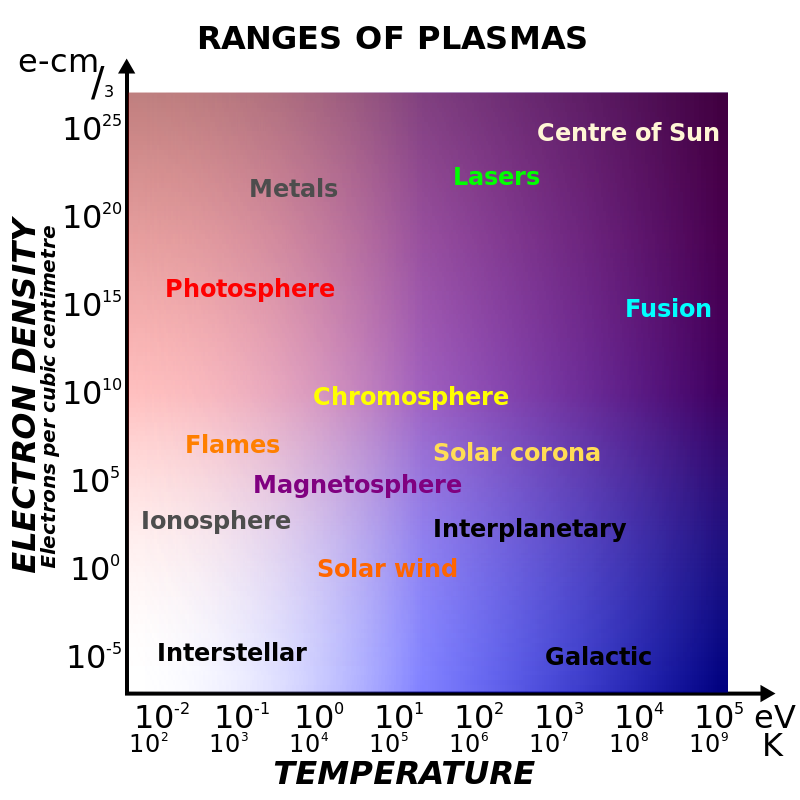
\includegraphics[scale=0.3]{faixaplasma.png}   
\caption{Aumento da densidade para cima, aumento da temperatura para a direita \cite{figplasma}.}
\label{fig: plasmafaixa}
\end{figure}

A magnetohidrodinâmica (MHD) é a área da física que estuda a interação mútua entre fluidos condutores e campos eletromagnéticos. 
Os fluidos em questão devem ser eletricamente condutivos e não magnéticos, ou seja, os limita a metais líquidos, eletrolitos fortes e o caso que estudaremos neste trabalho, o plasma. 
A interação mútua de um campo magnético $\bm{B}$ e um plasma de velocidade $\bm{u}$, surge como resultado das leis de Faraday e Ampère, devido a força de Lorentz.  
Dividindo este processo em três partes, temos basicamente que:
\begin{enumerate}
\item O movimento de um fluido condutor em um campo magnético provoca uma força eletromotriz induzida (de ordem $|\bm{u} \times \bm{B} | $) de acordo com a lei de indução de Faraday.  Em geral, correntes elétricas ocorrerão, sendo a densidade de corrente de ordem $\sigma (\bm{u} \times \bm{B})$, onde $\sigma$ é a condutividade elétrica. 
\item Estas correntes induzidas devem, de acordo com a lei de Ampère, dar origem a um campo magnético induzido que se soma ao campo magnético original, fazendo com que o fluido "arraste" \ as linhas do campo magnético junto com ele. 
\item O campo magnético combinado (imposto mais induzido) interage com a densidade de corrente induzida $\bm{J}$ para dar origem a uma densidade de força de Lorentz $\bm{J} \times \bm{B}$ que age no fluido condutor inibindo seu movimento no  campo magnético.  
\end{enumerate} 

Note que os dois últimos efeitos implicam em consequências semelhantes.  
Em ambos, o movimento do fluido no campo magnético tende a ser reduzido. 
Os fluidos podem \ "arrastar" \ linhas de campo magnético (efeito 2) e campos magnéticos podem puxar fluidos condutores (efeito 3). 
É esse "congelamento" \ parcial do meio e do campo magnético que é a marca registrada do modelo MHD ideal (a resistividade do plasma é nula).  

Para a descrição do plasma, são duas as abordagens mais comuns: o modelo de fluidos e o modelo cinético. 
Cada um com suas vantagens e desvantagens. %A magnetohidrodinâmica (MHD) é um caso particular do modelo de 1 fluido que descreve o plasma por meio de quantidades macroscópicas simplificadas, como por exemplo a  densidade numérica de partículas e a densidade de corrente.que são um caso particular das equações de um fluido quando as partículas não possuem carga elétrica 
O modelo de um fluido trata o plasma como um fluido único que é governado pelas equações do eletromagnetismo de Maxwell e as equações de Navier-Stokes, com a adição da força de Lorentz. 
%Portanto não levam em conta forças de origem eletromagnética. 

Neste trabalho, será usada uma descrição mais geral do plasma, ou seja, um modelo de dois fluidos. Neste modelo os íons e os elétrons são descritos como dois fluidos diferentes. %Com uma distribuição de velocidades para elétrons e outra para íons. 
Os modelos de fluidos são precisos quando a distribuição de velocidade das espécies se aproxima da distribuição de Maxwell-Boltzmann, o que normalmente ocorre quando o grau de colisões é alto, ou seja, um plasma quente onde o grau de ionização é alto. 
%Uma desvantagem do modelo de fluidos é que devido a descrição do plasma em termos de um único fluxo a uma determinada temperatura em cada localização espacial. 
%O modelo não permite capturar flutuações no plasma, como raios de luz ou camadas duplas, nem descrever efeitos ondulatórios de partículas. 
O modelo cinético não precisa assumir uma distribuição de Maxwell-Boltzmann, já que adota uma função de distribuição de velocidades em cada ponto do plasma. Porém, o modelo cinético demanda muito mais computação para ser resolvido satisfatoriamente. Devido a esse excessivo aumento de demanda computacional e de uma maior complexidade, escolhe-se normalmente para a modelagem do \textit{breakdown} o modelo de fluidos.


\section{Fusão} 
\noindent A fusão nuclear é um processo físico promissor para suprir a crescente demanda energética. 
O sol é alimentado por reações de fusão assim como todas as estrelas. 
Em tais reações, núcleos de baixa massa se combinam, ou se fundem, para formar núcleos mais massivos. 
No sol, uma sequência de reações de fusão, denominada cadeia p-p, começa com prótons - núcleos de hidrogênio comum - termina com partículas alfa - núcleos de átomos de hélio. Após uma reação de fusão, as massas finais são menores do que as iniciais e a diferença de massa é convertida em energia, através da conhecida equação de Einstein,
$$ E = \Delta m c^2 ,$$ 
onde $E$ é a energia resultante da reação, $\Delta m$ é a diferença de massa e $c$ é a velocidade da luz no vácuo. 
A fissão nuclear apresenta vários problemas, como riscos de explosões, produção significativa de resíduos radioativos e usos militares. 
O processo de fusão, no entanto, é naturalmente seguro, embora a reação de fusão também produza resíduos radioativos. No entanto, tais subprodutos são as partículas $\alpha$ (núcleos de Hélio). 
O fluxo de nêutrons em um reator tornará os materiais estruturais radioativos. 
O trítio tem uma meia-vida de apenas 12 anos, enquanto a escolha apropriada de materiais pode resultar em resíduos que têm meias-vidas de dezenas de anos, em vez de milhares de anos, como na fissão. 
Outra enorme vantagem da fusão é que os materiais usados para reação de fusão podem ser extraídas da água do mar. 
Portanto, a fusão é considerada uma fonte de energia virtualmente inesgotável. 
Como a fusão deve ser continuamente alimentada, e sua manutenção depende estritamente do equilíbrio MHD, ela é facilmente interrompida. 
Mesmo nos piores acidentes imagináveis, o plasma contido no tokamak não terá energia suficiente para causar a ruptura da câmera de vácuo.

\section{Tokamak} 
\noindent O tokamak é um conceito de máquina de confinamento de plasmas que tem como objetivo criar condições onde a fusão nuclear aconteça. 
A palavra tokamak é a transliteração de um acrônimo russo que significa "câmara toroidal com bobinas magnéticas". 
O objetivo final da pesquisa com tokamaks é tornar viável a construção de reatores nucleares de fusão com balanço positivo de energia, ou seja, a energia extraída é maior que a gasta para manter as reações de fusão. 
A reação de fusão mais promissora é a de deutério e trítio. 
A grande quantidade de energia liberada servirá para aquecer água, produzir vapor e assim mover uma turbina acoplada a um gerador elétrico. 
%A pesquisa em tokamaks, portanto, está ligada à procura de fontes alternativas de energia para a produção de eletricidade. 

Basicamente, um tokamak é um potente eletroímã que produz um campo magnético toroidal. 
Um toróide é a configuração mais simples com linhas de campo magnético fechadas, condição está necessária para evitar a perda do plasma. %no entanto, um campo puramente toroidal varia com $\frac{1}{R}$. 
O gradiente da amplitude do campo magnético e a curvatura das linhas de campo levam a movimentos de íons e elétrons em direções verticais opostas, o que resulta em uma separação de cargas. Esta, por sua vez, cria um campo elétrico que, junto com o campo magnético produzirá uma deriva das partículas na direção radial. %uma corrente elétrica. A geometria toroidal da corrente causa em lados opostos, correntes opostas causando uma força que tende a empurrar para fora todo o plasma. 
Este movimento de deriva para fora pode ser evitado torcendo as linhas do campo magnético, de modo que cada linha de campo passe pelas partes superior e inferior do toroide. 
De tal forma que a média ao longo do caminho das partículas leve a um cancelamento dos movimentos de desvio verticais e evite o estabelecimento de um campo elétrico. 
Portanto, uma combinação de campos magnéticos toroidais e poloidais pode adequadamente confinar um plasma.
No interior da câmera de vácuo de um tokamak ocorre uma emissão de elétrons que são altamente acelerados pelo campo elétrico, que então provocam uma ruptura (\textit{breakdown}) do gás de trabalho gerando a corrente de plasma, que irá formar o plasma que deve ser contido no espaço limitado da câmera de vácuo. 
O campo magnético não pode permitir que o plasma toque nas paredes internas da câmera de vácuo, tanto para não danificá-la, quanto para não dissipar a energia do plasma via condução térmica ou contaminar o plasma com átomos e moléculas pesadas. 
O tokamak é ainda caracterizado pela simetria azimutal. 
Alguns tokamaks tem sessão reta da câmera retangular, como o TCABR da USP, enquanto outros possuem sessão reta circular, como o NOVA-FURG, ou até alongada em formato elíptico, como o ITER. 
Outra característica dos tokamaks é o uso da corrente de plasma para gerar a componente helicoidal do seu intenso campo magnético, necessária para um equilíbrio MHD \cite[pg. 34]{tokamaks}, \cite[pg. 10]{MagneticControl}. 
A Figura \ref{fig: Rotulotokamak01} mostra os componentes básicos de um tokamak, onde os termos "Campo poloidal"\ e "Campo toroidal"\ se referem aos campos eletromagnéticos. 
No tokamak NOVA-FURG as duas bobinas de aquecimento ôhmico (em azul na Figura \ref{fig: Rotulotokamak001}) fazem o papel de enrolamento primário do transformador da Figura \ref{fig: Rotulotokamak01}, e a corrente de plasma faz o papel de enrolamento secundário do transformador.
Ao longo deste trabalho foi modelado no programa Blender o tokamak NOVA-FURG, respeitando as medidas de cada componente. O modelo pode ser visto na Figura \ref{fig: Rotulotokamak001} e uma imagem real da máquina na Figura \ref{fig: Rotulotokamak003}. 
O tokamak NOVA-FURG utiliza um núcleo de ferro como transformador ôhmico, possui uma parede de aço inox com uma camada condutora de alumínio e tratamento superficial da parede interna com titânio. E possui um filamento de tungstênio que fornece elétrons para ajudar no \textit{breakdown}.  
Detalhes dos parâmetros geométricos das bobinas do tokamak NOVA-FURG podem ser vistos na Tabela \ref{tab-nova} e na Figura \ref{fig: btokamak}. 
\begin{figure}[H]
\centering
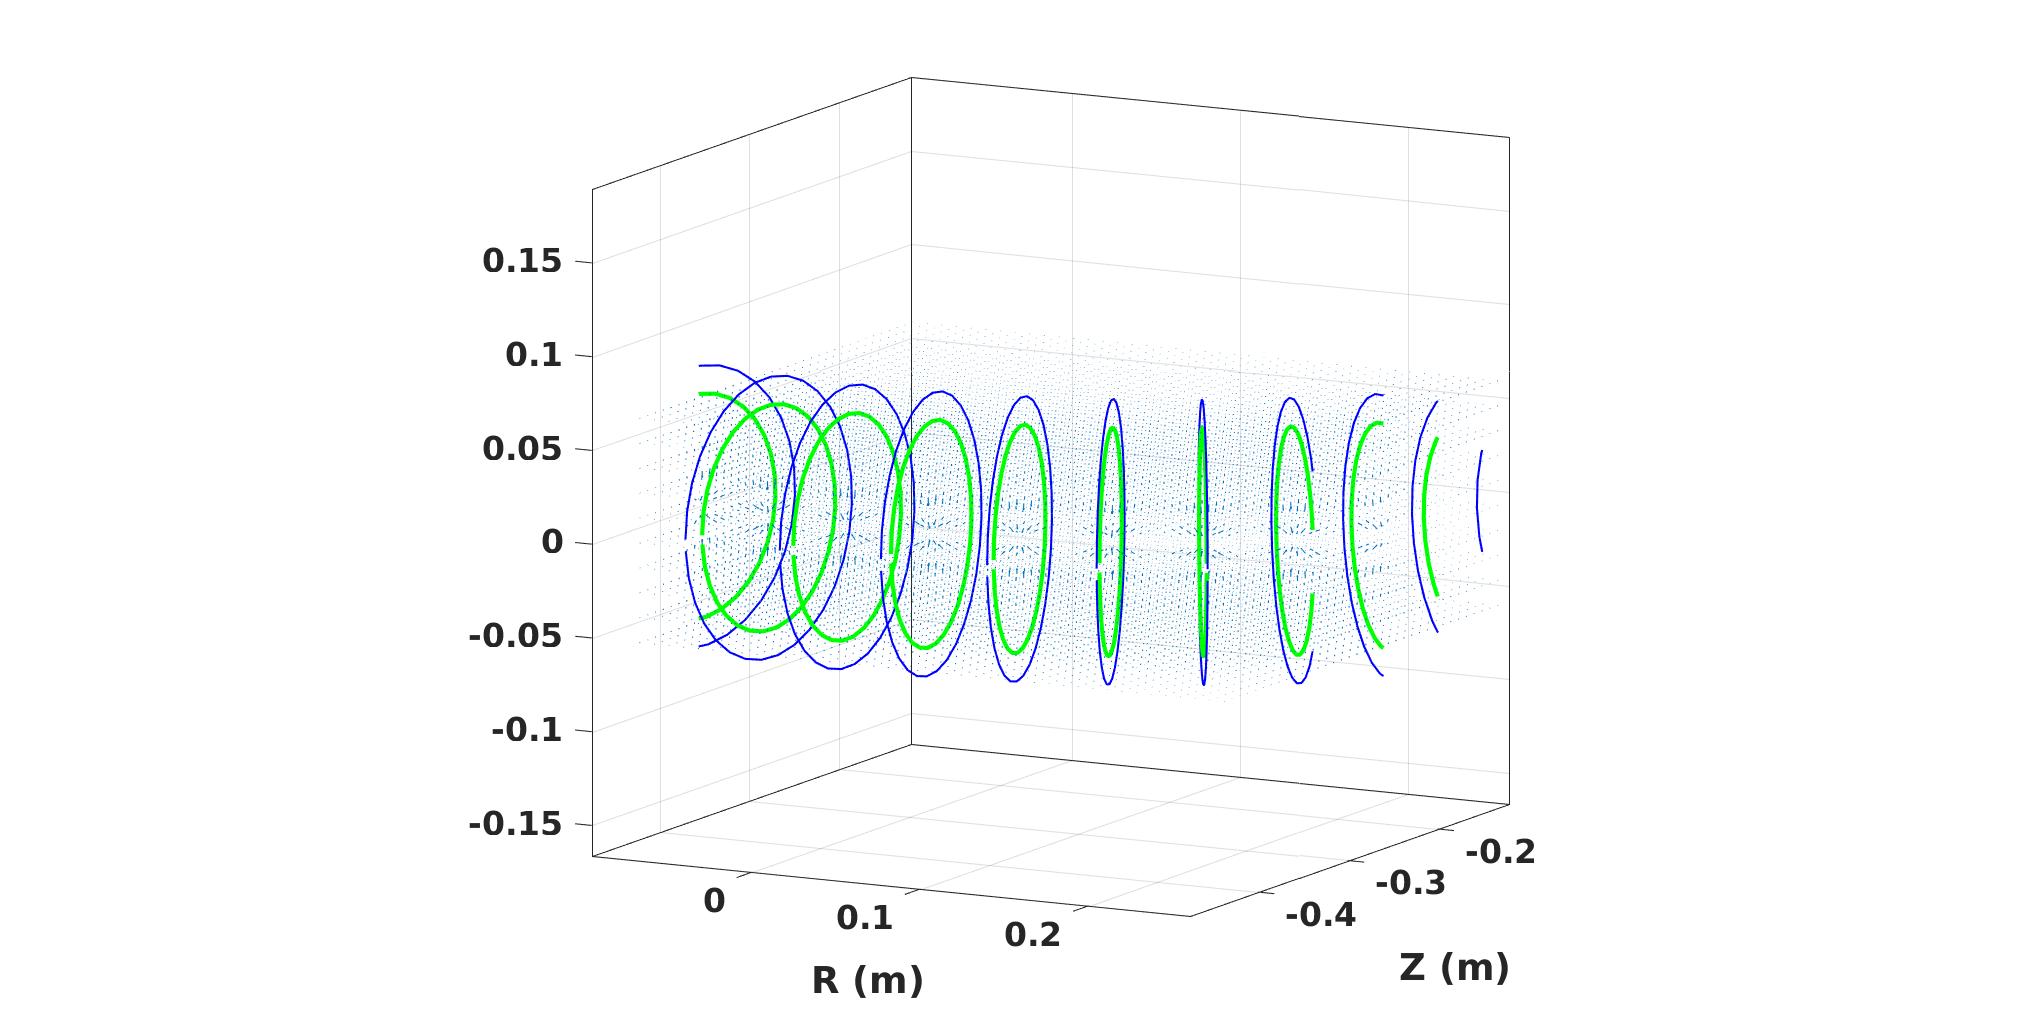
\includegraphics[scale=0.9]{../Rascunho_Resumo/tokamak.png} 
\caption{Esquema básico de um tokamak [Daltrini (1999), Ferrari e Nascimento (1988)].}
\label{fig: Rotulotokamak01}  
\end{figure}
\begin{figure}[H]
\centering
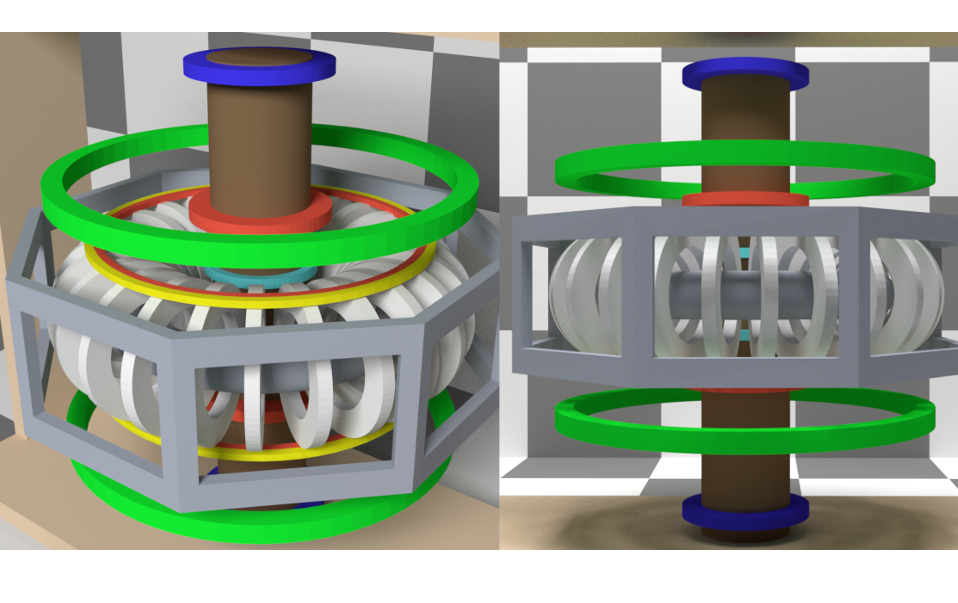
\includegraphics[scale=0.45]{tokamak12.png}
\caption{Tokamak NOVA-FURG, modelo feito no Blender.}    
\label{fig: Rotulotokamak001}
\end{figure}
\begin{figure}[H]
\centering
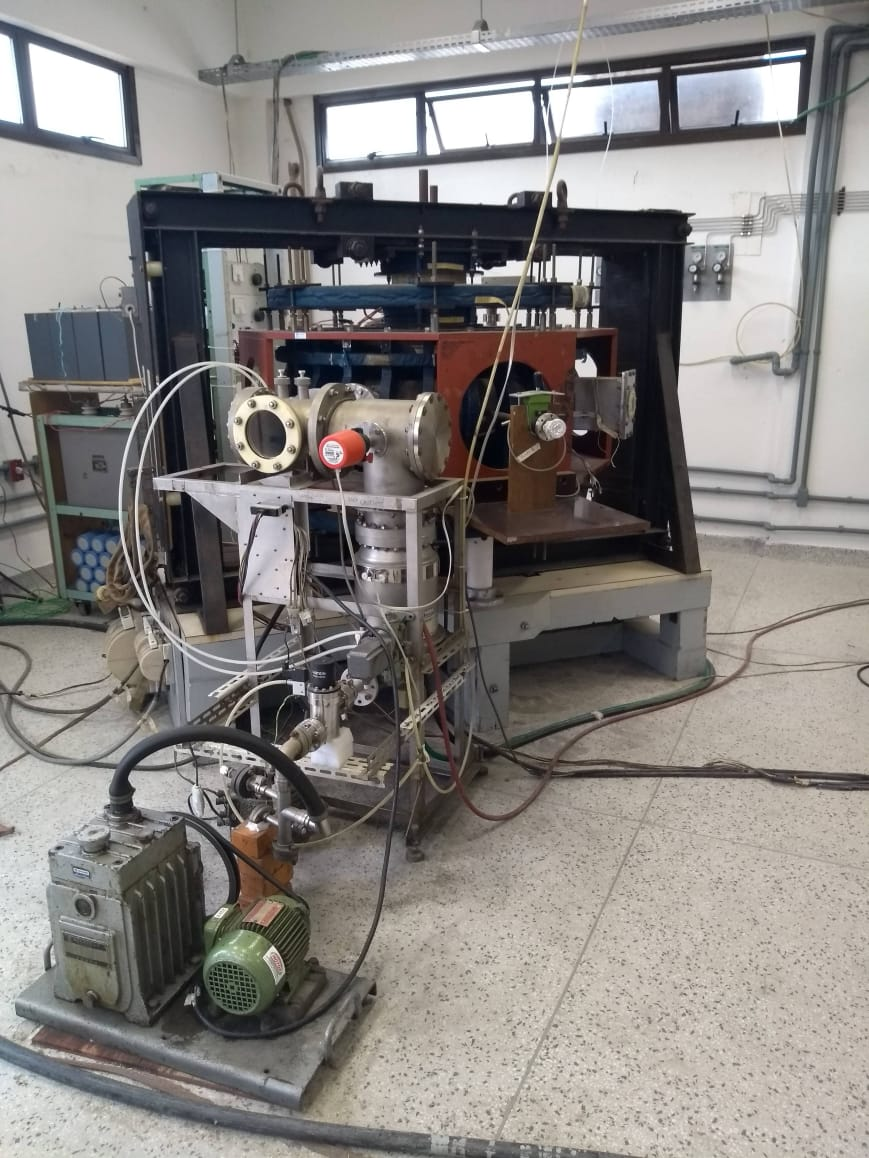
\includegraphics[scale=0.3]{../MPU19/tokamak.jpeg} 
\caption{Tokamak NOVA-FURG.}    
\label{fig: Rotulotokamak003}
\end{figure}
\section{Plasma \textit{startup}}
O início da operação de um tokamak consiste em três fases:
\begin{enumerate}
\item Fase de \textit{breakdown} do plasma (fase dominada pela avalanche de elétrons)
\item Fase de \textit{burn-through} (fase de ionização e aquecimento do plasma) 
\item Fase de \textit{current ramp-up} (estabelecimento da corrente de plasma).
\end{enumerate}
Na sequência, será dada uma breve descrição destas três fases, lembrando que o foco deste trabalho é a primeira fase. 

\subsection{Breakdown}
\noindent A fase de \textit{breakdown} em um tokamak é dominada por colisões entre elétrons livres e partículas neutras. A fase de \textit{breakdown} começa com a primeira ionização e dura até que as colisões de Coulomb comecem a dominar as colisões neutras com elétrons \cite[pg. 55]{sinha2017plasma}. %aqui foi pegado de referencia da pg 55 da tese brackdown e current formation
Este processo pode ser descrito pelo modelo desenvolvido por Townsend \cite{lloyd1991}. 
A descarga de Townsend (\textit{Townsend discharge}) é um processo de ionização de gás onde os elétrons livres, sob efeito de um campo elétrico intenso, são acelerados para então colidirem com moléculas de gás e liberarem elétrons adicionais, Figura \ref{avalanche}. 
Elétrons que também são acelerados, colidem e liberam mais elétrons adicionais, resultando em uma avalanche que permitirá a passagem de corrente pelo gás. Em um tokamak, o plasma parcialmente ionizado é condutor e uma corrente de plasma toroidal é formada devido ao campo elétrico toroidal.  
A descarga requer uma fonte de elétrons livres e um campo elétrico suficientemente intenso. 
O primeiro coeficiente de Townsend, explicado e modelado no apêndice \ref{Townsend}, corresponde ao número de reações de ionização, por unidade de comprimento, causadas por um elétron que se move paralelamente ao campo elétrico. 
O campo magnético poloidal, gerado pela corrente de plasma toroidal, começa a aumentar até que a corrente se estabiliza. 
São formadas então, superfícies de fluxo magnético fechadas que reduzem a perda de íons e elétrons, o que causa um aumento na taxa de crescimento da corrente de plasma. Uma explicação mais detalhada para a fase de \textit{breakdown} pode ser encontrada em \cite[pg. 40]{piras2011extremely}.

	\begin{figure}[H]
				\centering
			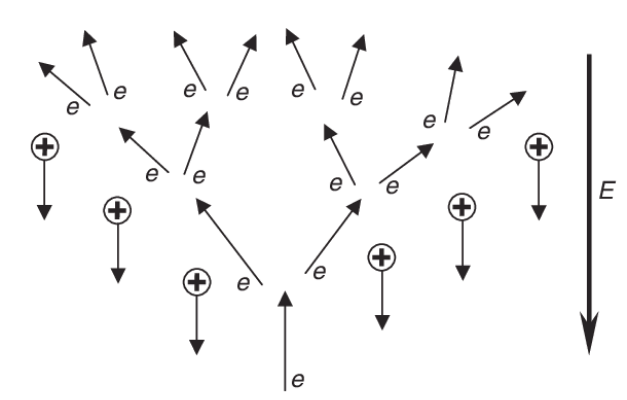
\includegraphics[scale=0.6]{avalanche.png} 
				\caption{Ilustração do breakdown de Townsend \cite{article0}.}
		\label{avalanche}
			\end{figure}
\subsection{Burn-through}
\label{burn-through}
%codigo usado para simular está fase: DYON (DYnamic0D model of Non-fully ionized plasma) code
\noindent A fase de \textit{burn-through} é caracterizada pelo aumento da corrente de plasma causada pelo aumento da ionização do plasma.
A ionização do gás neutro e radiações de linha das impurezas presentes no plasma, resultam na perda de uma parte significativa do poder de aquecimento \cite{breacdown, breacdown2}. Esta perda de potência é proporcional ao produto da densidade de elétrons com a densidade de partículas neutras, e tem seu máximo na chamada barreira de radiação. O plasma precisa "queimar" \ essa barreira de radiação antes que a potência de aquecimento possa elevar a temperatura do plasma. 
Um estado de alta ionização de impurezas é normalmente alcançado após a "queima" \ do gás principal. 
Uma "queima" \ (\textit{burn-through}) de plasma bem sucedida só pode ser obtida se a potência de aquecimento ôhmico exceder a perda de potência por ionização e radiação. 
Depois que a queima é realizada, a corrente de plasma é tipicamente aumentada até que o valor máximo de corrente de plasma (\textit{flattop}) seja atingido. 
Durante a fase de aceleração da corrente de plasma (\textit{ramp up} \ref{ramp-up}), é essencial evitar interrupções causadas por instabilidades MHD. 
As fases de \textit{breakdown}, \textit{burn-through} e \textit{ramp-up} não são necessariamente fases consecutivas, mas processos que podem ocorrer simultaneamente. 
É fundamental para o funcionamento do tokamak a obtenção da configuração de superfícies de fluxo fechado. Para isso, a corrente de plasma deve crescer e o gás combustível deve ser totalmente ionizado durante a fase de queima de plasma (\textit{burn-through}).
Uma das características cruciais na fase de \textit{burn-through} é a transição da configuração do campo magnético, ou seja, a mudança de configuração de linhas de campo abertas para as superfícies de fluxo fechadas. A Figura \ref{fig: burn-through} mostra dados típicos da fase de \textit{burn-through} no tokamak JET. Mais detalhes da fase de \textit{burn-through} podem ser encontrados em \cite{breacdown, kim2013plasma}.

\begin{figure}[h]
\centering
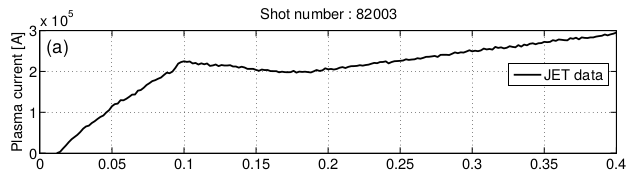
\includegraphics[scale=0.4]{burn-through-phase.png} 
\caption{Dados experimentais típicos de corrente de plasma medidos durante a fase de \textit{burn-through} no tokamak
JET \cite{kim2013physics}.}   
\label{fig: burn-through}
\end{figure}
%O código comumente usado na literatura para realizar simulações da fase de \textit{burn-through} é o DYON (DYnamic0D model of Non-fully ionized plasma).
\subsection{Ramp-up}
\label{ramp-up}
\noindent A fase de \textit{ramp-up} inicia-se após a queima do gás principal, mas é independente da quantidade de impurezas, podendo, então, se sobrepor à fase de \textit{burn-through}. A Figura \ref{fig: tokamakphases} apresenta um diagrama de como são caracterizadas, ao longo do tempo, as fases de \textit{breakdown}, \textit{burn-through} e \textit{ramp-up}.  Uma explicação mais detalhada para a fase de \textit{ramp-up} pode ser encontrada em \cite[pg. 49]{piras2011extremely}. A Figura \ref{fig: tokamakphases} apresenta um diagrama com as três fases ilustradas.

\begin{figure}[H]
\centering
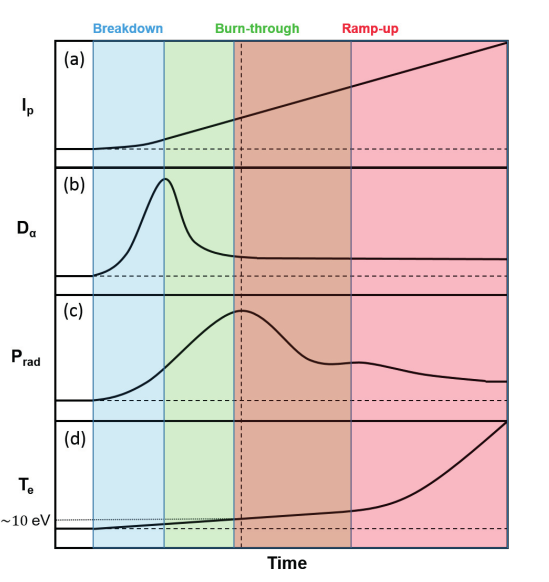
\includegraphics[scale=0.4]{tabela3fases.png}  
\caption{Figura esquemática da evolução temporal da (a) corrente de plasma, (b) emissão de $D_\alpha$, (c) perda de potência de radiação e ionização e (d) temperatura do elétron em uma formação típica de plasma de deutério. As fases de \textit{breakdown} (azul), \textit{burn-through} (verde), de \textit{ramp-up} (vermelho) e a sobreposição entre a fase de \textit{burn-through} e a fase de \textit{ramp-up} (marrom) são marcadas com as respectivas cores. A linha tracejada vertical representa a barreira de radiação \cite{sinha2017plasma}.}    
\label{fig: tokamakphases}
\end{figure}


\section{Função de distribuição}
\noindent A função de distribuição $f$ é uma função que contém informação sobre a densidade de partículas com posição entre $\bm{r}$ e $\bm{r}+d\bm{r}$ e velocidade entre $\bm{v}$ e $\bm{v}+d\bm{v}$. Definida num espaço de fase de seis dimensões, sendo três de posição e três de velocidade, a distribuição Maxwelliana \cite[pg. 127]{bittencourt} é dada por:
\begin{equation}
\label{distmax}
    f(\bm{r}, \bm{v}) = n(\bm{r}) \Big(\frac{m}{2\pi k_B T(\bm{r})}\Big)^{\frac{3}{2}}\exp\Big(\frac{-mv^2}{k_B T(\bm{r})}\Big),
\end{equation}
onde $n(\bm{r})$ é a densidade de partículas no espaço de configuração, $T(\bm{r})$ é a temperatura do plasma, $m$ é a massa das partículas, $\bm{v}$ é a velocidade e $k_B$ é a constante de Boltzmann. Quando o plasma está em equilíbrio termodinâmico a função de distribuição se torna Maxwelliana, conforme o teorema de Boltzmann.
Na maioria dos plasmas de laboratório, o estudo é feito fora do equilíbrio termodinâmico, uma vez que sempre se tem a variação de alguma propriedade macroscópica no plasma. Frequentemente estudos são feitos considerando que o plasma está em um certo equilíbrio, por exemplo elétrons estão em equilíbrio entre si a uma temperatura $T_e(\bm{r})$ e íons em equilíbrio entre si a uma temperatura $T_i(\bm{r})$. Investiga-se o que acontece com a distribuição a partir deste estado que se chama meta-equilíbrio.
A partir de $f$, obtemos a velocidade média
\begin{equation}
    <v> = \sqrt{\frac{8k_BT}{m\pi}},
    \end{equation} 
 a velocidade mais provável 
\begin{equation}
   v_{max}=\sqrt{\frac{2k_BT}{m}}
   \end{equation}   
e a velocidade quadrática média
\begin{equation}
   v_{rms}=\sqrt{\frac{3k_BT}{m}}.
   \end{equation} 
\section{Momentos da distribuição de Maxwell}
\noindent A função de distribuição é uma descrição microscópica de um plasma. Em contraste, uma descrição macroscópica de um plasma se faz pela especificação de valores médios das propriedades do plasma, tais como a densidade, velocidade média e pressão. A densidade de partículas da espécie $\alpha$ é dada por
\begin{equation*}
    n_\alpha(\bm{r},t) = \int_V f_\alpha(\bm{r},\bm{v},t) d^3 v,
\end{equation*}
a velocidade média das partículas da espécie $\alpha$ é
\begin{equation*}
    \bm{u}_\alpha(\bm{r},t) = \frac{1}{n_\alpha(\bm{r},t)} \int_V \bm{v} f_\alpha(\bm{r},\bm{v},t) d^3 v
\end{equation*}
e o tensor de pressão das partículas da espécie $\alpha$,
\begin{equation*}
    \mathbb{P}_\alpha(\bm{r},t) = \frac{m_\alpha}{n_\alpha(\bm{r},t)}\int_V (\bm{v}-\bm{u}_\alpha)(\bm{v}-\bm{u}_\alpha) f_\alpha(\bm{r},\bm{v},t) d^3 v,
\end{equation*}
onde $V$ é o espaço de velocidades.
%\int f_\alpha(\bm{r},\bm{v},t) \frac{d\bm{v}}{n_\alpha\bm{r}}

\chapter{Objetivos}
\noindent Na fase teórica deste trabalho pretende-se desenvolver um modelo de dois fluidos para o \textit{breakdown} em plasmas do tokamak NOVA-FURG. Para isso, primeiro temos de obter a equação geral dos momentos da equação de Boltzmann.
Após a dedução das equações para os três primeiros momentos da equação de Boltzmann, para elétrons e íons, o sistema será simplificado de acordo com as condições pertinentes a fase de \textit{breakdown} em tokamaks de pequeno porte. 
A fase computacional tem o propósito de resolver o sistema obtido na fase teórica, a fim de obter os parâmetros macroscópicos do plasma ao longo da fase de \textit{breakdown}, onde a corrente de plasma ainda é pequena permitindo que se admita que os campos elétrico e magnético gerados pelo plasma sejam nulos. 
Tendo então as distribuições ao longo dos tempos iniciais para os parâmetros do plasma, será verificado se os resultados condizem com o comportamento esperado do plasma.
Pretende-se após a realização das simulações numéricas interpretar fisicamente os resultados para cada variável macroscópica do modelo de 2 fluidos.  

\chapter{Revisão Bibliográfica}
\noindent Por volta de 1950 já existia alguns trabalhos sobre o modelo cinético e de fluidos. 
Nesta mesma época os físicos soviéticos Igor Tsamm e Andrei Sakharov sugeriram unir as pontas das máquinas líneares em um formato de toróide, visando melhorar o confinamento. 
Essa configuração foi chamada de tokamak. 
Ainda na mesma década, em 1958, Kruskal e  Kulsrud \cite{Kruskal1958} apresentaram algumas propriedades gerais do plasma usando as equações MHD, ou seja, equação da conservação da massa, do momento e da energia, juntamente com as equações de Maxwell e lei de Ohm. 
Ao longo de quase duas décadas, a pesquisa com o modelo de fluidos de plasmas confinados em tokamaks avançou muito. 
Em 1979 Hirshman e Jardin \cite{hirshman} publicam um artigo onde deduzem equações de transporte de dois fluidos. 
Dois anos depois é publicado por Sakanaka (1981) \cite{Sakanaka1981} uma dedução detalhada das equações de transporte a partir dos momentos da equação de Boltzmann. 

Com a construção de grandes tokamaks ao redor do mundo, os modelos de fluidos vieram a ser amplamente desenvolvidos para modelar o plasma nestes novos tokamaks. 
Foi usado por Zakharov e Rogers (1989-1993) \cite{Zakharov} um modelo linearizado de dois fluidos para a descrição do modo de \textit{kink} interno em tokamaks. 
Uma abordagem computacional baseada na evolução das equações de movimento de plasma eletromagnético, não linear e de dois fluidos foi usada por Thyagaraja (2000) \cite{Thyagaraja_2000} para investigar as propriedades da turbulência e do transporte do plasma tokamak. 
Pode-se ver mais detalhes sobre o \textit{breakdown} nos artigos de B. Lloyd, P. G. Carolan e C. D. Warrick (1996) \cite{breacdown} e D Mueller (2013) \cite{breacdown2}. 
Um estudo aprofundado juntamente com a realização de simulações numéricas das fases iniciais de operação de um tokamak é feito por Kim, Hyun Tae  \cite{kim2013physics} (2013). E por Sinha e Joyeeta \cite{sinha2017plasma} (2017) é feito um estudo aprofundado das três etapas iniciais do tokamak com muitos dados experimentais e comparações.  Em 1976 Hinton e Hazeltine \cite{RevModPhys.48.239} aprofundam o estudo sobre a teoria do transporte de plasma em sistemas de confinamento toroidal. Em 1989 Harafuji, Kenji, Hayashi, Takaya e Tetsuy \cite{harafuji1989computational} fizeram um estudo computacional dos equilíbrios MHD tridimensionais em sistemas helicoidais toroidais. Em \cite{weisstein2003toroidal}, o leitor pode conferir expressões em termos do seno e cosseno hiperbólico para os operadores diferenciais e em \cite{grimm1983ideal} pode-se conferir cálculos de estabilidade de MHD ideal em sistemas de coordenadas toroidais axissimétricos. Baseado nestes trabalhos será deduzido no apêndice \ref{pseudo-toroidaiss} o sistema de coordenadas pseudo-toroidais.

Como visto anteriormente, o uso dos modelos de fluidos é preferível em plasmas muito quentes e tem a vantagem de ser mais leve computacionalmente que os modelos cinéticos, como neste trabalho não iremos investigar efeitos microscópicos, um modelo de fluidos é o mais indicado. 


\begin{comment}
\chapter{Cronograma}
O cronograma do trabalho encontra-se na Tabela \ref{tab-cronograma}, onde as etapas são:

\begin{enumerate}
\item Levantamento bibliográfico;
\item Fase teórica:
\subitem Elaboração de uma introdução 
\subitem Dedução do modelo de 2 fluidos;
\subitem Simplificações cabíveis do modelo de 2 fluidos para o\textit{breakdown} no tokamak NOVA-FURG; 
\item Fase computacional:
\subitem Decidir a abordagem que será usada, se será explícita no tempo ou explícita e qual o melhor método numérico a ser usado no sistema;
\subitem  Implementação do modelo de 2 fluidos no MATLAB;
\subitem Definir as condições de contorno e fronteira;
\subitem Fazer diferentes simulações;
\item Análise dos resultados:
\subitem Relatório;
\subitem Síntese dos resultados;
\end{enumerate}

\begin{table}[h!]\begin{center}

	\begin{tabular*}{\textwidth}{@{\extracolsep{\fill}} c c c c c c c c c c c c}
		\toprule
		& Etapa & mar. & abr. & maio & jun. & jul. & ago. & set. & out. & nov. &\\
		\midrule
		&   1   &   x  &   x  &      &      &   x  &      &      &  x   &      &\\
		&   2   &   x  &   x  &   x  &   x  &      &      &      &      &      &\\
		&   3   &      &      &      &      &   x  &   x  &   x  &   x  &   x  &\\
		&   4   &      &      &      &      &      &      &      &   x  &   x  &\\
		\bottomrule                             
	\end{tabular*}
	\caption{Cronograma}\label{tab-cronograma}
\end{center}\end{table}

   \end{comment}

\chapter{Fase Teórica}
\label{faseteorica}
\noindent A fase teórica se inicia com uma dedução do modelo de 2 fluidos. 
Partindo da equação de Boltzmann, uma equação geral dos momentos é obtida, permitindo a dedução da equação de conservação da massa, do momento e da energia. 
O sistema de equações diferenciais parciais simplificado será escrito em termos da densidade de corrente. 
 
\section{Equação de Boltzmann}
\noindent De acordo com o modelo de fluidos, para descrever a dinâmica de um plasma, consideramos que os movimentos das partículas do plasma são governados pelos campos externos aplicados mais os campos internos gerados pelo plasma. O problema de obter o campo eletromagnético gerado pelo plasma, no entanto, ainda é complexo e requer uma solução auto-consistente com as equações de Maxwell.
A equação de Boltzmann é uma equação diferencial parcial usada para descrever a evolução temporal da função de distribuição $f_\alpha(\bm{r},\bm{v},t)$ no espaço das velocidades, posições e tempo. Em outras palavras, $f_\alpha(\bm{r},\bm{v},t)$ descreve a evolução temporal do sistema no espaço de fase \cite[pg. 193]{bittencourt}.
\begin{equation}
\label{eq: boltsmam}
\frac{\partial f_\alpha(\bm{r},\bm{v},t)}{\partial t} +\bm{v} \cdot \bm{\nabla} f_\alpha(\bm{r},\bm{v},t) + \bm{a} \cdot \bm{\nabla}_v f_\alpha(\bm{r},\bm{v},t) = \left( \frac{\delta f_\alpha}{\delta t} \right)_{coll} ,
\end{equation}   %\bm{C}_\alpha
onde $\bm{v}$ é a velocidade, $ \left( \frac{\delta f_\alpha}{\delta t} \right)_{coll} = \sum_\beta  \left( \frac{\delta f_\alpha}{\delta t} \right)_{\alpha \beta}$\{$f_\alpha$, $f_\beta$\} é o operador de colisão e os operadores diferenciais $\bm{\nabla}_v$ e $\bm{\nabla}$ em coordenadas cartesianas são 
$$\bm{\nabla}_v f_\alpha(\bm{r},\bm{v},t) =  \frac{\partial f_\alpha(\bm{r},\bm{v},t)}{\partial v_x} \hat{e}_{v_x} + \frac{\partial f_\alpha(\bm{r},\bm{v},t)}{\partial v_y} \hat{e}_{v_y} + \frac{\partial f_\alpha(\bm{r},\bm{v},t)}{\partial v_z} \hat{e}_{v_z}, $$  
$$\bm{\nabla} f_\alpha(\bm{r},\bm{v},t) = \frac{\partial f_\alpha(\bm{r},\bm{v},t)}{\partial x} \hat{e}_{x} + \frac{\partial f_\alpha(\bm{r},\bm{v},t)}{\partial y} \hat{e}_{y} + \frac{\partial f_\alpha(\bm{r},\bm{v},t)}{\partial z} \hat{e}_{z}$$
substituindo na eq. \ref{eq: boltsmam} os campos suavizados produzidos pelo plasma, obtêm-se então
\begin{equation}
\label{eq: boltzzz}
\frac{\partial f_\alpha(\bm{r},\bm{v},t)}{\partial t} +\bm{v} \cdot \bm{\nabla} f_\alpha(\bm{r},\bm{v},t) + \frac{1}{m_\alpha}[\bm{F}_{ext}+\bm{E}_{pl}+\bm{v} \times \bm{B}_{pl}] \cdot \bm{\nabla}_v f_\alpha(\bm{r},\bm{v},t)= \left( \frac{\delta f_\alpha}{\delta t} \right)_{coll},
\end{equation}
onde $\bm{F}_{ext}$ representa a força externa, incluindo a força de Lorentz associada a quaisquer campos elétrico e magnético aplicados externamente, e $\bm{E}_{pl}$ e $\bm{B}_{pl}$ são campos elétrico e magnético causados pela presença e movimento de todas as partículas carregadas dentro do plasma. Os campos eletromagnéticos $\bm{E}_{pl}$ e $\bm{B}_{pl}$  devem satisfazer as equações de Maxwell, uma vez que precisam ser consistentes com as densidades de carga e corrente macroscópicas existentes no próprio plasma
\begin{equation}
\label{eq: max1}
\bm{\nabla} \cdot \bm{E}_{pl} = \frac{\rho}{\epsilon_o},
\end{equation}
\begin{equation}
\label{eq: max2}
\bm{\nabla} \cdot \bm{B}_{pl} = 0,
\end{equation}
\begin{equation}
\label{eq: max3}
\bm{\nabla} \times \bm{E}_{pl} = -\frac{\partial \bm{B}_{pl}}{\partial t},
\end{equation}
\begin{equation}
\label{eq: max4}
\bm{\nabla} \times \bm{B}_{pl} = \mu_0 (\bm{J} + \epsilon_0 \frac{\partial \bm{E}_{pl}}{\partial t} ).
\end{equation}
Aqui $\mu_0 = 4\pi \times 10^{-7}$ [$N$ / $A^2$] é a permeabilidade magnética do vácuo, $\epsilon_0 = \frac{1}{\mu_0 c^2}$ é a permissividade elétrica do vácuo, $c$ a velocidade da luz no vácuo. 
A densidade de carga do plasma $\rho$ é dada por
\begin{equation}
\label{eq: rho}
\rho(\bm{r},t) = \sum_\alpha q_\alpha n_\alpha = \sum_\alpha q_\alpha \int_V f_\alpha(\bm{r},\bm{v},t) d^3v,
\end{equation}
e a densidade de corrente de plasma $\bm{J}$ é dada por
\begin{equation}
\label{eq: densidadecorrente}
\bm{J}(\bm{r},t) = \sum_\alpha q_\alpha n_\alpha \bm{u}_\alpha(\bm{r},t) = \sum_\alpha  q_\alpha \int_V \bm{v} f_\alpha(\bm{r},\bm{v},t) d^3v.
\end{equation}
Aqui $ \bm{u}_\alpha(\bm{r},t)$ denota a velocidade macroscópica do fluido (apêndice \ref{anexo1}). As equações eq. \ref{eq: boltzzz}, eq. \ref{eq: max1}, eq. \ref{eq: max2}, eq. \ref{eq: max3}, eq. \ref{eq: max4}, eq. \ref{eq: rho} e eq. \ref{eq: densidadecorrente} constituem um conjunto completo de equações a serem resolvidas ao mesmo tempo. %Então, por exemplo, em um procedimento iterativo, assumindo valores aproximados iniciais para $\bm{E}_{pl}(\bm{r}, t)$ e $\bm{B}_{pl}(\bm{r}, t)$, a eq. \ref{eq: boltzzz} pode ser resolvida para produzir $f_\alpha(\bm{r},\bm{v},t)$ para os tipos diferentes de partículas. A utilização dos valores calculados na eq. \ref{eq: rho} e eq. \ref{eq: densidadecorrente} leva a valores para as densidades de carga e corrente no plasma, que podem ser substituídas nas equações de Maxwell e resolvidas para $\bm{E}_{pl}(\bm{r}, t)$ e $\bm{B}_{pl}(\bm{r}, t)$. Esses valores são então introduzidos novamente na equação de Boltzmann (eq. \ref{eq: boltzzz}), e assim por diante, para obter uma solução auto-consistente para a função de distribuição de partículas individuais. %Embora a equação eq. \ref{eq: boltzzz} não inclua explícitamente um termo de colisão no seu lado direito e portanto, não leve em consideração colisões de curto alcance, ela é mais geral do que parece, já que uma considerável parte dos efeitos de interações de partículas já foram incluídas na força de Lorentz, por meio dos campos eletromagnéticos suavizados auto-consistentes internos. 
Não é necessário resolver a equação de Boltzmann para encontrar as variáveis macroscópicas de interesse físico. Estas variáveis estão relacionadas com os momentos da equação de Boltzmann. %As equações de transporte podem ser obtidas tomando os momentos da equação de Boltzmann. 



\section{Momentos da distribuição}
\noindent Nesta sessão, será obtida da equação de Boltzmann, a equação geral dos momentos. 
Seja uma propriedade física $\chi(v)$ das partículas do plasma. Multiplicando cada termo da eq. \ref{eq: boltzzz} por $\chi(v)$ e integrando a equação resultante sobre todo o espaço de velocidade obtemos

\begin{equation}
\label{eq: pit3.01}
\int_V \chi \frac{\partial f_\alpha}{\partial t} d^3 v + \int_V \chi \bm{v} \cdot \bm{\nabla} f_\alpha d^3 v + \int_V \chi \bm{a} \cdot \bm{\nabla}_v f_\alpha d^3 v = \int_V \chi \left( \frac{\delta f_\alpha}{\delta t} \right)_{coll} d^3 v.
\end{equation}
Resolvendo cada integral separadamente,

\begin{equation}
\label{eq: pit4.01}
\int_V \chi \frac{\partial f_\alpha}{\partial t} d^3 v  = \frac{\partial }{\partial t} (\int_V \chi f_\alpha d^3 v)-\int_V \frac{\partial \chi}{\partial t} f_\alpha d^3 v.
\end{equation}
No entanto, desde que $\chi = \chi(\bm{v})$, sua derivada parcial em relação ao tempo é zero. Usando a definição de valores médios (anexo \ref{anexo1}), o rendimento fica
\begin{equation}
\label{eq: pit5.01}
\int_V \chi \frac{\partial f_\alpha}{\partial t} d^3 v = \frac{\partial}{\partial t} [n_\alpha<\chi>_\alpha],
\end{equation}

\begin{equation}
\label{eq: pit6.01}
\int_V \chi \cdot \bm{v} \bm{\nabla} f_\alpha d^3 v = \bm{\nabla} \cdot \left( \int_V \chi \bm{v} f_\alpha d^3 v \right) - \int_V \bm{\nabla} \chi \cdot \bm{v} f_\alpha d^3 v - \int_V \chi  f_\alpha \bm{\nabla} \cdot \bm{v}  d^3 v.
\end{equation}
Como visto anteriormente, $\chi = \chi(\bm{v})$, então seu gradiente é zero e as variáveis $\bm{r}$, $\bm{v}$ e $t$ são independentes, então o divergente de $\bm{v}$ também é zero, resultando em
\begin{equation}
\label{eq: pit7}
\int_V \chi \bm{v} \cdot \bm{\nabla} f_\alpha d^3 v = \bm{\nabla} \cdot [n_\alpha<\chi \bm{v}>_\alpha],
\end{equation}
\begin{equation}
\label{eq: pit8}
\int_V \chi \bm{a} \cdot \bm{\nabla}_v f_\alpha d^3 v = \int_V \bm{\nabla}_v \cdot (\bm{a} \chi f_\alpha)d^3 v - \int_V f_\alpha (\bm{a} \cdot \bm{\nabla}_v \chi) d^3 v - \int_V \chi  f_\alpha (\bm{\nabla}_v \cdot \bm{a})  d^3 v.
\end{equation}
A primeira integral desaparece porque a função de distribuição deve desaparecer para $\pm \infty$. A última integral na eq. \ref{eq: pit8} desaparece se assumirmos que
\begin{equation}
\label{eq: pit9}
\bm{\nabla}_v \cdot \bm{a} = \frac{1}{m_\alpha} \bm{\nabla}_v \cdot \bm{F} = 0,
\end{equation}
isto é, se o componente de força $F_j$ for independente do componente de velocidade correspondente $v_j$, uma vez que $\bm{\nabla}_v \cdot \bm{F} = \sum_j \frac{\partial F_j}{\partial v_j}$. Isto é verdade para a força devido a um campo magnético, $\bm{F} = q_\alpha \bm{v} \times \bm{B}$ porque $j$ também neste caso $F_j$ é independente de $v_i$.
\begin{equation}
\label{eq: pit10}
\int_V \chi \bm{a} \cdot \bm{\nabla}_v f_\alpha d^3 v = -n_\alpha<\bm{a} \cdot \bm{\nabla}_v \chi>_\alpha,
\end{equation}
\begin{equation}
\label{eq: pit11}
\int_V \chi \left( \frac{\delta f_\alpha}{\delta t} \right)_{coll} d^3 v = \left[\frac{\delta}{\delta t}(n_\alpha<\chi>_\alpha)\right].
\end{equation}
Combinando as eq. \ref{eq: pit5.01}, eq. \ref{eq: pit7}, eq. \ref{eq: pit10} e eq. \ref{eq: pit11} na eq. \ref{eq: pit3.01} obtemos finalmente 
\begin{equation}
\label{eq: pit12}
\frac{\partial }{\partial t}(n_\alpha<\chi>_\alpha) + \bm{\nabla} \cdot (n_\alpha<\chi \bm{v} >_\alpha) - n_\alpha<\bm{a} \cdot \bm{\nabla}_v \chi>_\alpha = 
\end{equation}
\begin{equation*}
=[\frac{\delta}{\delta t}(n_\alpha<\chi>_\alpha)].
\end{equation*}
Que é a equação geral dos momentos. Na sequência serão obtidas, através da equação geral dos momentos, as equações de conservação da massa, do momento e da energia.
\section{Equação de conservação da massa}
\noindent A equação de conservação da massa, também conhecida como equação da continuidade, garante que toda massa ganha ou perdida pelo sistema é quantificada no termo $S_\alpha$.
Essa equação pode ser obtida diretamente pela substituição, na eq. \ref{eq: pit12} do $\chi$ por $m_\alpha$. 
Definindo a densidade de massa como $ \rho_{m\alpha} = n_\alpha m_\alpha$ temos
\begin{equation}
\label{eq: pit13}
\frac{\partial \rho_{m\alpha}}{\partial t} + \bm{\nabla} \cdot (\rho_{m\alpha} \bm{u}_\alpha)  = S_\alpha, 
\end{equation}
onde o termo de colisão, $S_\alpha = \left[\frac{\delta \rho_{m\alpha}}{\delta t}\right]_{coll}$, representa a taxa na qual partículas do tipo $\alpha$ são produzidas ou perdidas, por unidade de volume, como resultado de colisões, de acordo com \cite[pg. 197]{bittencourt}.
Seja $\rho_\alpha(\bm{r},t)$ a densidade de carga dada por $\rho_\alpha(\bm{r},t)=n_\alpha q_\alpha$ e $\bm{J}_\alpha$ a densidade de corrente, dada por $\bm{J}_\alpha=\rho_\alpha \bm{u}_\alpha$, podemos reescrever a eq. \ref{eq: pit13} em termos da densidade de corrente se dividirmos a eq. \ref{eq: pit13} por $m_\alpha$ e  multiplicarmos por $q_\alpha$ obtendo a equação de conservação da carga elétrica
\begin{equation}
\label{eq: pit13.001}
\frac{\partial \rho_{\alpha}}{\partial t} + \bm{\nabla} \cdot \bm{J}_\alpha  = \frac{q_\alpha}{m_\alpha} S_\alpha.
\end{equation}
 

\section{Equação de conservação do momento}
\noindent A equação de conservação do momento afirma que a taxa de mudança do momento de um fluido $\alpha$ é devida às forças externas aplicadas no fluido, à força de pressão do próprio fluido e também pelas forças internas devido a colisões, dispersão e produção de partículas de plasma.
Para derivar a equação de conservação do momento, $\chi$ é substituído por $m_\alpha \bm{v}_\alpha$ na eq. \ref{eq: pit12}, ou seja,
\begin{equation}
\label{eq: p2}
\frac{\partial }{\partial t}(n_\alpha<m \bm{v}>_\alpha) + \bm{\nabla} \cdot (n_\alpha<m \bm{v}^2 >_\alpha) 
\end{equation}
\begin{equation*}
= n_\alpha<\bm{a} \cdot \bm{\nabla}_v m \bm{v}>_\alpha +[\frac{\delta}{\delta t}(n_\alpha<m \bm{v}>_\alpha)].
\end{equation*}
Definindo $\bm{v}_\alpha = \bm{c}_\alpha + \bm{u}_\alpha$, onde $\bm{c}_\alpha$ é a velocidade térmica das partículas e  $\bm{u}_\alpha$ é a velocidade do fluido. 
Vamos tratar de cada termo da eq. \ref{eq: p2} separadamente.
Aplicando a definição de valor médio (apêndice \ref{anexo1}) e como $ \rho_{m\alpha} = n_\alpha m_\alpha$, ficamos com $\frac{\partial }{\partial t} (n_\alpha <\chi>_\alpha)=\frac{\partial }{\partial t} (n_\alpha <m \bm{v}>_\alpha)$, mas $\bm{c}_\alpha$ não influencia no valor médio. Portanto, ficamos com $\frac{\partial }{\partial t} (\rho_{m\alpha} \bm{u}_\alpha)$. 
Aplicando a regra da cadeia na derivada parcial obtemos
\begin{equation}
\label{eq: pit14}
\frac{\partial }{\partial t} (\rho_{m\alpha} \bm{u}_\alpha) = \bm{u}_\alpha \frac{\partial \rho_{m\alpha}}{\partial t}+\rho_{m\alpha} \frac{\partial \bm{u}_\alpha}{\partial t}.
\end{equation} 
Substituindo $\chi$ pelo momento $m_\alpha \bm{v}_\alpha$ temos $\bm{\nabla} \cdot (n_\alpha <\chi \bm{v}>_\alpha) =  \bm{\nabla} \cdot (n_\alpha <m \bm{v} \bm{v}>_\alpha)$ e tirando $m_\alpha$ para fora da média, pois é constante, temos $\bm{\nabla} \cdot (n_\alpha m_\alpha < \bm{v} \cdot \bm{v}>_\alpha)$. %Nota-se que dentro do termo de média, $ \bm{v}_\alpha$ é igual $\bm{v}$, pois o tipo de partícula $\alpha$ já está representado na operação valor médio $< >_\alpha$, produzindo $\bm{\nabla} \cdot (\rho_{m\alpha} <\bm{v} \cdot \bm{v}>)$. 
Aplicando a definição de valor médio obtemos 
\begin{equation}
\label{eq: pit15}
\bm{\nabla} \cdot (\rho_{m\alpha} <\bm{v} \cdot \bm{v}>) = \bm{\nabla} \cdot ( \rho_{m\alpha}\bm{u}_\alpha \cdot \bm{u}_\alpha + \rho_{m\alpha}<\bm{c} \cdot \bm{c}>_\alpha)
\end{equation} 
já que $\bm{c} \cdot \bm{u} = 0$, uma vez que $\bm{c}$ é isotrópico e não contribui para o valor médio de $\bm{v}_\alpha$ que, por definição, é igual a $\bm{u}_\alpha$.  %vai em todas as direções
No termo seguinte, $n_\alpha<\bm{a} \cdot \bm{\nabla}_v m_\alpha \bm{v}>_\alpha$, rearranjamos os termos ficando com $n_\alpha<(m_\alpha \bm{a} \cdot \bm{\nabla}_v) \bm{v}>_\alpha$. Observando que massa vezes aceleração é força, $\bm{F} = \bm{a} \cdot m_\alpha $, temos $n_\alpha <(\bm{F} \cdot \bm{\nabla}_v)\bm{v}>_\alpha$, que nos da
\begin{equation}
\label{eq: pit16}
n_\alpha <(\bm{F} \cdot \bm{\nabla}_v)\bm{v}>_\alpha=n_\alpha<\bm{F}>_\alpha,
\end{equation}
pois $(\bm{F} \cdot \bm{\nabla}_v)\bm{v} = \bm{F} \cdot (\bm{\nabla}_v\bm{v})$ e $\bm{\nabla}_v\bm{v} = 1$. 
Definindo $\bm{R}_\alpha$ como sendo a soma da taxa de mudança de momento devido ao espalhamento com a taxa de mudança de momento devido à produção de partículas \cite[pg. 201]{bittencourt}, obtemos
\begin{equation}
\label{eq: pit17}
\bm{R}_\alpha = \left[\frac{\delta}{\delta t}(n_\alpha<m \bm{v}>_\alpha)\right]=\left[\frac{\delta}{\delta t}(\rho_{m\alpha}\bm{u}_\alpha)\right].
\end{equation}
Substituindo eq. \ref{eq: pit14}, eq. \ref{eq: pit15}, eq. \ref{eq: pit16}, eq. \ref{eq: pit17} em eq. \ref{eq: p2} obtemos
\begin{equation}
\label{eq: pit19}
\bm{u}_\alpha \frac{\partial \rho_{m\alpha}}{\partial t} + \rho_{m\alpha} \frac{\partial \bm{u}_\alpha}{\partial t}+ \bm{\nabla} \cdot (\rho_{m\alpha} \bm{u}_\alpha \bm{u}_\alpha)+
\end{equation} 
\begin{equation*}
+\bm{\nabla} \cdot (\rho_{m\alpha} <\bm{c} \cdot \bm{c}>_\alpha)-n_\alpha<\bm{F}>_\alpha=\bm{R}_\alpha.
\end{equation*}
Definindo o tensor $\mathbb{P}_\alpha=\rho_{m\alpha} <\bm{c} \cdot \bm{c}>_\alpha$, que representa a força por unidade de volume dentro do plasma devido aos movimentos aleatórios das partículas \cite[pg. 149]{bittencourt}, temos que
\begin{equation}
\label{eq: pit20}
\bm{\nabla} \cdot (\rho_{m\alpha} \bm{u}_\alpha \bm{u}_\alpha) =  \rho_{m\alpha}(\bm{u}_\alpha \cdot \bm{\nabla})\bm{u}_\alpha + [\bm{\nabla} \cdot (\rho_{m\alpha} \bm{u}_\alpha)]\bm{u}_\alpha.
\end{equation}
Fazendo a força igual a força de Lorentz temos 
\begin{equation}
\label{eq: pit20.1}
<\bm{F}>_\alpha = q_\alpha (\bm{E} + \bm{u}_\alpha \times \bm{B})
\end{equation} e substituindo as eq. \ref{eq: pit20} e eq. \ref{eq: pit20.1} em eq. \ref{eq: pit19}, teremos
\begin{equation}
\label{eq: pit21}
 \bm{u}_\alpha \frac{\partial \rho_{m\alpha}}{\partial t} + \rho_{m\alpha} \frac{\partial \bm{u}_\alpha}{\partial t}+ \rho_{m\alpha} (\bm{u}_\alpha \cdot \bm{\nabla})\bm{u}_\alpha+[\bm{\nabla} \cdot (\rho_{m\alpha} \bm{u}_\alpha)]\bm{u}_\alpha  =
\end{equation}
\begin{equation*}
n_\alpha q_\alpha (\bm{E} + \bm{u}_\alpha \times \bm{B})-\bm{\nabla} \cdot \mathbb{P}_\alpha + \bm{R}_\alpha.
\end{equation*}
Rearranjando estes termos, temos que
\begin{equation}
\label{eq: pit22}
\rho_{m\alpha} \left[\frac{\partial \bm{u}_\alpha}{\partial t} + (\bm{u} \cdot \bm{\nabla})\bm{u}_\alpha \right]+ \bm{u}_\alpha \left[ \frac{\partial \rho_{m\alpha}}{\partial t} + \bm{\nabla} \cdot (\rho_{m\alpha} \bm{u}_\alpha)  \right] = 
\end{equation}
\begin{equation*}
=\bm{R}_\alpha +n_\alpha q_\alpha (\bm{E} + \bm{u}_\alpha \times \bm{B})-\bm{\nabla} \cdot \mathbb{P}_\alpha.
\end{equation*}
No entanto, o segundo termo no lado esquerdo da eq. \ref{eq: pit22} é a equação de conservação de massa eq. \ref{eq: pit13}, %então se não considerarmos as colisões que levam à geração ou perda de partículas, ou seja $S_\alpha = 0$, podemos simplificar a equação para (se sp for zero \bm{R} também será pois ambos são devido à colisões) (isotropica: não à direção privilegiada, suas propriedades são as mesmas em qualquer direção)
\begin{equation}
\label{eq: pit23}
\rho_{m\alpha} \left[\frac{\partial \bm{u}_\alpha}{\partial t} + (\bm{u} \cdot \bm{\nabla})\bm{u}_\alpha \right] =  \bm{R}_\alpha+n_\alpha q_\alpha (\bm{E} + \bm{u}_\alpha \times \bm{B})-\bm{\nabla} \cdot \mathbb{P}_\alpha-\bm{u}_\alpha S_\alpha.
\end{equation}
O termo $-\bm{\nabla} \cdot \mathbb{P}_\alpha $ representa a força causada pelas variações aleatórias nas velocidades de cada partícula que é exercida em um volume unitário do plasma. 
Esta força em cada unidade de volume também inclui forças associadas à pressão escalar e forças de cisalhamento, que são as forças viscosas. No nosso caso, o efeito da viscosidade é pequeno de modo que os termos não-diagonais de $\mathbb{P}_\alpha$ podem ser desprezados. 
Além disso, no caso em que a distribuição de velocidades de cada tipo de partícula é isotrópica, os termos diagonais de $\mathbb{P}_\alpha$ são todos iguais e representam a pressão cinética escalar $p_\alpha$. 
Assim, desconsiderando o efeito de viscosidade e considerando uma distribuição de velocidade isotrópica, temos $\mathbb{P}_\alpha =  \mathbf{1} p_\alpha$, e a força por unidade de volume se torna $-\bm{\nabla} \cdot \mathbb{P}_\alpha = -\bm{\nabla} p_\alpha$ \cite[cap 6]{bittencourt}. Então a equação de conservação do momento para cada espécie de partícula fica
\begin{equation}
\label{eq: pit23.1}
\rho_{m\alpha} \left[\frac{\partial \bm{u}_\alpha}{\partial t} + (\bm{u} \cdot \bm{\nabla})\bm{u}_\alpha \right] =  \bm{R}_\alpha+n_\alpha q_\alpha (\bm{E} + \bm{u}_\alpha \times \bm{B}) -\bm{\nabla} p_\alpha - \bm{u}_\alpha S_\alpha.
\end{equation}
%para as duas espécies de partículas, elétrons $\alpha=e$ e íons $\alpha=i$
Reescrevendo em função da densidade de corrente, eq. \ref{eq: densidadecorrente}, lembrando que a densidade de carga é dada por $\rho_\alpha=n_\alpha q_\alpha$. 
A densidade de massa então é dada por $\rho_{m\alpha} = n_\alpha m_\alpha$, e a densidade de corrente é dada por $\bm{J}_\alpha=\rho_\alpha \bm{u}_\alpha$, podemos escrever a velocidade média de cada espécie de partículas em termos da densidade de corrente, através da seguinte relação
\begin{equation}
\bm{u}_\alpha=\frac{\bm{J}_\alpha}{\rho_\alpha}.
\end{equation}

Substituindo $\bm{u}_\alpha=\frac{\bm{J}_\alpha}{\rho_\alpha}$ na  eq. \ref{eq: pit23.1}, obtemos
\begin{equation}
\label{eq: pit23.2}
\rho_{m\alpha} \left[\frac{\partial \frac{\bm{J}_\alpha}{\rho_\alpha}}{\partial t} + (\frac{\bm{J}_\alpha}{\rho_\alpha} \cdot \bm{\nabla})\frac{\bm{J}_\alpha}{\rho_\alpha} \right] =  \bm{R}_\alpha+n_\alpha q_\alpha (\bm{E} + \frac{\bm{J}_\alpha}{\rho_\alpha} \times \bm{B}) -\bm{\nabla} p_\alpha
\end{equation}
que pode ser simplificado, ou seja,
\begin{equation}
\label{eq: pit23.3}
n_\alpha m_\alpha \left[\frac{1}{q_\alpha n^2_\alpha} \left( \frac{\partial \bm{J}_\alpha}{\partial t} n_\alpha-\frac{\partial n_\alpha}{\partial t} \bm{J}_\alpha\right) + (\frac{\bm{J}_\alpha}{n_\alpha m_\alpha} \cdot \bm{\nabla})\frac{\bm{J}_\alpha}{n_\alpha m_\alpha} \right] =  
\end{equation}
\begin{equation*}
\bm{R}_\alpha+n_\alpha q_\alpha (\bm{E} + \frac{\bm{J}_\alpha}{n_\alpha m_\alpha} \times \bm{B}) -\bm{\nabla} p_\alpha.
\end{equation*}
O termo $n_\alpha m_\alpha$ pode sair para fora do divergente por ser escalar. Então ficamos com
\begin{equation}
\label{eq: pit23.4}
\frac{m_\alpha}{q_\alpha} \frac{\partial \bm{J}_\alpha}{\partial t} -\frac{\bm{J}_\alpha m_\alpha}{q_\alpha n_\alpha} \frac{\partial n_\alpha}{\partial t}  + (\bm{J}_\alpha \cdot \bm{\nabla})\bm{J}_\alpha =  \bm{R}_\alpha+n_\alpha q_\alpha (\bm{E} + \frac{\bm{J}_\alpha}{n_\alpha m_\alpha} \times \bm{B}) -\bm{\nabla} p_\alpha.
\end{equation}
Aplicando a distributiva no termo da força de Lorentz,
\begin{equation}
\label{eq: pit23.5}
\frac{m_\alpha}{q_\alpha} \frac{\partial \bm{J}_\alpha}{\partial t} -\frac{\bm{J}_\alpha m_\alpha}{q_\alpha n_\alpha} \frac{\partial n_\alpha}{\partial t}  + (\bm{J}_\alpha \cdot \bm{\nabla})\bm{J}_\alpha = \bm{R}_\alpha+n_\alpha q_\alpha \bm{E} + \frac{q_\alpha}{m_\alpha} (\bm{J}_\alpha \times \bm{B}) -\bm{\nabla} p_\alpha.
\end{equation}
Da eq. \ref{eq: pit13.001}, temos que
\begin{equation}
\label{eq: pit23.6}
\frac{\partial n_\alpha}{\partial t} = \frac{1}{m_\alpha} S_\alpha -\frac{1}{q_\alpha} \bm{\nabla} \cdot \bm{J}_\alpha.
\end{equation}
Substituindo a eq. \ref{eq: pit23.6} na eq. \ref{eq: pit23.5} temos
\begin{equation}
\label{eq: pit23.7}
\frac{m_\alpha}{q_\alpha} \frac{\partial \bm{J}_\alpha}{\partial t} -\frac{\bm{J}_\alpha m_\alpha}{q_\alpha n_\alpha} \left( \frac{1}{m_\alpha} S_\alpha -\frac{1}{q_\alpha} \bm{\nabla} \cdot \bm{J}_\alpha  \right)  + (\bm{J}_\alpha \cdot \bm{\nabla})\bm{J}_\alpha =
\end{equation}
\begin{equation*}
 \bm{R}_\alpha+n_\alpha q_\alpha \bm{E} + \frac{q_\alpha}{m_\alpha} (\bm{J}_\alpha \times \bm{B}) -\bm{\nabla} p_\alpha.
\end{equation*}
Aplicando a distributiva,
\begin{equation}
\label{eq: pit23.800}
\frac{m_\alpha}{q_\alpha} \frac{\partial \bm{J}_\alpha}{\partial t} -\frac{\bm{J}_\alpha S_\alpha}{q_\alpha n_\alpha}+ \frac{\bm{J}_\alpha}{q^2_\alpha n_\alpha} \bm{\nabla} \cdot \bm{J}_\alpha   + (\bm{J}_\alpha \cdot \bm{\nabla})\bm{J}_\alpha =
\end{equation}
\begin{equation*}
 \bm{R}_\alpha+n_\alpha q_\alpha \bm{E} + \frac{q_\alpha}{m_\alpha} (\bm{J}_\alpha \times \bm{B}) -\bm{\nabla} p_\alpha.
\end{equation*}
Agrupando os termos multiplicados por $\bm{J}_\alpha$, obtemos finalmente,
\begin{equation}
\label{eq: pit23.80}
\frac{m_\alpha}{q_\alpha} \frac{\partial \bm{J}_\alpha}{\partial t} + \left[ \frac{1}{q^2_\alpha n_\alpha} ( \bm{\nabla} \cdot \bm{J}_\alpha ) -\frac{S_\alpha}{q_\alpha n_\alpha} + \bm{J}_\alpha \cdot \bm{\nabla} \right] \bm{J}_\alpha  +\bm{\nabla} p_\alpha=
\end{equation}
\begin{equation*}
 \bm{R}_\alpha+n_\alpha q_\alpha \bm{E} + \frac{q_\alpha}{m_\alpha} (\bm{J}_\alpha \times \bm{B}),
\end{equation*}
que é a equação de conservação de momento escrita em função da densidade de corrente, esta equação estabelece a condição necessária para garantir a conservação do momento do sistema.

\section{Equação de conservação da energia}
\noindent  Para derivar a equação de conservação da energia, substituímos na eq. \ref{eq: pit12} o $\chi (\bm{v}_\alpha)$ por $\frac{m_\alpha \bm{v}^2_\alpha}{2}$, obtendo
\begin{equation}
\label{eq: p3}
\frac{\partial }{\partial t}(n_\alpha<\frac{1}{2}m v^2>_\alpha) + \bm{\nabla} \cdot (n_\alpha<\frac{1}{2}m v^2 \bm{v} >_\alpha) +
\end{equation}
\begin{equation*}
- n_\alpha<\bm{a} \cdot \bm{\nabla}_v \frac{1}{2}m v^2>_\alpha = [\frac{\delta}{\delta t}(n_\alpha<\frac{1}{2}m v^2>_\alpha)] .
\end{equation*}
O primeiro termo da eq. \ref{eq: p3} será simplificado trocando $ n_\alpha m_\alpha$ por $\rho_{m\alpha}$, 
\begin{equation}
\label{eq: pit24}
\frac{\partial }{\partial t}(n_\alpha<\frac{m \bm{v}^2}{2}>_\alpha)=\frac{\partial }{\partial t}(\frac{\rho_{m\alpha}}{2}<\bm{v}^2>_\alpha)
\end{equation}
Após ser rearranjado, a eq. \ref{eq: pit24} fica
\begin{equation}
\label{eq: pit24.1}
\frac{\partial }{\partial t}(\frac{\rho_{m\alpha}}{2}<\bm{v}^2>_\alpha)=\frac{\partial }{\partial t}(\frac{\rho_{m\alpha}}{2}(\bm{u}_\alpha \cdot \bm{u}_\alpha) + \frac{\rho_{m\alpha}}{2}<\bm{c} \cdot \bm{c}>_\alpha) .
\end{equation} 
Como a velocidade aleatória $\bm{c}_\alpha$ é isotrópica, temos que para qualquer partícula, $|\bm{v}^2| = v_x^2 + v_y^2 + v_z^2$, e como são muitas partículas que se movem em direções aleatórias, os valores médios dos quadrados das componentes de suas velocidades são iguais, logo, $v_x^2 = \frac{1}{3} |\bm{v}^2|$. Então da teoria cinética dos gases, obtemos $p=\frac{nMv_x^2}{V}$ onde $M$ é a massa molar do gás de trabalho, $p$ é a pressão e $n$ o numero de moles. No nosso caso $\frac{nMv_x^2}{V} = \frac{nM <c^2_\alpha>}{3V} $ e a densidade de massa $ \rho_{m\alpha} = n_\alpha m_\alpha$ pode subtituir $\frac{nM}{V}$ nos deixando com $\rho_{m\alpha}<c^2_\alpha>=3p_\alpha$ \cite[pg. 152]{bittencourt}. 
Então, a eq. \ref{eq: pit24.1} é simplificada para 
\begin{equation}
\label{eq: pit24.12}
\frac{\partial }{\partial t}(\frac{\rho_{m\alpha}}{2}(\bm{u}_\alpha \cdot \bm{u}_\alpha) + \frac{\rho_{m\alpha}}{2}<\bm{c} \cdot \bm{c}>_\alpha)=\frac{\partial }{\partial t}  \left( \frac{1}{2} 3p_\alpha+\frac{1}{2} \rho_{m\alpha}\bm{u}^2_\alpha \right) .
\end{equation} 
O segundo termo da eq. \ref{eq: p3} pode ser organizado rearranjando termos e trocando $ n_\alpha m_\alpha$ por $\rho_{m\alpha}$, que fica
\begin{equation}
\label{eq: pit24.10}
\bm{\nabla} \cdot (n_\alpha<\frac{1}{2}m v^2 \bm{v} >_\alpha) = \bm{\nabla} \cdot \left[ \frac{\rho_{m\alpha}}{2}<(\bm{v} \cdot \bm{v})\bm{v}>_\alpha \right] .
\end{equation}
Lembrando que $\bm{v} = \bm{u}_\alpha + \bm{c}_\alpha$, então  $<(\bm{v} \cdot \bm{v})\bm{v}>_\alpha$ pode ser expandido da seguinte maneira: $
<[(\bm{u} + \bm{c}) \cdot (\bm{u} + \bm{c})](\bm{u} + \bm{c})>_\alpha = <(\bm{u}^2 + \bm{c}^2+2\bm{u} \cdot \bm{c})(\bm{u} + \bm{c})>_\alpha$. 
Pode-se escrever a equação de conservação da energia numa forma mais simplificada se substituirmos o fluxo de calor e o tensor de pressão cinética, definidos como
\begin{equation}
\mathbb{P}_\alpha = \rho_{m\alpha}<\bm{c} \cdot \bm{c}>_\alpha ,
\end{equation}
onde $\mathbb{P}$ é o tensor de pressão cinética, e
\begin{equation}
\bm{q}_\alpha = \frac{1}{2} \rho_{m\alpha} <c^2 \bm{c}>_\alpha,
\end{equation}
onde $\bm{q}_\alpha$ é o fluxo de calor \cite[pg. 152]{bittencourt}. No entanto a pressão cinética é dada por $\rho_{m\alpha}<|\bm{c}^2|_\alpha>=3p_\alpha$, a eq. \ref{eq: pit24.10} fica
\begin{equation}
\label{eq: pit24.11}
\bm{\nabla} \cdot \left[ \frac{\rho_{m\alpha}}{2}<(\bm{v} \cdot \bm{v})\bm{v}>_\alpha \right]= \bm{\nabla} \cdot \left[ \frac{\rho_{m\alpha}}{2}\bm{u}_\alpha+\frac{1}{2}(3p_\alpha) + \mathbb{P}_\alpha \cdot \bm{u}_\alpha + \bm{q}_\alpha \right] .
\end{equation}
Simplificando esta equação, obtemos
\begin{equation}
\label{eq: pit24.13}
\bm{\nabla} \cdot \left[ \frac{\rho_{m\alpha}}{2}\bm{u}_\alpha+\frac{1}{2}(3p_\alpha) + \mathbb{P}_\alpha \cdot \bm{u}_\alpha + \bm{q}_\alpha \right] = 
\end{equation} 
\begin{equation*}
\bm{\nabla} \cdot \left[ \frac{1}{2}\rho_{m\alpha}|\bm{u}_\alpha|^2 \bm{u}_\alpha) \right]+ \frac{3}{2}p_\alpha (\bm{\nabla} \cdot \bm{u}_\alpha) +  \frac{1}{2}(\bm{u}_\alpha \cdot \bm{\nabla})(3p_\alpha)+\bm{\nabla} \cdot (\mathbb{P}_\alpha \cdot \bm{u}_\alpha) + \bm{\nabla} \cdot \bm{q}_\alpha .
\end{equation*}
Para o terceiro termo, substituímos $\bm{a} =  \frac{\bm{F}}{m_\alpha}$ 
\begin{equation}
\label{eq: pit24.21}
n_\alpha <\bm{a} \cdot \bm{\nabla}_v \frac{m \bm{v}^2}{2}>_\alpha = n_\alpha<\frac{\bm{F}}{m_\alpha} \cdot \bm{\nabla}_v \left( \frac{m \bm{v}^2}{2}\right)>_\alpha .
\end{equation}
Resolvendo $\bm{\nabla}_v ( \frac{m_\alpha \bm{v}^2}{2})$, obtemos $m_\alpha \bm{v}$ e substituindo na eq. \ref{eq: pit24.21}, ficamos com
\begin{equation}
\label{eq: pit24.4}
n_\alpha<\frac{\bm{F}}{m_\alpha} \cdot \bm{\nabla}_v \left( \frac{m_\alpha \bm{v}^2}{2}\right)>_\alpha = n_\alpha <\bm{F} \cdot \bm{v}>_\alpha .
\end{equation}
Substituindo as quantidades eq. \ref{eq: pit24.12}, eq. \ref{eq: pit24.13} e eq. \ref{eq: pit24.4} na eq. \ref{eq: p3}, temos que 
\begin{equation}
\label{eq: p4}
\frac{\partial }{\partial t}  \left( \frac{1}{2} 3p_\alpha+\frac{1}{2} \rho_{m\alpha}\bm{u}^2_\alpha \right) +\bm{\nabla} \cdot \left[ \frac{1}{2}\rho_{m\alpha}|\bm{u}_\alpha|^2 \bm{u}_\alpha) \right]+ \frac{3}{2}p_\alpha (\bm{\nabla} \cdot \bm{u}_\alpha) +  \frac{1}{2}(\bm{u}_\alpha \cdot \bm{\nabla})(3p_\alpha)+ 
\end{equation}
\begin{equation*}
\bm{\nabla} \cdot (\mathbb{P}_\alpha \cdot \bm{u}_\alpha) + \bm{\nabla} \cdot \bm{q}_\alpha-n_\alpha <\bm{F} \cdot \bm{v}>_\alpha =\left[\frac{\delta}{\delta t}(n_\alpha<\frac{1}{2}m v^2>_\alpha)\right] .
\end{equation*}
Vamos definir a taxa de mudança de densidade na energia devido a colisões como
\begin{equation}
\left[\frac{\delta}{\delta t}(n_\alpha<\frac{1}{2}m v^2>_\alpha)\right] = M_\alpha + Q_\alpha,
\end{equation}
onde $Q_\alpha$ representa o efeito de colisões elásticas e $M_\alpha$ o efeito de colisões inelásticas. 
%\begin{equation}
%M_\alpha = \frac{3}{2} \left(  \frac{\partial p_\alpha}{\partial t}  \right) + \frac{\partial}{\partial t} \left[ \frac{1}{2}\rho_{m\alpha}|\bm{u}_\alpha|^2 \right]+ \bm{\nabla} \cdot \left[\frac{1}{2}\rho_{m\alpha}<(\bm{v} \cdot \bm{v})\bm{v}>_\alpha \right] -  n_\alpha<\bm{F} \cdot \bm{v}>_\alpha .
%\end{equation}
Usando $\frac{D}{Dt} = \frac{\partial }{\partial t} + \bm{u}_\alpha \cdot \bm{\nabla}$, que é a derivada total do tempo, obtemos

\begin{equation}
\label{eq: p5.1}
\frac{D}{Dt} \left( \frac{3}{2}p_\alpha \right) + \left(\frac{3}{2}p_\alpha \right)  \bm{\nabla} \cdot \bm{u}_\alpha +  \frac{\partial }{\partial t} \left(\frac{\rho_{m\alpha}}{2} |\bm{u}_\alpha|^2 \right) +\bm{\nabla} \cdot \left[ \frac{1}{2}\rho_{m\alpha}|\bm{u}_\alpha|^2 \bm{u}_\alpha \right] = 
\end{equation}
\begin{equation*}
\bm{\nabla} \cdot (\mathbb{P}_\alpha \cdot \bm{u}_\alpha) + \bm{\nabla} \cdot \bm{q}_\alpha-n_\alpha <\bm{F} \cdot \bm{v}>_\alpha = M_\alpha +Q_\alpha.
\end{equation*}
Reescrevendo os termos $\frac{\partial }{\partial t} \left(\frac{\rho_{m\alpha}}{2} |\bm{u}_\alpha|^2 \right) +\bm{\nabla} \cdot \left[ \frac{1}{2}\rho_{m\alpha}|\bm{u}_\alpha|^2 \bm{u}_ \alpha \right]$ em função da derivada total, ficamos com
\begin{equation}
\frac{\partial }{\partial t} \left(\frac{\rho_{m\alpha}}{2}\bm{u}_\alpha \cdot \bm{u}_\alpha \right) +\bm{\nabla} \cdot \left[ \frac{1}{2}\rho_{m\alpha}(\bm{u}_\alpha \cdot \bm{u}_ \alpha) \bm{u}_\alpha \right] = 
\end{equation}

\begin{equation*}
= \frac{1}{2}|\bm{u}_\alpha|^2 \frac{\partial \rho_{m\alpha} }{\partial t} + \rho_{m\alpha} \bm{u}_\alpha \cdot \frac{\partial \bm{u}_\alpha}{\partial t} +
\frac{1}{2}|\bm{u}_\alpha|^2 \bm{\nabla} \cdot \left[ \rho_{m\alpha}  \bm{u}_\alpha \right] + \rho_{m\alpha}  \bm{u}_\alpha  \cdot \left[ (\bm{u}_\alpha \cdot \bm{\nabla} )\bm{u}_\alpha  \right] = 
\end{equation*}

\begin{equation*}
= \frac{1}{2}|\bm{u}_\alpha|^2 \left[  \frac{\partial \rho_{m\alpha} }{\partial t} +  \bm{\nabla} \cdot (\rho_{m\alpha} \bm{u}_\alpha)   \right] + \rho_{m\alpha}  \bm{u}_\alpha \cdot \frac{\partial \bm{u}_\alpha}{\partial t} .
\end{equation*}
 Usando as equações de conservação da massa e momento, eq. \ref{eq: pit13} e eq. \ref{eq: pit23}, 
\begin{equation}
\label{eq: p6}
 \frac{1}{2}|\bm{u}_\alpha|^2 \left[  \frac{\partial \rho_{m\alpha} }{\partial t} +  \bm{\nabla} \cdot (\rho_{m\alpha} \bm{u}_\alpha)   \right] + \rho_{m\alpha}  \bm{u}_\alpha \cdot \frac{\partial \bm{u}_\alpha}{\partial t} =
\end{equation} 
\begin{equation*} \frac{1}{2}|\bm{u}_\alpha|^2 S_\alpha + n_\alpha\bm{u}_\alpha<F>_\alpha-\bm{u}_\alpha \cdot (\bm{\nabla} \cdot \mathbb{P}_\alpha)-|\bm{u}_\alpha|^2 S_\alpha.
 \end{equation*} 
Substituindo em eq. \ref{eq: p6} o resultado da eq. \ref{eq: p5.1}
 \begin{equation}
\label{eq: p5}
\frac{D}{Dt} \left( \frac{3}{2}p_\alpha \right) + \left(\frac{3}{2}p_\alpha \right)  \bm{\nabla} \cdot \bm{u}_\alpha +  \frac{\partial }{\partial t} \left(\frac{\rho_{m\alpha}}{2} |\bm{u}_\alpha|^2 \right) +\bm{\nabla} \cdot \left[ \frac{1}{2}\rho_{m\alpha}|\bm{u}_\alpha|^2 \bm{u}_\alpha \right]  = 
\end{equation}
\begin{equation*}
\bm{\nabla} \cdot (\mathbb{P}_\alpha \cdot \bm{u}_\alpha) + \bm{\nabla} \cdot \bm{q}_\alpha-n_\alpha <\bm{F} \cdot \bm{v}>_\alpha = M_\alpha +Q_\alpha.
\end{equation*}
Definindo $M_\alpha$ como a taxa de variação da densidade de energia devido à produção e aniquilação de partículas \cite[pg. 204]{bittencourt}, 
\begin{equation}
M_\alpha = \left[ \frac{\delta}{\delta t}(n_\alpha<\frac{m_\alpha \bm{v}^2_\alpha}{2}>_\alpha) \right] = \left[ \frac{\delta}{\delta t}\left( \frac{1}{2} \rho_{m\alpha} u^2_\alpha \right) \right] .
\end{equation}
Obtemos finalmente que
\begin{equation}
\label{concenergia}
\frac{3}{2} \left( \frac{\partial p_\alpha}{\partial t} + \bm{u}_\alpha \cdot \bm{\nabla} p_\alpha\right)+ \frac{3}{2} p_\alpha (\bm{\nabla} \cdot \bm{u}_\alpha)+(\mathbb{P}_\alpha \cdot \bm{\nabla})\cdot \bm{u}_\alpha + \bm{\nabla} \cdot \bm{q}_\alpha =  
\end{equation}
\begin{equation*}
= M_\alpha+Q_\alpha-\bm{u}_\alpha \cdot \bm{R}_\alpha +\frac{1}{2}u^2_\alpha S_\alpha .
\end{equation*}
A equação de conservação da energia garante que toda energia ganha ou perdida pelo sistema é devido a colisões com outras partículas do sistema ou à um campo elétrico externo.
\section{Simplificações}
\noindent Para modelar o \textit{breakdown} do plasma no tokamak NOVA-FURG, usando um modelo de dois fluidos,  assumiremos que o plasma é composto por um fluido de elétrons e um único fluido de íons, ambos sendo incompressíveis, $\bm{\nabla} \cdot \bm{u}_{\alpha} = 0$, sem viscosidade, $\mathbb{P}_\alpha = p_{\alpha}$ e adiabático $\bm{\nabla} \cdot \bm{q}_{\alpha} = 0$ \cite[pg. 181]{bittencourt}. 
Portanto, o processo será considerado adiabático e o transporte de energia é predominantemente convectivo. Assumimos também que o plasma é quase neutro, $n_e = n_i = n_0$, onde $n_0$ é a densidade eletrônica em $t = 0$, $n_e$ é a densidade numérica elétrons e $n_i$ é a densidade numérica de íons. Durante a fase de \textit{breakdown} $n$ cresce exponencialmente \cite[pg. 52]{kim2013physics}. 
Para melhorar a estabilidade numérica, vamos considerar o fluxo total de partículas como sendo composto por um termo convectivo e um difusivo, isto é, $\bm{\Gamma}=n\bm{u}_{\alpha}-D_{\alpha} \bm{\nabla} n$ \cite[pg. 253]{bittencourt} com $D_e = D_i = D$ sendo o coeficiente de difusão de partículas \cite[pg. 641-647]{bittencourt}. De acordo com  \cite[cap 7]{thermalplasmas}  o coeficiente $D$ pode ser modelado por 
\begin{equation}
 D = \frac{2}{3\sqrt{\pi}} \frac{1}{\sigma_0 p} \sqrt{ \frac{(k_B T)^3}{m} }
\end{equation} 
onde $T$ é a temperatura do plasma, $\sigma_0$ é a secção de choque de colisão e $p$ é a pressão. 
Além do mais, admitimos também que o gás neutro esteja em repouso e à temperatura ambiente. %Portanto, os termos de fonte do momento e da energia devido à produção de partículas de plasma ficam sem contribuir para o momento. 
Com essas suposições, o conjunto de equações consideradas neste modelo são:

\begin{equation}
\frac{\partial n}{\partial t} + \bm{\nabla} \cdot (n \bm{u}_\alpha) = \frac{S_\alpha}{m_\alpha}+D\nabla^2 n,
\end{equation}
\begin{equation}
m_\alpha n \left[ \frac{\partial \bm{u}_\alpha}{\partial t} + (\bm{u}_\alpha \cdot \bm{\nabla})\bm{u}_\alpha \right] =  q_\alpha n (\bm{E}+\bm{u}_\alpha \times \bm{B}) - \bm{\nabla} p_\alpha + \bm{R}_\alpha - \bm{u}_\alpha S_\alpha,
\end{equation}
\begin{equation} 
\frac{3}{2} \left( \frac{\partial p_\alpha}{\partial t} + \bm{u}_\alpha \cdot \bm{\nabla} p_\alpha \right) =Q_\alpha -\bm{u}_\alpha \cdot \bm{R}_\alpha + \frac{1}{2} u^2_\alpha S_\alpha .
\end{equation}
Aqui, vamos supor que o termo de troca de momento $\bm{R}_\alpha$ pode ser modelado por
\begin{equation}
\bm{R}_\alpha = m_\alpha n \sum_\rho  \nu_{\alpha \rho}(\bm{u}_\alpha - \bm{u}_\rho)
\end{equation}
e portanto,
\begin{equation}
\bm{R}_e = m_e n \nu_{en}\bm{u}_e+ne\eta \bm{J},
\end{equation}
\begin{equation}
\bm{R}_i = m_i n \nu_{in}\bm{u}_i+ne\eta \bm{J}
\end{equation}
com $\eta$ sendo a resistividade paralela de Spitzer \cite[cap 2.16]{tokamaks}, e que os termos de troca de energia entre elétrons e íons podem ser modelados por
\begin{equation}
Q_e = -Q_i = -\frac{3ne^2}{m_i} \eta (p_e-p_i) .
\end{equation}
O conjunto final de equações que devem ser resolvidas é então\\
Equações de conservação da massa
\begin{equation}
\label{eq: pit1}
\frac{\partial n}{\partial t} + \bm{\nabla}.(n \bm{u}_e) = \frac{S_e}{m_e}+D\nabla^2 n,
\end{equation}
\begin{equation} 
\label{eq: pit2}
\frac{\partial n}{\partial t} + \bm{\nabla}.(n \bm{u}_i) = \frac{S_i}{m_i}+D\nabla^2 n .
\end{equation}
Equações de conservação do momento
\begin{equation}
\label{eq: pit51}
\left[\frac{\partial \bm{u}_e}{\partial t} + (\bm{u}_e . \bm{\nabla})\bm{u}_e\right] = - \frac{e}{m_e} (\bm{E}+\bm{u}_e \times \bm{B}) - \frac{\bm{\nabla} p_e}{m_e n} - \left(\nu_{en}+\frac{S_e}{m_e n} \right)\bm{u}_e + \frac{e}{m_e}\eta \bm{J}, 
\end{equation}
\begin{equation} 
\left[\frac{\partial \bm{u}_i}{\partial t} + (\bm{u}_i . \bm{\nabla})\bm{u}_i\right] = - \frac{e}{m_i} (\bm{E}+\bm{u}_i \times \bm{B}) - \frac{\bm{\nabla} p_i}{m_i n} - \left( \nu_{in}+\frac{S_i}{m_i n} \right) \bm{u}_i + \frac{e}{m_i}\eta \bm{J} . 
\end{equation}
Equações de conservação da energia
\begin{equation}
\frac{3}{2} \left(\frac{\partial p_e}{\partial t} + \bm{u}_e . \bm{\nabla} p_e\right) = -\frac{3ne^2}{m_i} \eta(p_e-p_i)-ne\eta \bm{u}_e.\bm{J}+\left(2 \nu_{en} + \frac{S_e}{m_e n}  \right) \frac{1}{2}m_en{u_e}^2,
\end{equation}
\begin{equation}
\frac{3}{2} \left(\frac{\partial p_i}{\partial t} + \bm{u}_i . \bm{\nabla} p_i\right) = -\frac{3ne^2}{m_i} \eta(p_e-p_i)-ne\eta \bm{u}_i.\bm{J}+\left( 2 \nu_{in} + \frac{S_i}{m_i n} \right)\frac{1}{2}m_in{u_i}^2 .
\end{equation}
Suponhamos agora que, durante a fase inicial, os íons possam ser considerados em repouso ($\bm{u}_i = 0$) e, portanto, podemos remover a equação de conservação do momento iônico \cite[pg. 402]{bittencourt}. 
Vamos também adicionar as equações eq. \ref{eq: pit1} e eq. \ref{eq: pit2}. 
Para isso, teremos que definir um termo de fonte de partículas que explique o número de partículas em vez da massa de partículas: $\zeta_\alpha = S_\alpha / m_\alpha$. Note que para um plasma ionizado, podemos dizer que $\zeta_e = \zeta_i = \zeta = n(\nu_{ion} - \nu_{loss})$. 
Também assumiremos que $\nu_{ion} = \alpha_T u_e = \alpha_T J / (ne)$ e $\nu_{loss} = \frac{u_{e, ||}}{L_{\mathrm{eff}} }= e |\bm{B}| n \big( \bm{J} \cdot \bm{B}  \big)$. 
Aqui, $\alpha_T$ é o primeiro coeficiente de Townsend (apêndice \ref{Townsend}). Com todas essas suposições, o conjunto de equações simplifica para
\begin{equation}
\frac{\partial n}{\partial t} = \nu_{ion} - \nu_{loss}+D\nabla^2n + \frac{1}{e} \bm{\nabla} \cdot \bm{J},
\end{equation}
\begin{equation}
m_e\left[\frac{\partial \bm{u}_e}{\partial t} + (\bm{u}_e . \bm{\nabla})\bm{u}_e \right] = - e (\bm{E}+\bm{u}_e \times \bm{B}) - \frac{\bm{\nabla} p_e}{n} -(\nu_{en}+\nu_{ion}-\nu_{loss})m_e \bm{u}_e+ e\eta \bm{J}, 
\end{equation}
\begin{equation}
\frac{3}{2} \left(\frac{\partial p_e}{\partial t} + \bm{u}_e . \bm{\nabla} p_e \right) = -\frac{3ne^2}{m_i} \eta(p_e-p_i)-ne\eta \bm{u}_e.\bm{J}+(2 \nu_{en} + \nu_{ion} - \nu_{loss} )\frac{1}{2}m_en{u_e}^2,
\end{equation}
\begin{equation}
\frac{\partial p_i}{\partial t} = \frac{2ne^2}{m_i}\eta(p_e-p_i) .
\end{equation}
Vamos agora reescrever este conjunto de equações em termos da densidade de corrente
\begin{equation}
\frac{\partial n}{\partial t} = \nu_{ion} - \nu_{loss}+D\nabla^2n + \frac{1}{e} \bm{\nabla} \cdot \bm{J},
\end{equation}
\begin{equation}
\frac{\partial \bm{J}}{\partial t} =  \frac{ne^2}{m_e} \bm{E} -\bm{J}(\nu_{in}+\nu_{en}+\nu_{ion}-\nu_{loss}) -\frac{e}{m_e}\bm{J} \times \bm{B}-\frac{e}{m_e}\bm{\nabla} p_e ,
\end{equation}
\begin{equation}
\frac{\partial p_e}{\partial t} = \frac{3}{2} \left(1+\frac{2 \nu_{en} + \nu_{ion} - \nu_{loss}}{2\nu_{ei}}\right)\eta J^2  -\frac{2ne^2}{m_i} \eta (p_e-p_i),
\end{equation}
\begin{equation}
\frac{\partial p_i}{\partial t} = \frac{2ne^2}{m_i}\eta(p_e-p_i) .
\end{equation}

\chapter{Fase computacional}
\noindent Neste capítulo, as superfícies de fluxo magnético poloidal geradas pelas bobinas do tokamak NOVA-FURG, são calculadas utilizando as funções de Green. 
Em seguida o modelo de dois fluidos é implementado em duas abordagens distintas no programa MATLAB. 
É importante frisar que o sistema de equações a ser resolvido está em coordenadas cilíndricas, pois nestas condições podemos tirar proveito da simetria azimutal, e desta maneira, tendo que resolver o sistema em uma malha bidimensional ao invés de tridimensional. 
Portando, deve-se elaborar os códigos numéricos levando em conta as expressões dos operadores diferenciais em cilíndricas, com exceção do código explícito que será feito em coordenadas pseudo-toroidais. 

\section{Dimensões das bobinas do tokamak NOVA-FURG}
\noindent Na Tabela \ref{tab-nova}, temos os parâmetros geométricos das bobinas axisimétricas do tokamak NOVA-FURG: 
\begin{table}[h]
\begin{center}
    
	\begin{tabular}{|c | c | c | c  |c | c |}
		\hline
		 Bobina & $R_0$ & $Z_0$ & $W$ & $H$ & $J$ \\
		\hline
		 B1 & $0.1610$ & $0.2650$ & $0.050$ & $0.050$ & $ x $ \\
		 		\hline
		 B2 & $0.1610$ & $-0.2650$ & $0.050$ & $0.050$ & $ x $ \\
		 		\hline
		 B3 & $0.5300$ & $0.3400$ & $0.050$ & $0.050$ & $ y $ \\
		 		\hline
		 B4 & $0.5300$ & $-0.3400$ & $0.050$ & $0.050$ & $ y$ \\    
		 		\hline
         B5 & $0.3875$ & $0.2400$ & $0.025$ & $0.015$ & $w$ \\    
         		\hline
         B6 & $0.3875$ & $-0.2400$ & $0.025$ & $0.015$ & $w$ \\
         		\hline
         B7 & $0.1600$ & $0.1300$ & $0.015$ & $0.050$ & $ w $ \\     
         		\hline
         B8 & $0.1600$ & $-0.1300$ & $0.015$ & $0.050$ & $ w $ \\         
         		\hline
         B9 & $0.4125$ & $0.2400$ & $0.025$ & $0.015$ & $ k $ \\         
         		\hline
         B10 & $0.4125$ & $-0.2400$ & $0.025$ & $0.015$ & $ k $ \\         
         		\hline
         B11 & $0.1610$ & $-0.3000$ & $0.050$ & $0.050$ & $ l $ \\         
         		\hline
         B12 & $0.1610$ & $-0.3000$ & $0.050$ & $0.050$ & $ l $ \\         
         		\hline         		         		         	       		
	\end{tabular}
		\caption{Dados NOVA-FURG.}

\end{center}
	 \label{tab-nova}  
\end{table}

\begin{itemize}
\item B1 e B2 sendo as bobinas verticais internas; 
\item B3 e B4 sendo as bobinas verticais externas;  
\item B5 e B6 sendo as bobinas de compensação externas-internas, ; 
\item B7 e B8 sendo as bobinas de compensação internas;
\item B9 e B10 sendo as bobinas de compensação externas-externas;
\item B11 e B12 sendo as bobinas de aquecimento ohminico;
\end{itemize}
$R_0$ é o raio onde se encontra o centro de cada bobina, $Z_0$ é a altura onde se encontra o centro da bobina, e $W$ e $H$ são respectivamente, a largura e altura de cada bobina.  $J$ é a corrente que passa pela bobina, o raio interno da câmera de vácuo é $a_0=6$ centímetros e $x,y,w,k,l$ são valores de corrente que podem ser controlados.
Na Figura \ref{fig: btokamak}, bobinas com mesma cor sempre possuem correntes iguais. 
Em vermelho, temos as bobinas verticais internas, B1 e B2, e em verde, temos as bobinas verticais externas, B3 e B4. As bobinas verticais são responsáveis por gerar o campo vertical que minimiza a expansão radial do plasma. 
Em verde as bobinas de compensação externas-interna, B5 e B6, em azul claro, temos as bobinas de compensação internas, B7 e B8 e em amarelo, temos as bobinas de compensação externas-externas, B9 e B10. As bobinas de compensação buscam melhorar o confinamento do plasma dentro da câmara de vácuo.
Em azul, temos as bobinas de aquecimento ohminico, B11 e B12, responsáveis por gerar o campo elétrico. 
\begin{figure}[H]
\centering
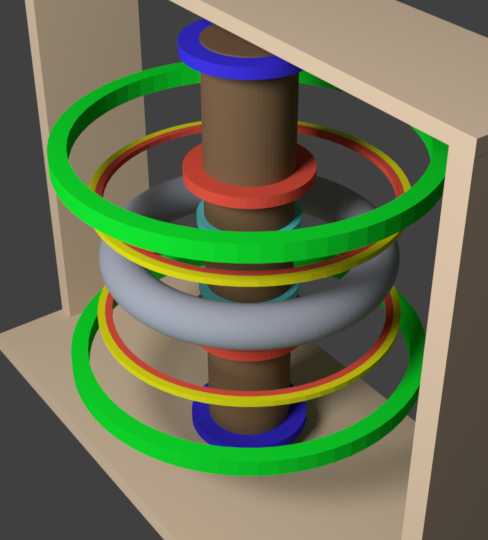
\includegraphics[scale=0.7]{bob2.png}  
\caption{Bobinas tokamak NOVA-FURG - Modelo criado no Blender.}
\label{fig: btokamak}
\end{figure}
\section{Superfícies de fluxo magnético poloidal}
\noindent Uma superfície $S$, onde defini-se um vetor normal, $\bm{n}$, é uma superfície de fluxo de um campo vetorial suave $\bm{B}$ quando
\begin{equation}
\bm{B} \cdot \bm{n}= 0 
\end{equation}
em todos os pontos da superfície $S$, em outras palavras, o campo magnético não atravessa a superfície $S$ em nenhum lugar. 
Então o fluxo magnético que atravessa $S$ é zero. É então possível definir uma função de fluxo escalar $f$ tal que seu valor seja constante na superfície $S$ e
\begin{equation}
\bm{B} \cdot \bm{\nabla} f = 0.
\end{equation}

Para obtermos as superfícies de fluxo do campo magnético poloidal $\bm{B}_{ext}$ gerado pelas bobinas do tokamak NOVA-FURG, foi montada uma tabela de Green, definida e deduzida em \cite[pg. 154]{MagneticControl}, para o campo magnético gerado por cada bobina. 
A tabela de Green para uma bobina, fornece os valores do campo magnético gerado por uma corrente unitária em cada ponto. 
Após gerar as tabelas de Green, para cada bobina, em uma \textit{meshgrid} em coordenadas cartesianas, centrada no centro da secção reta do tokamak NOVA-FURG com uma largura de 63 centímetros e uma altura de 108 centímetros.
Definiu-se a distribuição de campo magnético $\bm{\Psi}(\bm{r})$ como a soma dos valores de cada tabela de Green, em cada $\bm{r}$, multiplicados pela corrente que passa pela mesma.
Chamando a função \textit{contour} do MATLAB para $\bm{\Psi}(\bm{r})$, obtemos a Figura \ref{fig: equipotenc}, onde temos as superfícies de fluxo magnético poloidal gerado pelas bobinas. 
Se adicionarmos a $\bm{\Psi}(\bm{r})$ o campo gerado pela corrente de plasma, obtemos a Figura \ref{fig: equipotenc2}, que mostra as superfícies de fluxo fechadas necessárias para o confinamento do plasma. 
O campo magnético gerado pela corrente de plasma é simulado por 5 bobinas localizadas no centro da secção reta do tokamak NOVA-FURG.
\begin{figure}[H]
\centering
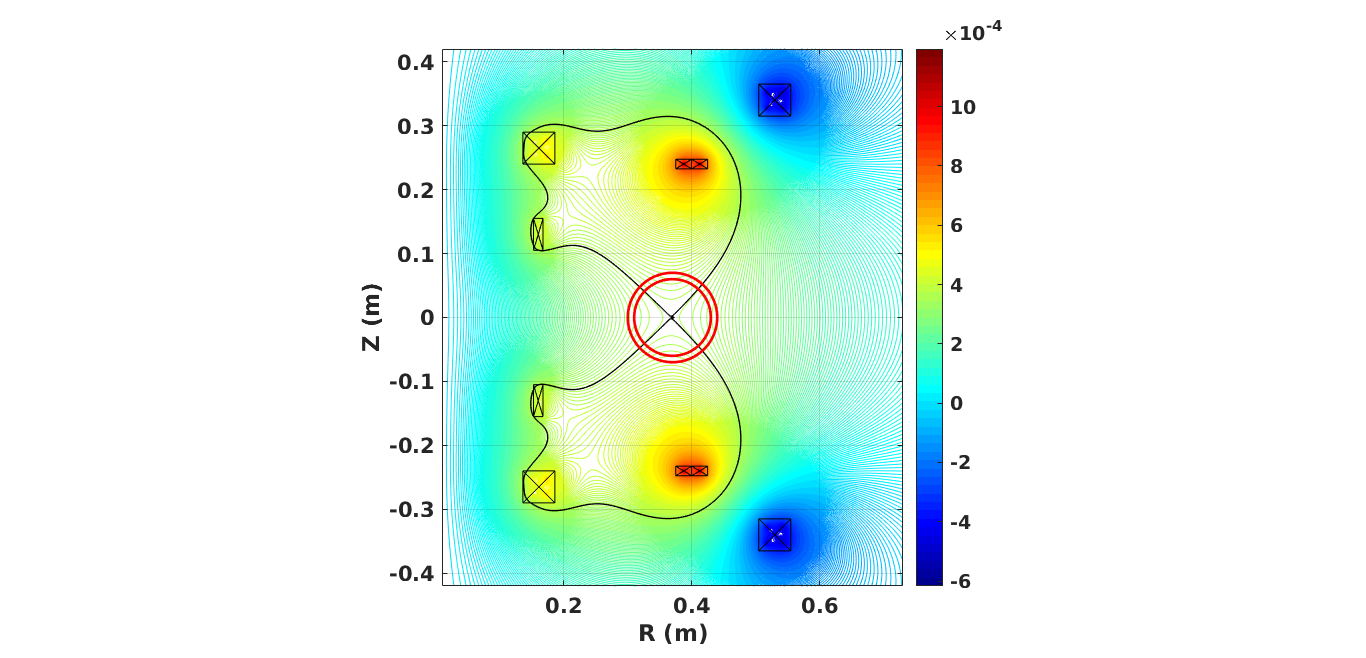
\includegraphics[scale=0.5]{campo001-2.png} 
\caption{Superfícies de fluxo magnético poloidal geradas pelas bobinas do tokamak NOVA-FURG - Imagem feita no MATLAB, com valores de corrente ilustrativos.  Em preto a superfície de fluxo magnético poloidal correspondente a $\bm{\Psi}(\bm{r}_{xp})$, onde $\bm{r}_{xp}=(0.37,0)$ é o ponto-X ($T \cdot m^2$).}
\label{fig: equipotenc}
\end{figure}

\begin{figure}[H]
\centering
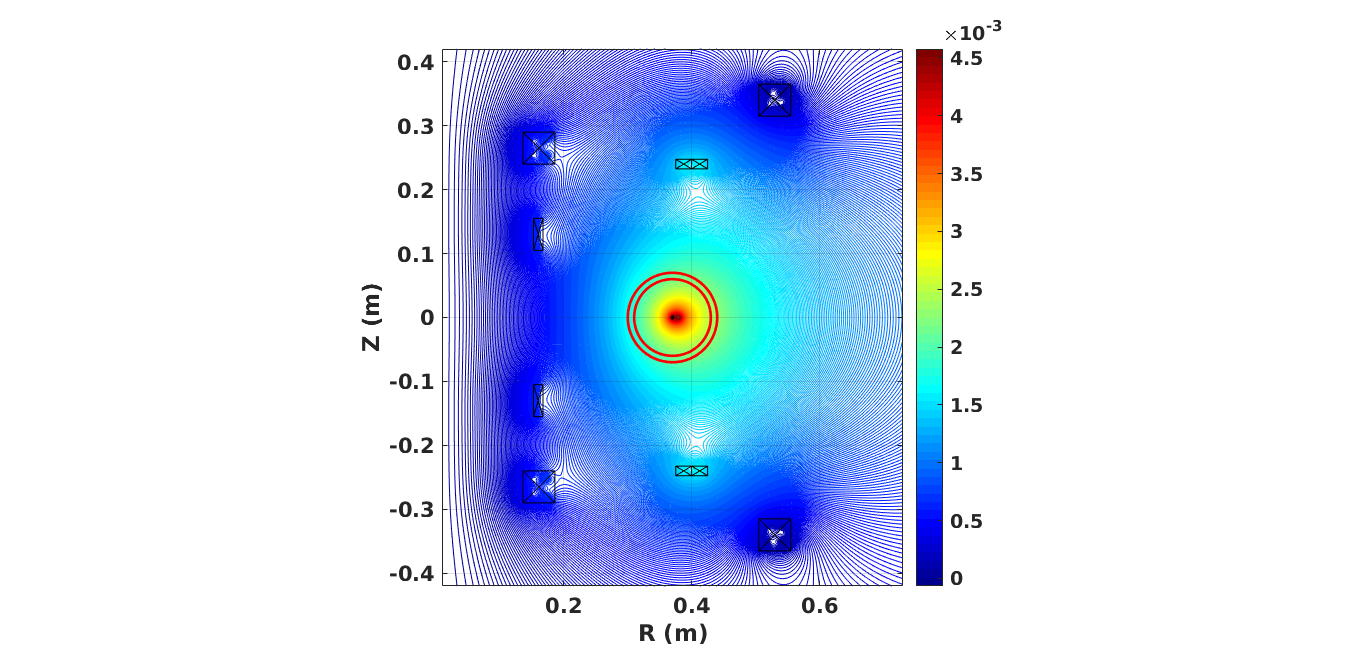
\includegraphics[scale=0.5]{campo002-2.png} 
\caption{Superfícies de fluxo magnético poloidal geradas pelas bobinas com o campo magnético gerado pela corrente de plasma. Imagem feita no MATLAB, com valores de corrente ilustrativos ($T \cdot m^2$).}
\label{fig: equipotenc2}
\end{figure}

\begin{comment}

\begin{figure}[h]
\centering
%\label{fig: equipotenc}
\subfigure[ref1][Sem o campo magnético gerado pela corrente de plasma]{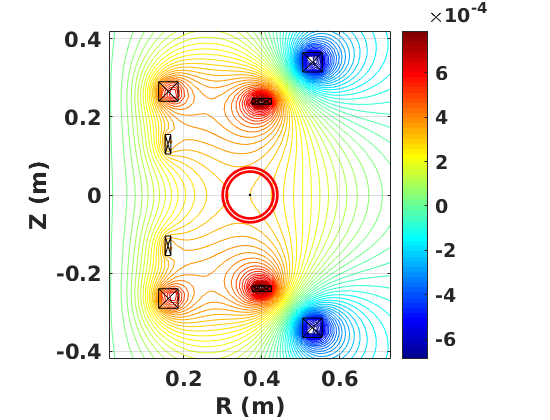
\includegraphics[scale=0.9]{../SImulacao_breakdown/Adaptacao_nova/bacups/campos_1.png} 
\qquad
\subfigure[ref2][Com o campo magnético gerado pela corrente de plasma]{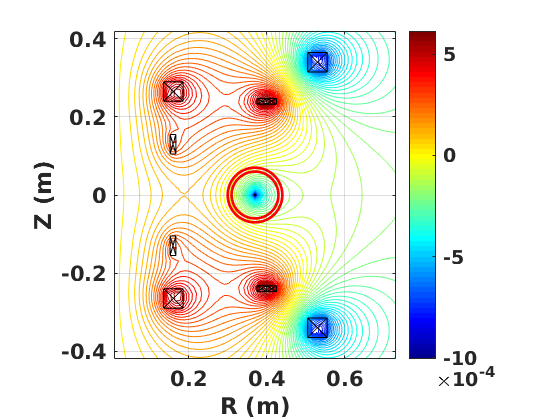
\includegraphics[scale=0.9]{../SImulacao_breakdown/Adaptacao_nova/bacups/campos_2.png} 
\caption{Superfícies de fluxo magnético poloidal geradas pelas bobinas do tokamak NOVA-FURG - Imagem feita no MATLAB, com valores de corrente ilustrativos.}
\end{figure}
\end{comment}

\section{Equações dos campos eletromagnéticos}
\noindent Para simular o modelo desenvolvido no capítulo \ref{faseteorica}, devemos incluir equações para os campos eletromagnéticos. Vamos separar os campos em uma componente gerada pelas correntes que fluem em bobinas fora do plasma e outra causada pelo plasma \cite[cap. 2]{MagneticControl}: $\bm{E} = \bm{E}_{ext} + \bm{E}_{pl}$ e $\bm{B} = \bm{B}_{ext} + \bm{B}_{pl}$. O campo magnético aplicado externamente é produzido por um conjunto de bobinas específicas fora do plasma e possui componentes poloidais e toroidais. O campo toroidal tem uma dependência $1 / R$, enquanto o campo poloidal tem um padrão de quadrupolo,
\begin{equation}
\label{Bext}
\bm{B}_{ext}=\bm{B}_{pol}^{quadrupole}+\frac{R_0B_0}{R}\hat{e}_{\phi} .
\end{equation}
O campo elétrico aplicado externamente é produzido pelo solenoide central do tokamak, que induz uma voltagem de enlaço toroidal, $V_{loop}$. O campo elétrico externo é então dado por
\begin{equation}
\label{Eext}
\bm{E}_{ext} = -\frac{V_{loop}}{2\pi R} \hat{e}_{\phi} .
\end{equation}
O campo eletromagnético gerado pelo plasma é calculado via
\begin{equation}
\nabla^2 \bm{A}_{pl}=-\mu_0\bm{J} 
\end{equation}
onde $\bm{A}_{pl}$ é o potencial vetor magnético devido ao plasma. O campo eletromagnético do plasma então segue de
\begin{equation}
\bm{B}_{pl} = \bm{\nabla} \times \bm{A}_{pl}
\end{equation}
\begin{equation}
\bm{E}_{pl}=-\frac{\partial \bm{A}_{pl}}{\partial t} .
\end{equation}
Os campos eletromagnéticos externos $\bm{E}_{ext}$ e $\bm{B}_{ext}$ são formados antes do plasma e se mantêm constantes. 

\section{Condições iniciais e de contorno}
\noindent As condições iniciais são
$$n = n_0$$
$$J_{\phi}= \frac{n_0 e^2 }{m_e \nu_{eff}} E_{ext,\phi}$$
$$p_e=n_0 k_B T_{e_0}$$
$$p_i=n_0 k_B T_{i_0}, $$
onde $T_{e_0}$ é a temperatura inicial dos elétrons e $\nu_{eff}=\nu_{ei} + \nu_{en} + \nu_{in} + \nu_{loss}$ é a frequência efetiva de colisão dos elétrons. As equações para calcular $\nu_{eff}$ estão no Apêndice \ref{Townsend}, $\nu_{en}$ é atualizado a cada passo temporal por $\nu_{en}=7.89 \times 10^{11} k_B T_{e0}(n_g-n)$, onde $n_g$ é a densidade de partículas neutras inicial, $n_0$ é a densidade inicial de partículas e $p_e$ e $p_i$ são respectivamente pressão cinética eletrônica e iônica. Só teremos campo elétrico na direção toroidal. 
Na borda do domínio computacional temos fixadas as mesmas condições que na condição inicial do interior.
A condição inicial da resistividade e $\nu_{ei}$ é calculada polo código \ref{codigosresitivit} no apêndice \ref{codigos}.
%
\section{Abordagem explícita no tempo}

Na abordagem explícita, foi feita a discretização dos pontos de espaço e de tempo. Usando o método de Euler explícito no tempo para cada EDP, permitiu-se interações onde as não linearidades do modelo não atrapalham, pois estão sempre no tempo $t$ enquanto sempre calculamos o tempo $t+1$. Nas derivadas espaciais foi usada a fórmula das diferenças progressivas $f'(x)=\frac{f(x+1)-f(x)}{h}+o(h)$, onde $o(h)$ é o erro da aproximação.
O sistema foi resolvido modelando a criação e perda de partículas, $\nu_{ion} - \nu_{loss}$, como uma gaussiana $s$,
\begin{equation}
\label{gaussiana}
s = \nu_{ion} - \nu_{loss} = s_0 e^{-\frac{ (x+x_0)^2+y^2 }{\sigma}} ,
\end{equation}
onde $x_0$ é o ponto onde o campo magnético é nulo, $s_0$ e $\sigma$ são constantes para ajustar a curva.
\begin{figure}[H]
\centering
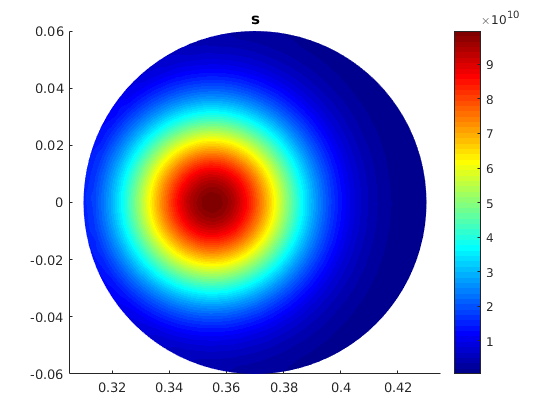
\includegraphics[scale=1]{../SImulacao_breakdown/PDE/sB.png} 
\caption{Gaussiana representando o termo de fonte de partículas ($\nu_{ion} - \nu_{loss}$). Unidade $s^{-1}$ ($s_0=10^{10}$, $x_0=0.015$ e $\sigma=0.001$).}
\label{grafgaussiana}
\end{figure}
%Em $t=0$, quando não estamos usando a aproximação pela gaussiana eq. \ref{gaussiana} sempre temos $\nu_{in} = \nu_{loss} = 0$.
%A \textit{meshgrid} $[x,y]$ representa uma ligação direta entre todos os pontos em cartesianas para os pontos em pseudo-toroidais. 
A \textit{meshgrid} $[x,y]$ foi definida a partir da \textit{meshgrid} em pseudo-toroidais $[R,A]$ por meio da regra obtida na eq. \ref{regrapseudo1} e eq. \ref{regrapseudo2}, assim sendo será necessário usar as expressões de gradiente, divergente, rotacional e laplaciano deduzidas no apêndice \ref{pseudo-toroidaiss}. %, bastará usar as expressões para tais operadores em polares. %Pois todas as contas serão feitas em cartesianas $[x,y]$. %Como $[x,y]$ foi construída a partir das pseudo-toroidais $[R,A]$ que 
Na abordagem explícita, o sistema de coordenadas pseudo-toroidais tem a componente angular $\phi$ desconsiderada, pois assumimos simetria azimutal. 
Portanto tais coordenadas podem ser entendidas como um sistema polar deslocado em $R_0$ da origem. 
Usando coordenadas pseudo-toroidais, ganhamos a vantagem de facilmente introduzir as condições de fronteira do toróide ($r=a_0$). 
Temos o seguinte sistema para ser resolvido
\begin{equation}
\frac{\partial n}{\partial t} = \nu_{ion} - \nu_{loss}+D\nabla^2n + \frac{1}{e} \bm{\nabla} \cdot \bm{J},
\end{equation}
\begin{equation}
\label{momenteletrico} 
\frac{\partial \bm{J}}{\partial t} =  \frac{ne^2}{m_e} \bm{E} -\bm{J}(\nu_{in}+\nu_{en}+\nu_{ion}-\nu_{loss}) -\frac{e}{m_e}\bm{J} \times \bm{B}-\frac{e}{m_e}\bm{\nabla} p_e,
\end{equation}
\begin{equation}
\frac{\partial p_e}{\partial t} = \frac{3}{2}(1+\frac{2 \nu_{en} + \nu_{ion} - \nu_{loss}}{2\nu_{ei}})\eta J^2  -\frac{2ne^2}{m_i} \eta (p_e-p_i),
\end{equation}
\begin{equation}
\frac{\partial p_i}{\partial t} = \frac{2ne^2}{m_i}\eta(p_e-p_i),
\end{equation}
Na simulação explícita deste trabalho assumiremos os campos eletromagnéticos gerados pelo plasma como nulos, pois na fase de \textit{breakdown} a corrente de plasma é pequena. 
Portanto as equações para os campos eletromagnéticos gerados pelo plasma desaparecem.
Na sequência, são apresentadas as figuras \ref{n3}, \ref{j3}, \ref{p3} e \ref{i3} onde temos alguns resultados rodando o código \ref{codigos1}. Com o termo de ionização modelado pela gaussiana da Figura \ref{grafgaussiana}. 


\begin{figure}[H]
\centering
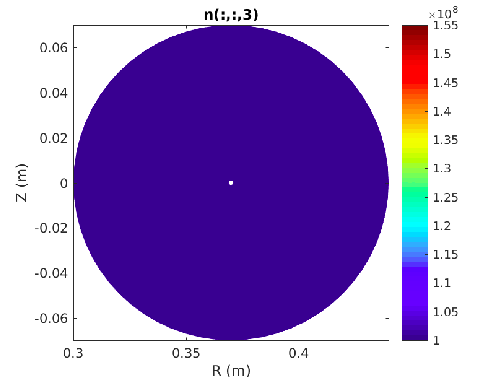
\includegraphics[scale=0.4]{../SImulacao_breakdown/Adaptacao_nova/explicito/n3.png}  
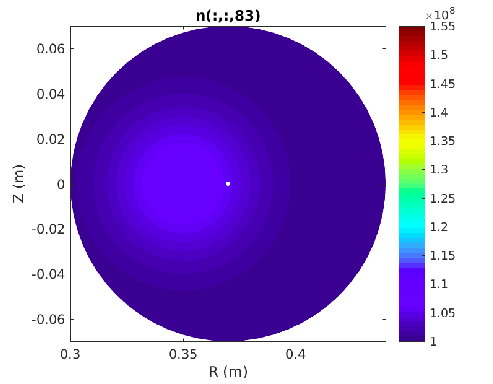
\includegraphics[scale=0.4]{../SImulacao_breakdown/Adaptacao_nova/explicito/n83.png} 
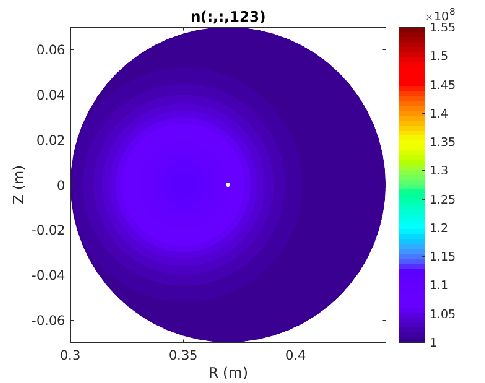
\includegraphics[scale=0.4]{../SImulacao_breakdown/Adaptacao_nova/explicito/n123.png} 
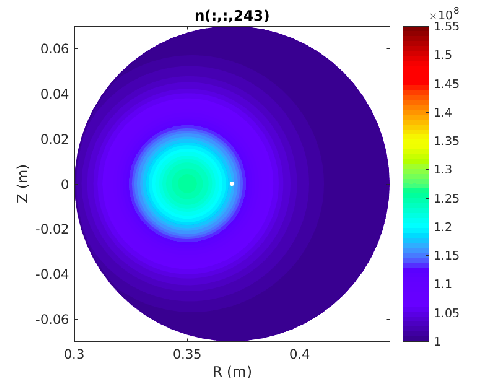
\includegraphics[scale=0.4]{../SImulacao_breakdown/Adaptacao_nova/explicito/n243.png} 
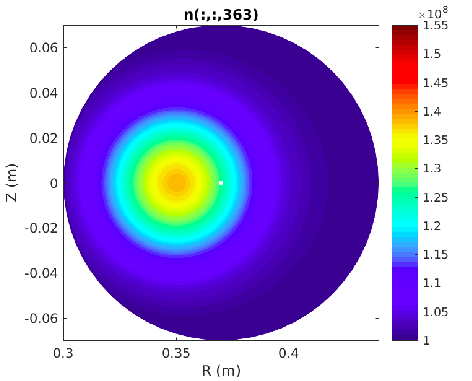
\includegraphics[scale=0.4]{../SImulacao_breakdown/Adaptacao_nova/explicito/n363.png} 
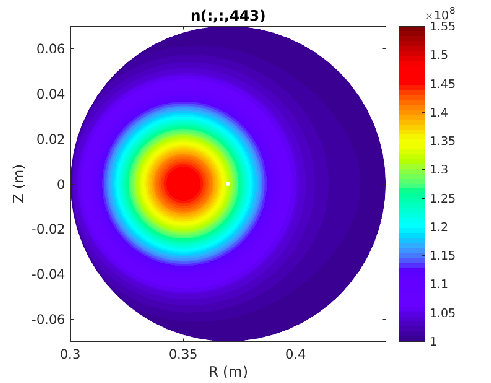
\includegraphics[scale=0.4]{../SImulacao_breakdown/Adaptacao_nova/explicito/n443.png} 
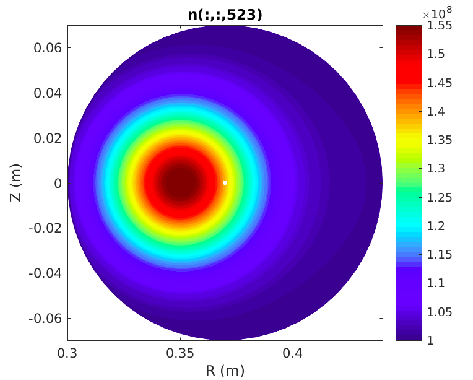
\includegraphics[scale=0.4]{../SImulacao_breakdown/Adaptacao_nova/explicito/n523.png} 
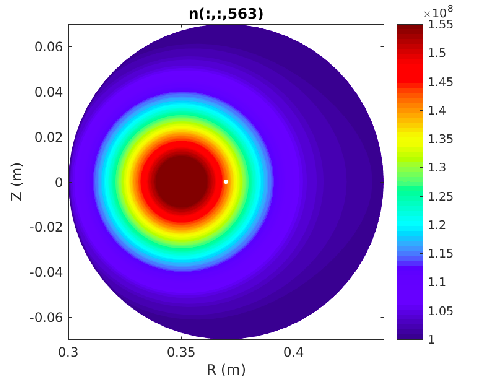
\includegraphics[scale=0.4]{../SImulacao_breakdown/Adaptacao_nova/explicito/n563.png} 
\caption{Densidade de plasma ($m^{-3}$) ($dt=10^{-6}$\ s, $N_g = 65$).}
\label{n3}
\end{figure}
\begin{figure}[H]
\centering
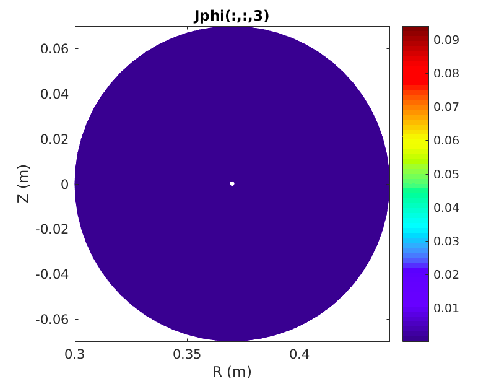
\includegraphics[scale=0.4]{../SImulacao_breakdown/Adaptacao_nova/explicito/j3.png}  
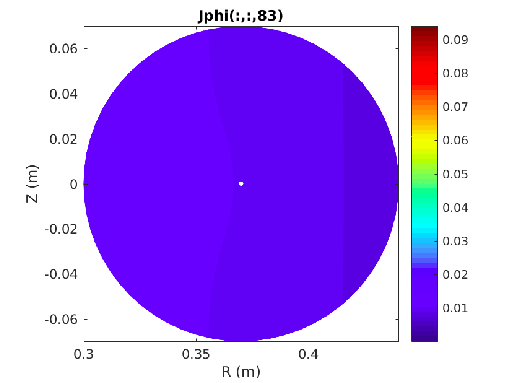
\includegraphics[scale=0.4]{../SImulacao_breakdown/Adaptacao_nova/explicito/j83.png} 
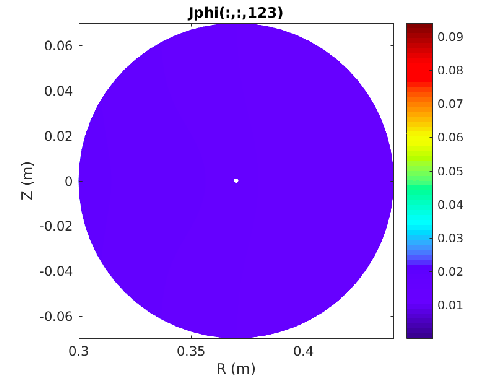
\includegraphics[scale=0.4]{../SImulacao_breakdown/Adaptacao_nova/explicito/j123.png} 
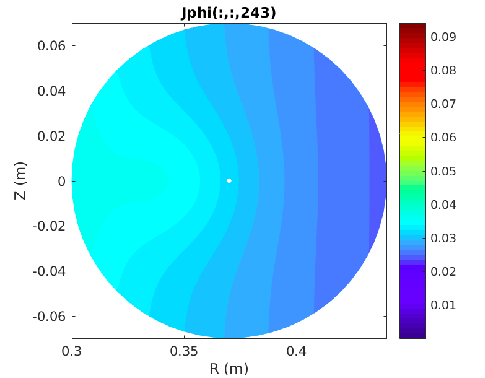
\includegraphics[scale=0.4]{../SImulacao_breakdown/Adaptacao_nova/explicito/j243.png} 
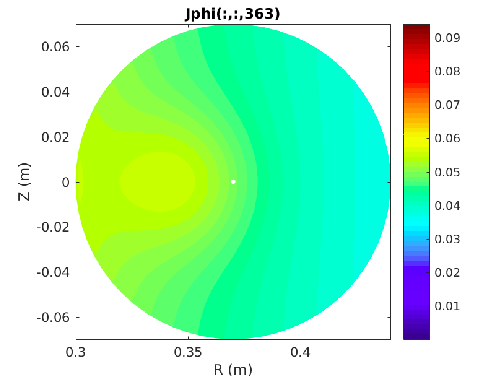
\includegraphics[scale=0.4]{../SImulacao_breakdown/Adaptacao_nova/explicito/j363.png} 
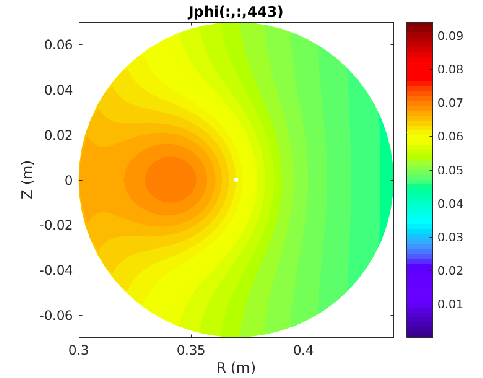
\includegraphics[scale=0.4]{../SImulacao_breakdown/Adaptacao_nova/explicito/j443.png} 
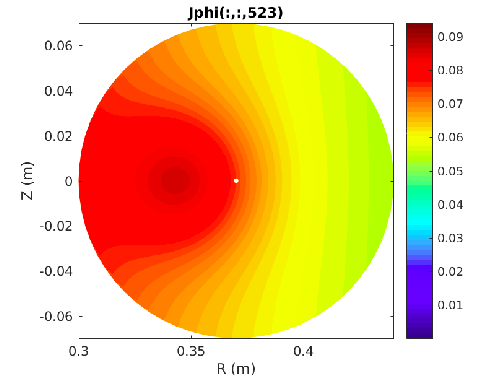
\includegraphics[scale=0.4]{../SImulacao_breakdown/Adaptacao_nova/explicito/j523.png} 
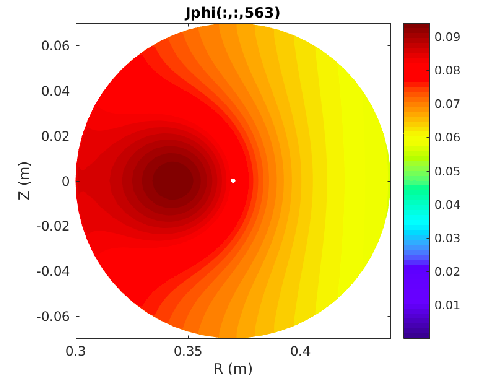
\includegraphics[scale=0.4]{../SImulacao_breakdown/Adaptacao_nova/explicito/j563.png}  
\caption{Componente toroidal da densidade de corrente de plasma ($A/m^2$) ($dt=10^{-6}$\ s, $N_g = 65$).}
\label{j3}
\end{figure}
\begin{figure}[H]
\centering
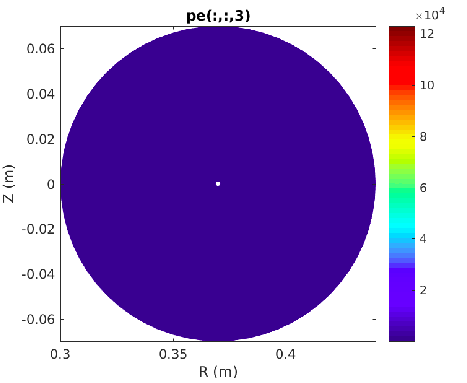
\includegraphics[scale=0.4]{../SImulacao_breakdown/Adaptacao_nova/explicito/p3.png}  
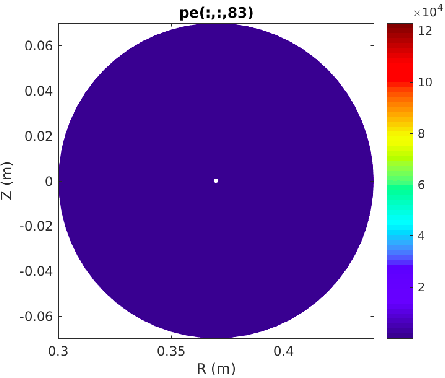
\includegraphics[scale=0.4]{../SImulacao_breakdown/Adaptacao_nova/explicito/p83.png} 
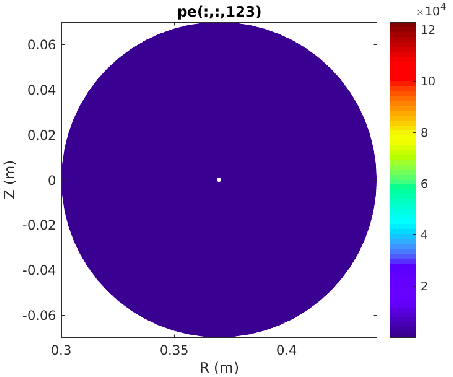
\includegraphics[scale=0.4]{../SImulacao_breakdown/Adaptacao_nova/explicito/p123.png} 
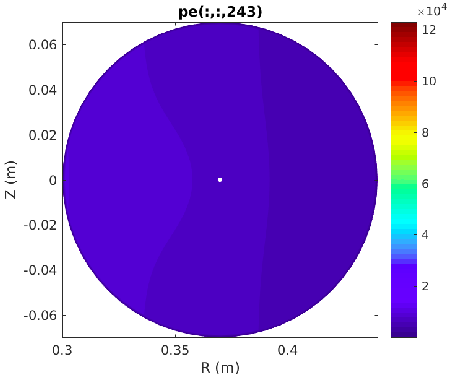
\includegraphics[scale=0.4]{../SImulacao_breakdown/Adaptacao_nova/explicito/p243.png} 
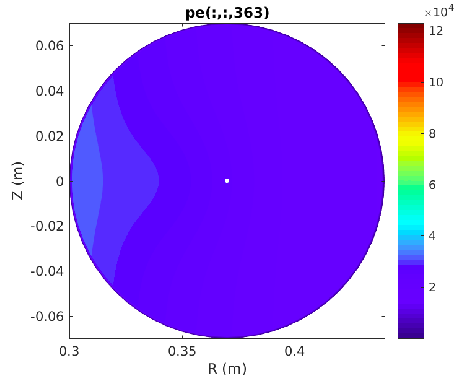
\includegraphics[scale=0.4]{../SImulacao_breakdown/Adaptacao_nova/explicito/p363.png} 
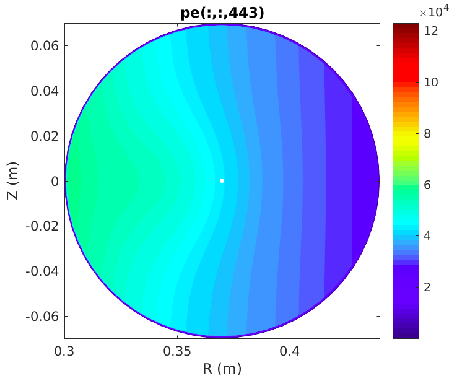
\includegraphics[scale=0.4]{../SImulacao_breakdown/Adaptacao_nova/explicito/p443.png} 
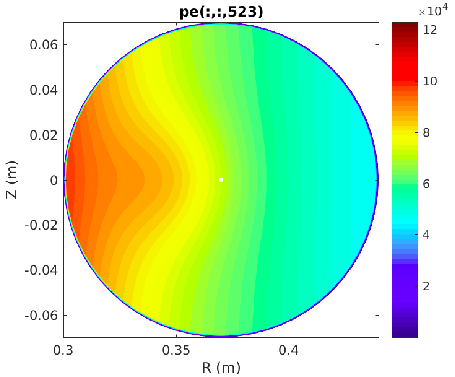
\includegraphics[scale=0.4]{../SImulacao_breakdown/Adaptacao_nova/explicito/p523.png} 
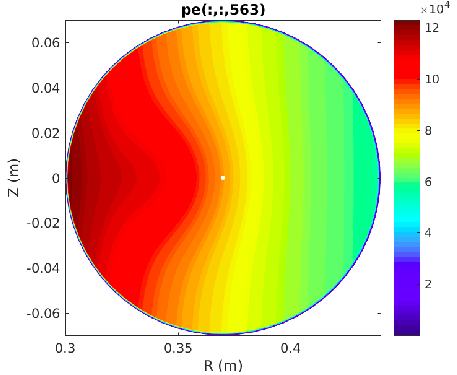
\includegraphics[scale=0.4]{../SImulacao_breakdown/Adaptacao_nova/explicito/p563.png}  
\caption{Pressão eletrônica ($Pa$) ($dt=10^{-6}$\ s, $N_g = 65$).}
\label{p3}
\end{figure}
\begin{figure}[H]
\centering
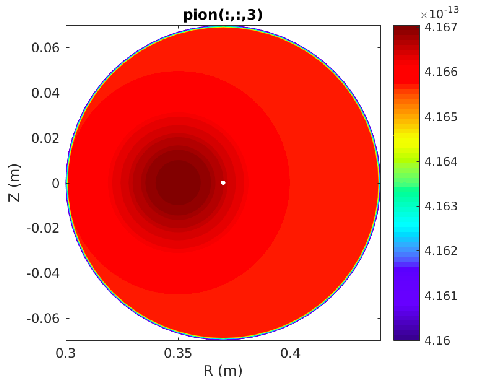
\includegraphics[scale=0.4]{../SImulacao_breakdown/Adaptacao_nova/explicito/i3.png}  
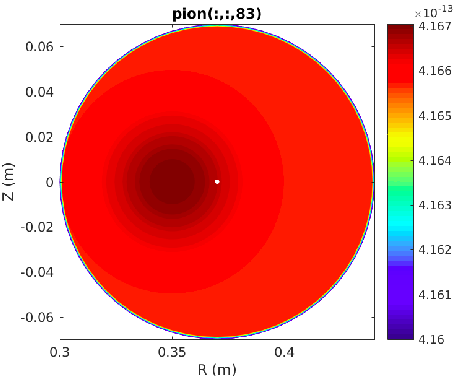
\includegraphics[scale=0.4]{../SImulacao_breakdown/Adaptacao_nova/explicito/i83.png} 
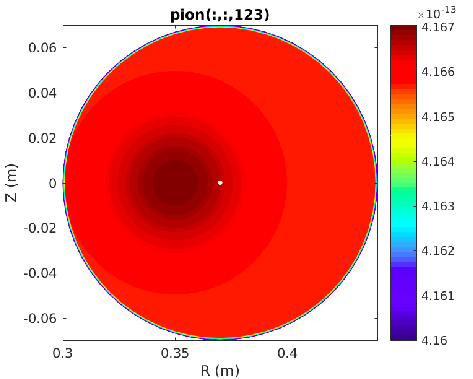
\includegraphics[scale=0.4]{../SImulacao_breakdown/Adaptacao_nova/explicito/i123.png} 
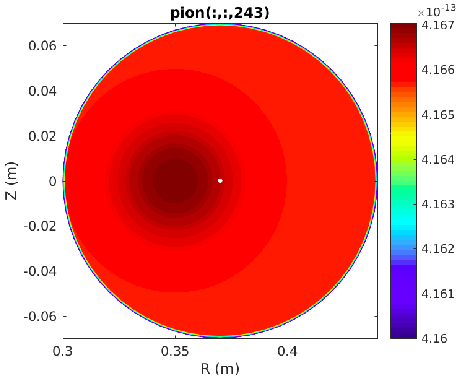
\includegraphics[scale=0.4]{../SImulacao_breakdown/Adaptacao_nova/explicito/i243.png} 
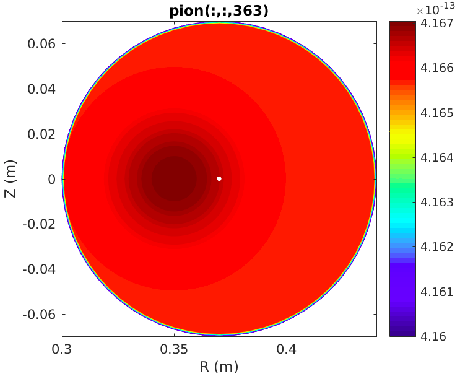
\includegraphics[scale=0.4]{../SImulacao_breakdown/Adaptacao_nova/explicito/i363.png} 
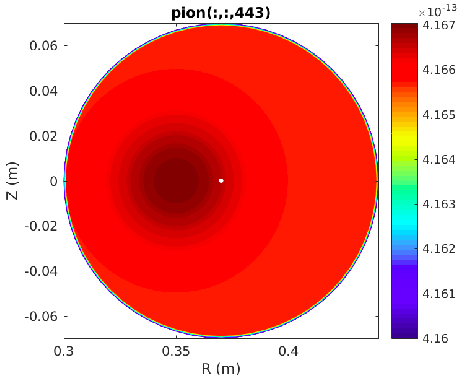
\includegraphics[scale=0.4]{../SImulacao_breakdown/Adaptacao_nova/explicito/i443.png} 
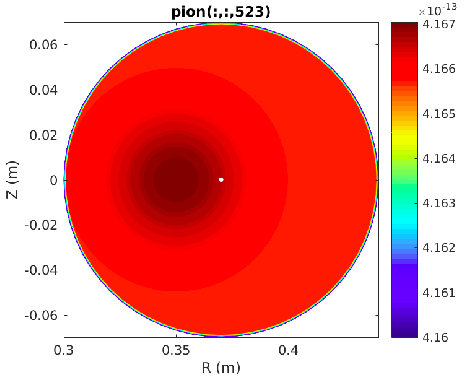
\includegraphics[scale=0.4]{../SImulacao_breakdown/Adaptacao_nova/explicito/i523.png} 
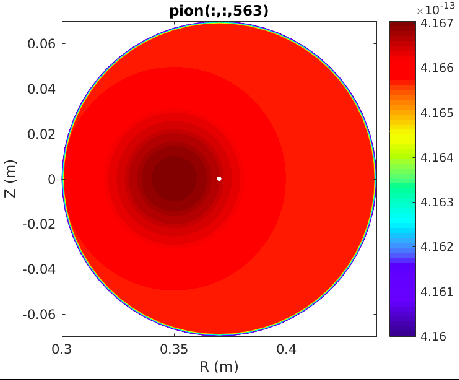
\includegraphics[scale=0.4]{../SImulacao_breakdown/Adaptacao_nova/explicito/i563.png}  
\caption{Pressão iônica ($Pa$) ($dt=10^{-6}$\ s, $N_g = 65$).}
\label{i3}
\end{figure}
 Na Figura \ref{n3} vemos a densidade de plasma aumentando ao longo do tempo, seu ponto de maior valor é o ponto de zero campo magnético localizado em $x_0$.
 Na Figura \ref{j3} notamos que a densidade de corrente em $t=3dt$ está praticamente constante, em $t=243dt$ já está se formando um ponto de máxima densidade de corrente em $x_0$. Já em $t=563dt$, podemos ver claramente o ponto de máxima densidade de corrente em $x_0$.    
 Pela Figura \ref{p3} notamos como a pressão eletrônica tem seus maiores valores onde o campo elétrico externo é mais forte. Em $t=563dt$ já podemos notar a pressão eletrônica subindo no ponto de máxima densidade de plasma. 
Como esperado, podemos ver na Figura \ref{i3} que a pressão iônica sofreu pouca mudança ao longo do tempo.
 %E o fato de estarmos desconsiderando o termo de difusão (laplaciano) na equação da continuidade. 
%Na abordagem explícita foi feita a discretização dos pontos de espaço e de tempo. Então para cada equação é feito um cálculo da derivada pela diferença do tempo atual e o tempo seguinte dividido pelo intervalo de tempo $dt$. Isto pode ser rearranjado de forma a permitir uma iteração onde as não linearidades do modelo não atrapalham, pois estão sempre no tempo $t$ enquanto sempre calculamos o tempo $t+1$. 

\section{Abordagem pelo PDE Solver}

\subsection{Introdução ao PDE Solver}
\noindent O sistema de equações diferenciais parciais (EDPs) a ser resolvido pelo PDE solver deve estar no formato, 
\begin{equation}
\bm{m} \frac{\partial^2 \bm{u}}{\partial t^2} + \bm{d} \frac{\partial \bm{u}}{\partial t} - \bm{\nabla} \cdot \left( \bm{c} \bm{\nabla} \bm{u} \right) + \bm{a}\bm{u} = \bm{f}.
\label{sistemapde}
\end{equation} 
onde o domínio da solução pode ser de qualquer formato. Neste trabalho o domínio será circular, com raio $a_0$ e deslocado em $R_0$ a direita da origem. O PDE Solver aceita apenas problemas escritos em cartesianas. Por esta razão as equações que estão escritas em coordenadas cilíndricas devem sofrer uma mudança de coordenadas a fim de ficarem no formato de coordenadas cartesianas.
Neste trabalho, $\bm{u}=[n, J_\phi, p_e, p_i]$. As densidades de corrente poloidais, $J_r$ e $J_z$, são assumidas como iguais 0.

Vamos mostrar um exemplo onde um modelo 3-D pode ser analisado usando um modelo 2-D por ser axissimétrico. 
A geometria do modelo, as propriedades do material e as condições de contorno devem ser simétricas em relação a um único eixo para que essa simplificação de 3-D para 2-D seja apropriada. 
Devido a essa simetria, um sistema de coordenadas cilíndricas é a forma mais conveniente para definir a equação diferencial parcial. 
No entanto, o PDE Solver espera as equações em um sistema cartesiano. 
Um dos principais objetivos deste exemplo é mostrar como expressar as EDPs que formam nosso modelo em coordenadas cartesiana de modo que o PDE Solver possa resolve-las adequadamente.
Este exemplo em particular mostra a transferência de calor em uma haste com um corte circular transversal. Existe uma fonte de calor na extremidade esquerda da haste e uma temperatura fixa na extremidade direita. 
A superfície externa da haste troca calor com o ambiente devido à convecção. 
Além disso, o calor é gerado dentro da haste devido à deterioração radioativa.
Gostaríamos de calcular a temperatura na haste em função
de tempo. 
A equação parabólica que descreve a transferência de calor é
$$ \rho C \frac{\partial u}{\partial t} - \nabla \cdot (k \nabla u) = q$$
onde $\rho, C, $ e $k$ são a densidade, calor específico, e a condutividade térmica do material, $u$ é a temperatura, e
$q$ é o calor gerado na haste. Como o problema é axissimétrico, é conveniente escrever este
equação em um sistema de coordenadas cilíndricas,
$$ \rho C \frac{\partial u}{\partial t} - 
\frac{1}{r}\frac{\partial}{\partial r}\left(kr\frac{\partial u}{\partial r}\right)
- \frac{1}{r^2}\frac{\partial}{\partial \phi}\left(k\frac{\partial u}{\partial\phi}\right)
- \frac{\partial}{\partial z}\left(k\frac{\partial u}{\partial z}\right)
= q,
$$
%onde $r, \phi$, e $z$ são as variáveis do sistema de coordenadas cilíndricas. 
Como o problema é axissimétrico, $\partial u/\partial\phi = 0$, e multiplicando por $r$ a equação é reescrita como
$$ r\rho C \frac{\partial u}{\partial t} -
\frac{\partial}{\partial r}\left(kr\frac{\partial u}{\partial r}\right)
- \frac{\partial}{\partial z}\left(kr\frac{\partial u}{\partial z}\right)
= rq.
$$ 
Esta equação pode ser convertida no formato suportado pelo PDE Solver se $ r $ for definido como $ x $ e $ z $ for definido como $ y $. Reescrevendo a equação acima, obtêm-se
$$ 
\rho Cx\frac{\partial u}{\partial t}
-\nabla\cdot(kx\nabla u) = qx.
$$

Para repetir a transformação do exemplo acima com o modelo de dois fluidos, primeiro expandimos o sistema com os operadores em cilíndricas, %O $\phi$ é o ângulo na direção toroidal e nas direções poloidais temos $r$ sendo a direção radial e $z$ sendo a direção vertical.
\begin{equation}
\frac{\partial n}{\partial t} = \nu_{ion} - \nu_{loss}+D \left[  \frac{\partial^2 n}{\partial r^2} + \frac{1}{r} \frac{\partial n}{\partial r} + \frac{1}{r^2} \frac{\partial^2 n}{\partial \phi^2}  + \frac{\partial^2 n}{\partial z^2} \right] + 
\end{equation}
\begin{equation}
\frac{1}{e}  \left[ \frac{1}{r}  \frac{\partial }{\partial r}\Big(r J_r\Big) + \frac{1}{r} \frac{\partial J_\phi}{\partial \phi} +  \frac{\partial J_z}{\partial z} \right] .
\end{equation}
Como $J_r$ e $J_z$ são assumidos nulos, e como assumimos simetria azimutal temos $\frac{\partial \bm{J}_\phi}{\partial \phi} = 0$ e $ \frac{1}{r^2} \frac{\partial^2 n}{\partial \phi^2}=0$, ou seja, o termo $\bm{\nabla} \cdot \bm{J}$ desaparece, resultando em
\begin{equation}
\frac{\partial n}{\partial t} = \nu_{ion} - \nu_{loss}+D \left[  \frac{\partial^2 n}{\partial r^2} + \frac{1}{r} \frac{\partial n}{\partial r}  + \frac{\partial^2 n}{\partial z^2} \right] .
\end{equation}
A equação de conservação do momento eletrônico, usando a simetria  $\frac{1}{r} \frac{\partial p_e}{\partial \phi}  = 0$ fica
\begin{equation}
\label{momenteletrico1} 
\frac{\partial \bm{J}}{\partial t} =  \frac{ne^2}{m_e} \bm{E} -\bm{J}(\nu_{in}+\nu_{en}+\nu_{ion}-\nu_{loss}) -\frac{e}{m_e}\bm{J} \times \bm{B}+\frac{e}{m_e} \left[ \frac{\partial p_e}{\partial r} \hat{e}_r + \frac{\partial p_e}{\partial z} \hat{e}_z \right] .
\end{equation}
E as equações para os campos gerados pelo plasma, onde $\nabla^2 \bm{A}_{pl}=-\mu_0\bm{J}$, $ \bm{B}_{pl} = \bm{\nabla} \times \bm{A}_{pl}$ e $\bm{E}_{pl}=-\frac{\partial \bm{A}_{pl}}{\partial t} $, ficam% lembrando que $\frac{\partial \bm{B}_{pl_r,\phi,z}}{\partial \phi} = \frac{\partial \bm{E}_{pl_r,\phi,z}}{\partial \phi} = 0$ ficam

\begin{equation}
\frac{1}{r}  \frac{\partial}{\partial r} \big( r E_{pl_r} \big) +  \frac{\partial E_{pl_z}}{\partial z}   = \frac{r}{\epsilon_0},
\end{equation}
\begin{equation}
\left[- \frac{\partial E_{pl_\phi}}{\partial z} \right]  \hat{e}_r + \left[  \frac{\partial E_{pl_r}}{\partial z} -  \frac{\partial E_{pl_z}}{\partial r}  \right] \hat{e}_\phi + \left[ \frac{1}{r} \frac{\partial}{\partial r} \big( r E_{pl_\phi} \big)  \right] \hat{e}_z = -\frac{\partial \bm{B}_{pl}}{\partial t},
\end{equation}
\begin{equation}
\left[ - \frac{\partial B_{pl_\phi}}{\partial z} \right]  \hat{e}_r + \left[  \frac{\partial B_{pl_r}}{\partial z} -  \frac{\partial B_{pl_z}}{\partial r}  \right] \hat{e}_\phi + \left[ \frac{1}{r} \frac{\partial}{\partial r} \big( r B_{pl_\phi} \big) \right] \hat{e}_z = \mu_0 (\bm{J} + \epsilon_0 \frac{\partial \bm{E}_{pl}}{\partial t} ) .
\end{equation}
O sistema que será implementado é
\begin{equation}
\label{contfinal} 
\frac{\partial n}{\partial t} = \nu_{ion} - \nu_{loss}+D \left[  \frac{\partial^2 n}{\partial r^2} + \frac{1}{r} \frac{\partial n}{\partial r}  + \frac{\partial^2 n}{\partial z^2} \right] ,
\end{equation}
\begin{equation}
\frac{\partial \bm{J}}{\partial t} =  \frac{ne^2}{m_e} \bm{E} -\bm{J}(\nu_{in}+\nu_{en}+\nu_{ion}-\nu_{loss}) -\frac{e}{m_e}\bm{J} \times \bm{B}+\frac{e}{m_e} \left[ \frac{\partial p_e}{\partial r} \hat{e}_r + \frac{\partial p_e}{\partial z} \hat{e}_z \right],
\end{equation}
\begin{equation}
\frac{\partial p_e}{\partial t} = \frac{3}{2}(1+\frac{2 \nu_{en} + \nu_{ion} - \nu_{loss}}{2\nu_{ei}})\eta J^2  -\frac{2ne^2}{m_i} \eta (p_e-p_i),
\end{equation}
\begin{equation}
\frac{\partial p_i}{\partial t} = \frac{2ne^2}{m_i}\eta(p_e-p_i) .
\end{equation}
Agora multiplica-se a eq. \ref{contfinal} pela coordenada radial $r$  e obtêm-se
\begin{equation}
r \frac{\partial n}{\partial t} = r ( \nu_{ion} - \nu_{loss} ) +D \left[ r  \frac{\partial^2 n}{\partial r^2} +  \frac{\partial n}{\partial r}  + r \frac{\partial^2 n}{\partial z^2} \right] 
\end{equation}
rearranjando
\begin{equation}
r \frac{\partial n}{\partial t} = r ( \nu_{ion} - \nu_{loss} ) + \frac{\partial}{\partial r}\left(r D \frac{\partial n}{\partial r}\right)
+ \frac{\partial}{\partial z}\left(r D \frac{\partial n}{\partial z}\right) .
\end{equation}
Renomeando $r$ como $x$ e $z$ como $y$, temos que
\begin{equation}
x \frac{\partial n}{\partial t} = x ( \nu_{ion} - \nu_{loss} ) + \frac{\partial}{\partial x}\left(x D \frac{\partial n}{\partial x}\right)
+ \frac{\partial}{\partial y}\left(x D \frac{\partial n}{\partial y}\right) .
\end{equation}
De acordo com a eq. \ref{sistemapde}, 
\begin{equation}
0 \frac{\partial^2 n}{\partial t^2} +  x \frac{\partial n}{\partial t} - \nabla \cdot \left( x D \nabla n \right) + 0 n = x ( \nu_{ion} - \nu_{loss} ) 
\end{equation}
e por fim
\begin{equation}
x \frac{\partial n}{\partial t} - \nabla \cdot \left( x D \nabla n \right) = x ( \nu_{ion} - \nu_{loss} ) .
\end{equation}
Para as demais equações basta manter a definição de $r$ para $x$ e $z$ para $y$
\begin{equation}
\frac{\partial \bm{J}}{\partial t} =  \frac{ne^2}{m_e} \bm{E} -\bm{J}(\nu_{in}+\nu_{en}+\nu_{ion}-\nu_{loss}) -\frac{e}{m_e}\bm{J} \times \bm{B}+\frac{e}{m_e} \left[ \frac{\partial p_e}{\partial y} \hat{e}_y + \frac{\partial p_e}{\partial x} \hat{e}_x \right],
\end{equation}
\begin{equation}
\frac{\partial p_e}{\partial t} = \frac{3}{2}(1+\frac{2 \nu_{en} + \nu_{ion} - \nu_{loss}}{2\nu_{ei}})\eta J^2  -\frac{2ne^2}{m_i} \eta (p_e-p_i),
\end{equation}
\begin{equation}
\frac{\partial p_i}{\partial t} = \frac{2ne^2}{m_i}\eta(p_e-p_i) .
\end{equation}
Lembrando que a única componente de $\bm{J}$ que iremos calcular é a componente toroidal. Por hora iremos considerar a quantidade $\frac{e}{m_e}J_\phi  B_\phi=0$ uma vez que no início do plasma $J_\phi \approx 10^{-10}$ A/$m^2$. Também iremos desconsiderar o termo $\left[ \frac{\partial p_e}{\partial y} \hat{e}_y + \frac{\partial p_e}{\partial x} \hat{e}_x \right]$ por ser desprezível durante a fase de \textit{breakdown}. Então, o sistema de equações a ser resolvido, no formato da eq. \ref{sistemapde} fica
\begin{equation}
x \frac{\partial n}{\partial t} - \nabla \cdot \left( x D \nabla n \right) = x ( \nu_{ion} - \nu_{loss} ) ,
\end{equation}
\begin{equation}
\frac{\partial J_\phi}{\partial t} +(\nu_{in}+\nu_{en}+\nu_{ion}-\nu_{loss}) J_\phi =  \frac{ne^2}{m_e} \bm{E} ,
\end{equation}
\begin{equation}
\frac{\partial p_e}{\partial t} + \frac{2ne^2}{m_i} \eta p_e = \frac{3}{2}(1+\frac{2 \nu_{en} + \nu_{ion} - \nu_{loss}}{2\nu_{ei}})\eta |J_\phi|  +\frac{2ne^2}{m_i} \eta p_i,
\end{equation}
\begin{equation}
\frac{\partial p_i}{\partial t} + \frac{2ne^2}{m_i} \eta p_i = \frac{2ne^2}{m_i}\eta p_e .
\end{equation}
No formato matricial
%\bm{A}
\begin{displaymath}
\left(\begin{array}{c}
x \\
0\\
1\\
1
\end{array}\right)
\left(\begin{array}{c}
\frac{\partial n}{\partial t}\\
\frac{\partial J_\phi}{\partial t}\\
\frac{\partial p_e}{\partial t}\\
\frac{\partial p_i}{\partial t}
\end{array}\right) - \bm{\nabla} \cdot \left( \left(\begin{array}{c}
x D\\
0\\
0\\
0
\end{array}\right) \bm{\nabla} \left(\begin{array}{c}
n\\
J_\phi\\
p_e\\
p_i
\end{array}\right) \right) + \left(\begin{array}{c}
0\\
(\nu_{in}+\nu_{en}+\nu_{ion}-\nu_{loss})\\
\frac{2ne^2}{m_i} \eta\\
\frac{2ne^2}{m_i} \eta
\end{array}\right)\left(\begin{array}{c}
n\\
J_\phi\\
p_e\\
p_i
\end{array}\right) =
\end{displaymath}
\begin{displaymath}
= \left(\begin{array}{c}
x ( \nu_{ion} - \nu_{loss} )\\
\frac{ne^2}{m_e} \bm{E} \\
\frac{3}{2}(1+\frac{2 \nu_{en} + \nu_{ion} - \nu_{loss}}{2\nu_{ei}})\eta |J_\phi|  +\frac{2ne^2}{m_i} \eta p_e\\
\frac{2ne^2}{m_i}\eta p_e
\end{array}\right).
\end{displaymath}

Para fazer as simulações pelo PDE Solver os coeficientes terão a forma de vetores coluna, sendo cada um com quatro elementos: um para cada equação ($n$, $J_\phi$, $p_e$, $p_i$). Aqui $\bm{m}$ é nulo, o coeficiente $\bm{d}$ é calculado com o código \ref{codigosd}, o coeficiente $\bm{c}$ é calculado com o código \ref{codigosc}, o coeficiente $\bm{a}$ é calculado com o código \ref{codigosa} e o coeficiente $\bm{f}$ é calculado com o código \ref{codigosf}. Nas próximas  secções veremos os resultados destas simulações.

Os campos externos elétrico $\bm{E}_{ext}$ e magnético $\bm{B}_{ext}$ são calculados pelas eq. \ref{Eext} e eq. \ref{Bext}, e precisam ser interpolados para a malha da Figura \ref{triangmesh}. Para isso foram criados os  códigos \ref{codigoscampo} e \ref{codigosreg}, que fazem a interpolação e em seguida regulam o tamanho de cada campo para cada etapa da resolução.
Para a condição de contorno, chamamos o código \ref{codigosini} para os pontos da borda. Para as condições iniciais chamamos para os demais pontos. A malha triangular usada é Figura \ref{triangmesh}, onde $H_{max}$ define o refinamento da malha.
\begin{figure}[H]
\centering
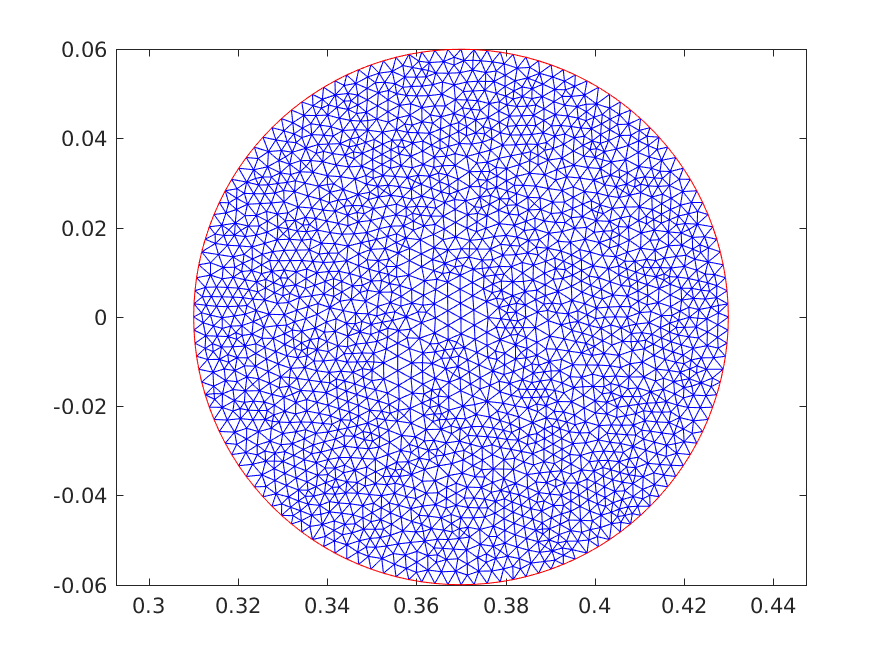
\includegraphics[scale=1]{../SImulacao_breakdown/PDE/malha.png}  
\caption{Malha triangular com $H_{max}=0.006$.}
\label{triangmesh}
\end{figure}
\subsection{Aproximação da ionização por uma gaussiana}
\label{pdesolvergauss}
\noindent Na primeira simulação realizada pelo código usando o PDE Solver, iremos modelar a criação e perda de partículas por uma gaussiana, eq. \ref{gaussiana}. %com gráfico na Figura \ref{grafgaussiana} e $s_0=10^{11}$, $x_0=0$ e $\sigma=0.001$. 
Para resolvermos o modelo é rodado o código \ref{codigos7}, com os valores $s_0=10^{11}$, $x_0=0$ e $\sigma=0.001$ para a gaussiana. 
Os resultados obtidos, são então apresentados nas figuras \ref{densidadeB}, \ref{densidadeCB}, \ref{pressaoB} e \ref{pressao2B}. 
Plotagem em termos de proporção, ou seja plotamos o valor da variável macroscópica dividido pela condição inicial.
\begin{figure}[H]
\centering
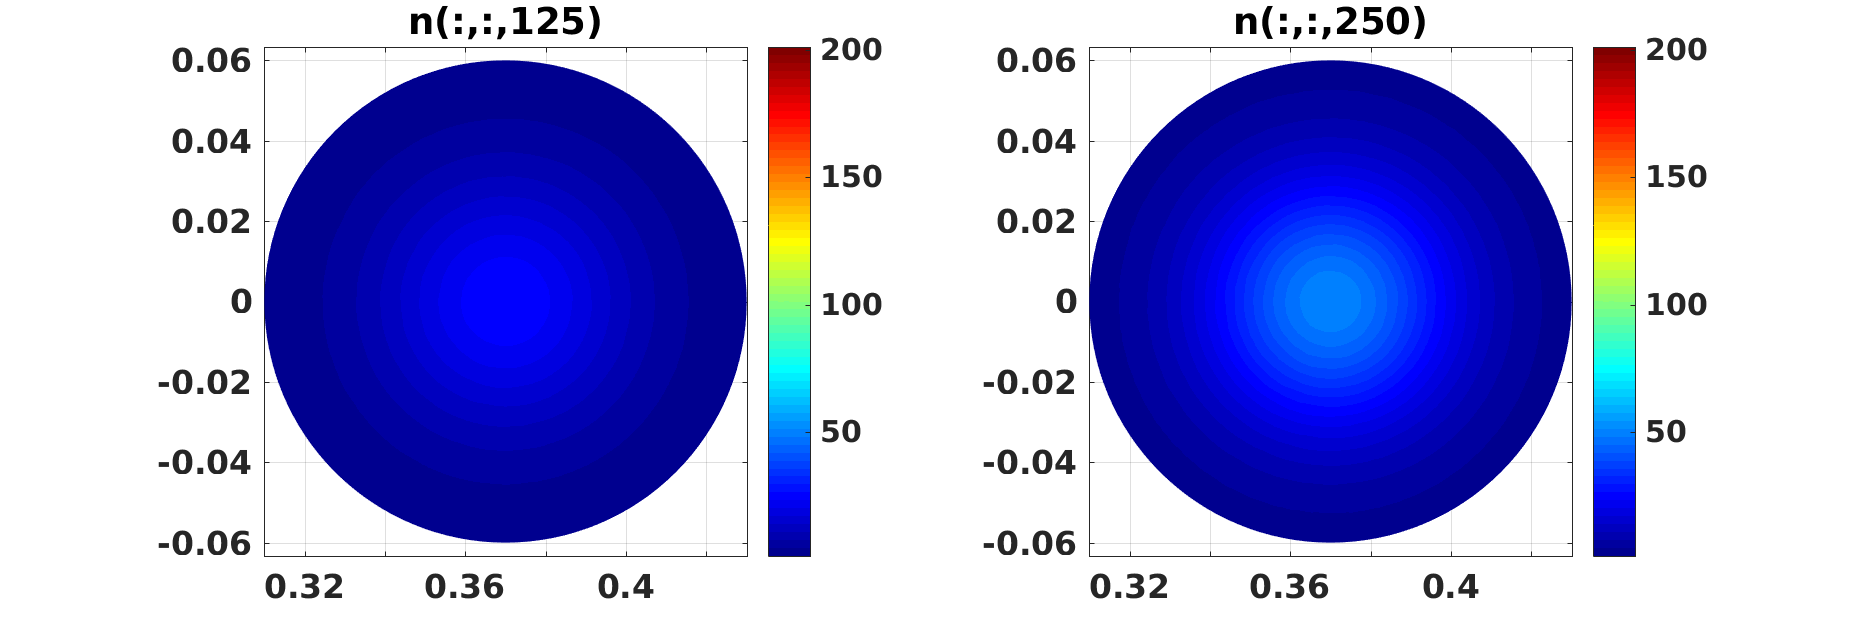
\includegraphics[scale=0.5]{../SImulacao_breakdown/PDE/ntod1B6.png}  
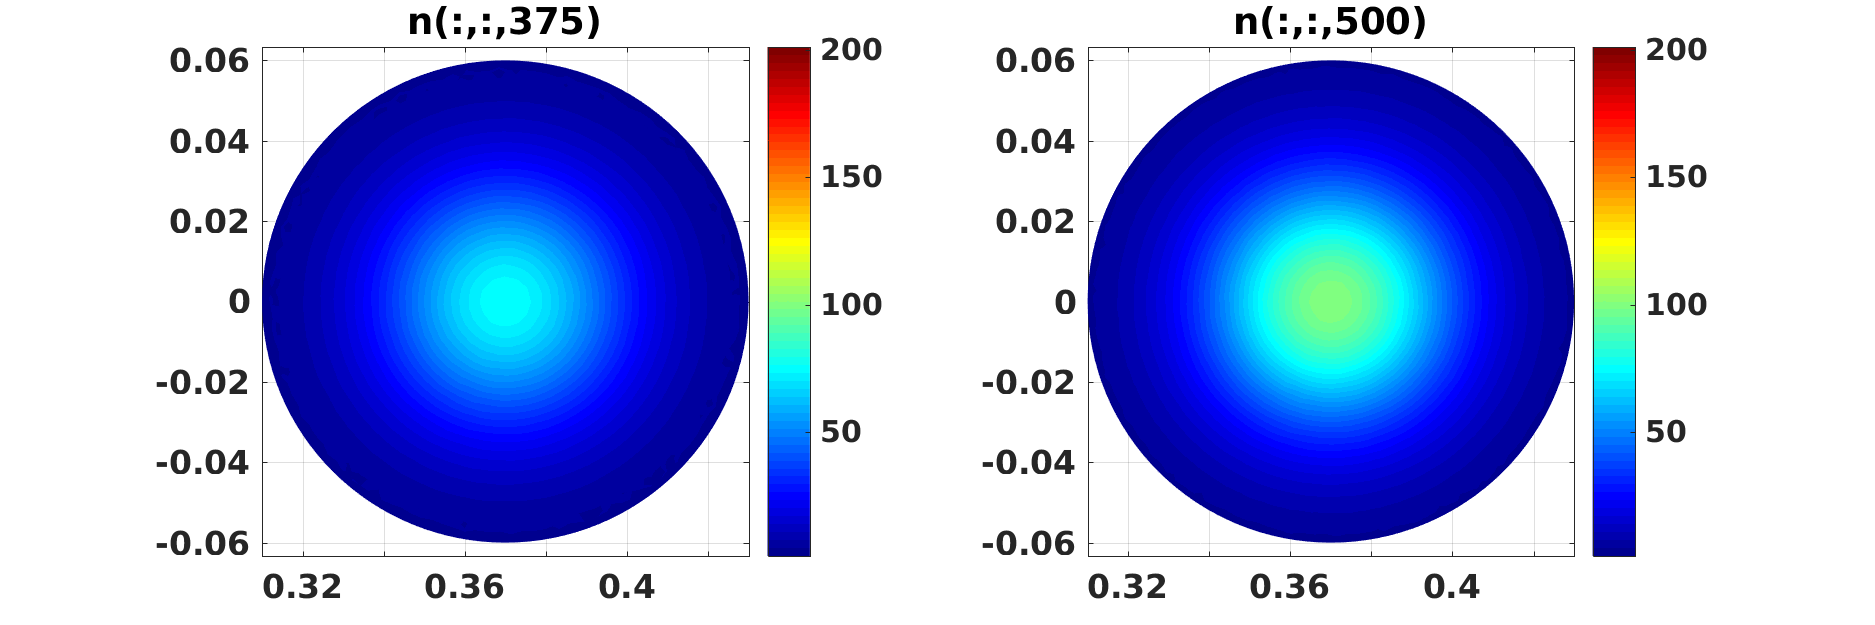
\includegraphics[scale=0.5]{../SImulacao_breakdown/PDE/ntod2B6.png} 
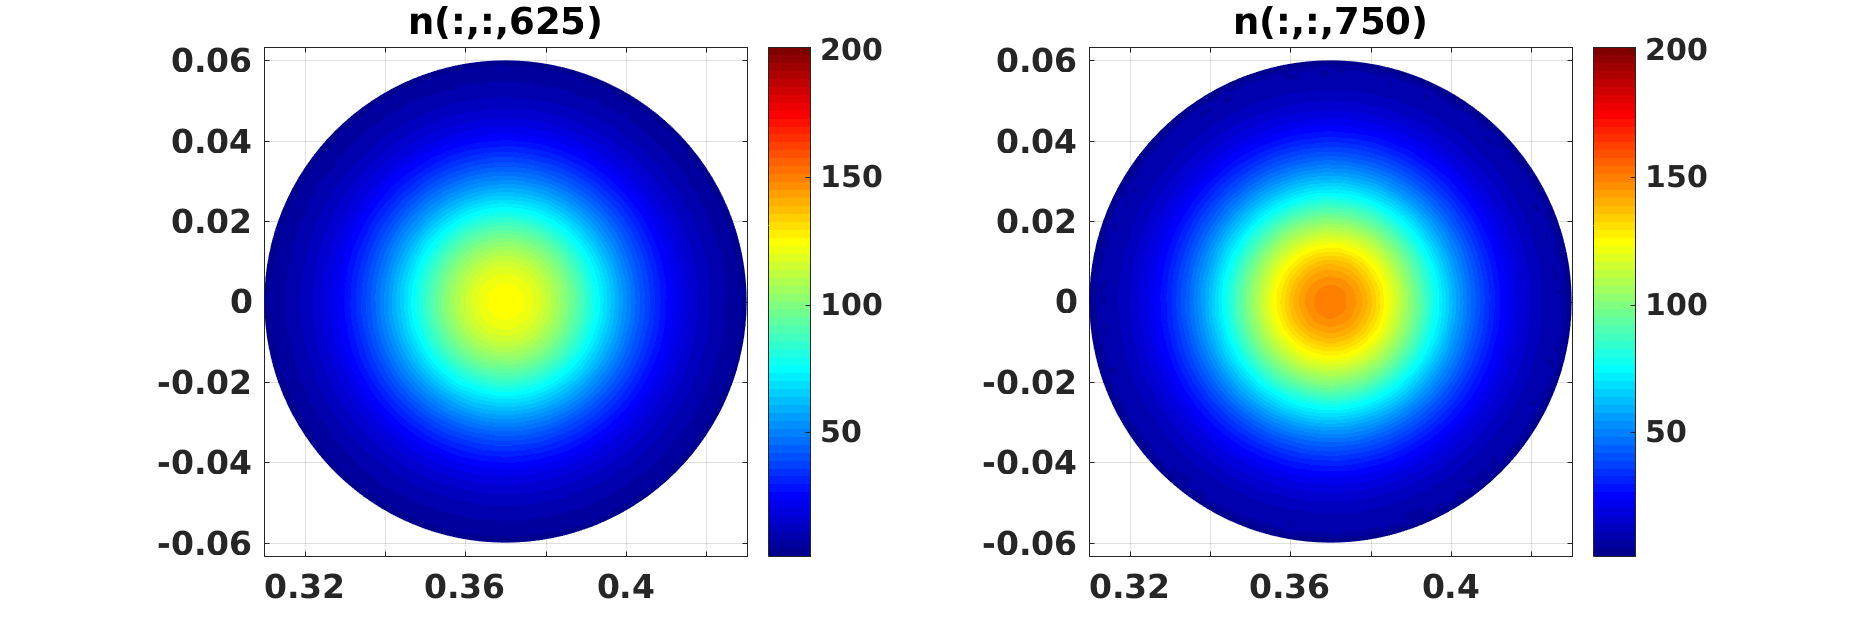
\includegraphics[scale=0.5]{../SImulacao_breakdown/PDE/ntod3B6.png} 
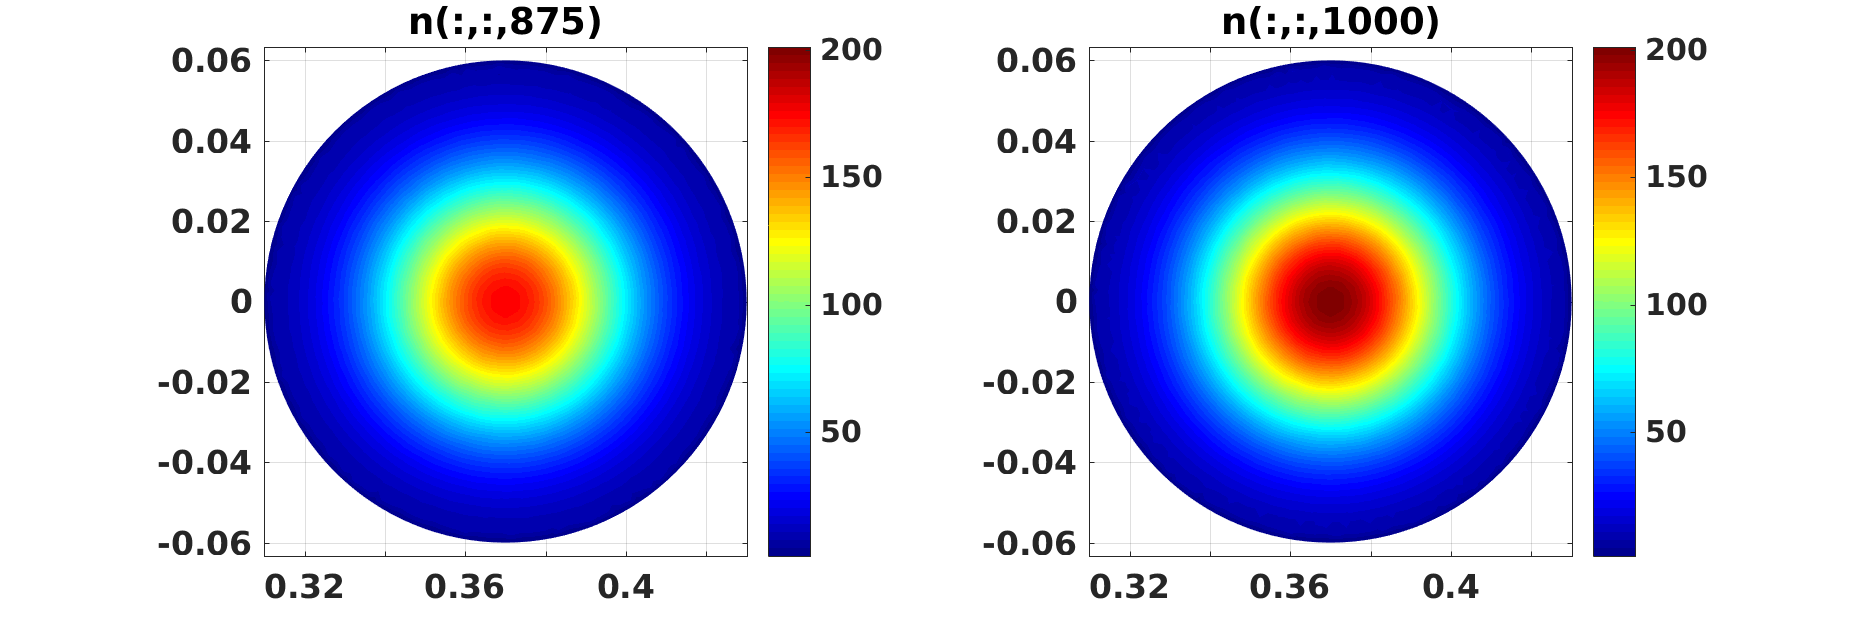
\includegraphics[scale=0.5]{../SImulacao_breakdown/PDE/ntod4B6.png} 
\caption{Densidade de plasma ($m^{-3}$), aproximação da ionização por uma gaussiana ($dt=10^{-5}$\ s, $H_{max} = 0,003$ e $D=0,0002$\ $m^2s^{-1}$).}
\label{densidadeB}
\end{figure}
%K_B=J/K, p=J/m3, 
\begin{figure}[H]
\centering
\includegraphics[scale=0.5]{../SImulacao_breakdown/PDE/Jphitod1B6.png}  
\includegraphics[scale=0.5]{../SImulacao_breakdown/PDE/Jphitod2B6.png} 
\includegraphics[scale=0.5]{../SImulacao_breakdown/PDE/Jphitod3B6.png} 
\includegraphics[scale=0.5]{../SImulacao_breakdown/PDE/Jphitod4B6.png} 
\caption{Componente toroidal da densidade de corrente de plasma ($A/m^2$), aproximação da ionização por uma gaussiana. ($dt=10^{-6}$\ s, $H_{max} = 0,003$ e $D=0,0002$\ $m^2s^{-1}$).}
\label{densidadeCB}
\end{figure}

\begin{figure}[H]
\centering
\includegraphics[scale=0.5]{../SImulacao_breakdown/PDE/petod1B6.png}  
\includegraphics[scale=0.5]{../SImulacao_breakdown/PDE/petod2B6.png} 
\includegraphics[scale=0.5]{../SImulacao_breakdown/PDE/petod3B6.png} 
\includegraphics[scale=0.5]{../SImulacao_breakdown/PDE/petod4B6.png} 
\caption{Pressão eletrônica ($Pa$), aproximação da ionização por uma gaussiana ($dt=10^{-5}$\ s, $H_{max} = 0,003$ e $D=0,0002$\ $m^2s^{-1}$).}
\label{pressaoB}
\end{figure}

\begin{figure}[H]
\centering
\includegraphics[scale=0.5]{../SImulacao_breakdown/PDE/pitod1B6.png}  
\includegraphics[scale=0.5]{../SImulacao_breakdown/PDE/pitod2B6.png} 
\includegraphics[scale=0.5]{../SImulacao_breakdown/PDE/pitod3B6.png} 
\includegraphics[scale=0.5]{../SImulacao_breakdown/PDE/pitod4B6.png} 
\caption{Pressão iônica ($Pa$), aproximação da ionização por uma gaussiana ($dt=10^{-5}$\ s, $H_{max} = 0,003$ e $D=0,0002$\ $m^2s^{-1}$).}
\label{pressao2B}
\end{figure}
Podemos notar pelas figuras \ref{densidadeB}, \ref{densidadeCB}, \ref{pressaoB} e \ref{pressao2B}, que a evolução temporal das variáveis $n, J_\phi, p_e, p_i$ obtida pelo PDE Solver, com a modelagem da fonte de partículas pela gaussiana, é  semelhante a evolução temporal obtida na simulação pelo código explícito, figuras \ref{n3}, \ref{j3}, \ref{p3} e \ref{i3}. Mesmo com a escala de tempo diferente e levando em conta que o ponto-X, na simulação explícita, está deslocado do centro da câmera de vácuo. 
%A evolução temporal das variáveis $n, J_\phi, p_e, p_i$, é a mesma em ambas as simulações. Com a diferença na localização do ponto de zero campo magnético. 


\subsection{Aproximação da ionização pelo modelo de Townsend}
\label{coeftrans}
\noindent Abaixo temos o campo elétrico externo $E_{\phi}$ e o campo magnético externo $\bm{B}_{ext}$, que é dividido em um componente poloidal, $B_{pol}^{quadrupole}$, e em um componente toroidal, $B_{toroidal}$. %$B_{toroidal} \propto\frac{1}{R}\hat{e}_{\phi}$
\begin{figure}[H]
\begin{center}
\includegraphics[scale=0.5]{../SImulacao_breakdown/PDE/Campoeleext.png} 
\includegraphics[scale=0.5]{../SImulacao_breakdown/PDE/CampoMagext2.png}
 \caption{Campos elétrico externo toroidal e magnético externo poloidal.}
\end{center}
\end{figure}
\begin{figure}[H]
\begin{center}
\includegraphics[scale=0.5]{../SImulacao_breakdown/PDE/CampoMagext.png} 
 \caption{Campos magnéticos externo toroidal.}
\end{center}
\end{figure}
Nas figuras \ref{vinn1}, \ref{vinn2} e \ref{vinn3} temos os valores de $\nu_{in}$, $ \nu_{loss}$ e $\nu_{in} - \nu_{loss}$ respectivamente, em diferentes tempos podendo notar que os mesmo permanecem praticamente constante ao longo da simulação.


\begin{figure}[H]
\centering
\includegraphics[scale=0.5]{../SImulacao_breakdown/PDE/vinl1.png}  
\caption{Taxa de perda de partículas $\nu_{loss}$ ($s^{-1}$) ($dt=10^{-5}$\ s, $H_{max} = 0,003$).}
\label{vinn1}
\end{figure}
\begin{figure}[H]
\centering
\includegraphics[scale=0.5]{../SImulacao_breakdown/PDE/vinv1.png}  
\caption{Taxa de ionização $\nu_{in}$ ($s^{-1}$) ($dt=10^{-5}$\ s, $H_{max} = 0,003$).}
\label{vinn2}
\end{figure}
\begin{figure}[H]
\centering
\includegraphics[scale=0.5]{../SImulacao_breakdown/PDE/vinvloss1.png}  
\caption{Taxa de ionização $\nu_{in}$ menos perda de partículas $\nu_{loss}$ ($s^{-1}$) ($dt=10^{-5}$\ s, $H_{max} = 0,003$).}
\label{vinn3}
\end{figure}
\noindent Os resultados obtidos rodando a rotina principal \ref{codigos7} são apresentados nas figuras \ref{resucoef1}, \ref{resucoef2}, \ref{resucoef3} e \ref{resucoef4}, onde o valor da variável macroscópica está dividido pela sua condição inicial. E com a ionização modelada por $\nu_{in}-\nu_{loss}$, Figura \ref{vinn3}, obtida através do modelo de Townsend (apêndice \ref{Townsend}). %o sistema está com $dt=1e-5$s, $n_0=1e8$, $ng = 0.05/1.38e-23/300$, $D=-0.0002$, $T_{e_0} = 0.026$.  
\begin{figure}[H]
\centering
\includegraphics[scale=0.5]{../SImulacao_breakdown/PDE/ntod1B2.png}  
\includegraphics[scale=0.5]{../SImulacao_breakdown/PDE/ntod2B2.png} 
\includegraphics[scale=0.5]{../SImulacao_breakdown/PDE/ntod3B2.png} 
\includegraphics[scale=0.5]{../SImulacao_breakdown/PDE/ntod4B2.png} 
\caption{Densidade de plasma ($m^{-3}$), fonte de partículas modelada através do modelo de Townsend ($dt=10^{-5}$\ s, $H_{max} = 0,003$ e $D=0,0002$\ $m^2s^{-1}$).}
\label{resucoef1}
\end{figure}

\begin{figure}[H]
\centering
\includegraphics[scale=0.5]{../SImulacao_breakdown/PDE/Jphitod1B2.png}  
\includegraphics[scale=0.5]{../SImulacao_breakdown/PDE/Jphitod2B2.png} 
\includegraphics[scale=0.5]{../SImulacao_breakdown/PDE/Jphitod3B2.png} 
\includegraphics[scale=0.5]{../SImulacao_breakdown/PDE/Jphitod4B2.png} 
\caption{Componente toroidal da densidade de corrente de plasma ($A/m^2$), fonte de partículas modelada através do modelo de Townsend ($dt=10^{-5}$\ s, $H_{max} = 0,003$ e $D=0,0002$\ $m^2s^{-1}$).}
\label{resucoef2}
\end{figure}

\begin{figure}[H]
\centering
\includegraphics[scale=0.5]{../SImulacao_breakdown/PDE/petod1B2.png}  
\includegraphics[scale=0.5]{../SImulacao_breakdown/PDE/petod2B2.png} 
\includegraphics[scale=0.5]{../SImulacao_breakdown/PDE/petod3B2.png} 
\includegraphics[scale=0.5]{../SImulacao_breakdown/PDE/petod4B2.png} 
\caption{Pressão eletrônica ($Pa$), fonte de partículas modelada através do modelo de Townsend ($dt=10^{-5}$\ s, $H_{max} = 0,003$ e $D=0,0002$\ $m^2s^{-1}$).}
\label{resucoef3}
\end{figure}

\begin{figure}[H]
\centering
\includegraphics[scale=0.5]{../SImulacao_breakdown/PDE/pitod1B2.png}  
\includegraphics[scale=0.5]{../SImulacao_breakdown/PDE/pitod2B2.png} 
\includegraphics[scale=0.5]{../SImulacao_breakdown/PDE/pitod3B2.png} 
\includegraphics[scale=0.5]{../SImulacao_breakdown/PDE/pitod4B2.png} 
\caption{Pressão iônica ($Pa$), fonte de partículas modelada através do modelo de Townsend ($dt=10^{-5}$\ s, $H_{max} = 0,003$ e $D=0,0002$\ $m^2s^{-1}$).}
\label{resucoef4}
\end{figure}
\noindent Nestas simulações, nota-se o mesmo comportamento das simulações de \ref{pdesolvergauss}, onde temos a ionização modelada pela gaussiana. 
Apenas com uma mudança na quantidade $\nu_{in}-\nu_{loss}$, uma vez que $\nu_{in}$ ficou dependente do campo elétrico, Figura \ref{vinn1}, e $ \nu_{loss}$ tem seu menor valor no ponto de zero campo magnético, Figura \ref{vinn2}. 
Da Figura \ref{vinn3}, vemos que é perfeitamente viável aproximar $\nu_{in}-\nu_{loss}$ por uma gaussiana, como na Figura \ref{grafgaussiana}, no caso das simulações de \ref{coeftrans}, bastaria fazer a gaussiana centrada no ponto central da câmera de vácuo, fazendo $x_0=0$. Podemos observar que a taxa de ionização $\nu_{in}-\nu_{loss}$, se mantém praticamente constante durante a simulação.   

\subsection{Aproximação do campo magnético gerado pelo plasma}
\label{maggerado} %Ionização modelada pelo modelo de Townsend juntamente com a aproximação da ionização por uma gaussiana e campo de plasma aproximado
\noindent Nas simulações desta secção, foi feita uma aproximação do campo magnético gerado pelo plasma, por meio de uma bobina localizada no centro da câmera de vácuo. Onde assumimos que a corrente passando por tal bobina fosse de $10^5$A. 
Com o objetivo de observar a melhora no confinamento, causada pela obtenção das superfícies de fluxo fechadas, como na Figura \ref{fig: equipotenc2}, que são necessárias para o confinamento do plasma. 
A ionização é modelada por uma gaussiana, com $s_0=10^{10}$, $x_0=0$ e $\sigma=0.001$. 
Juntamente dos termos $\nu_{in}- \nu_{loss}$ modelados através do modelo de Townsend (apêndice \ref{Townsend}). Ou seja, foi simulada uma ionização somando os valores da modelagem de Townsend e da modelagem pela gaussiana. 
Com $D=0$\ $m^2s^{-1}$ temos os resultados apresentados nas figuras \ref{campplasmasil1}, \ref{campplasmasil2}, \ref{campplasmasil3} e \ref{campplasmasil4}, onde o valor da variável macroscópica está dividido pela sua condição inicial.
\begin{figure}[H]
\centering
\includegraphics[scale=0.5]{../SImulacao_breakdown/PDE/ntod1B3.png}  
\includegraphics[scale=0.5]{../SImulacao_breakdown/PDE/ntod2B3.png} 
\includegraphics[scale=0.5]{../SImulacao_breakdown/PDE/ntod3B3.png} 
\includegraphics[scale=0.5]{../SImulacao_breakdown/PDE/ntod4B3.png} 
\caption{Densidade de plasma ($m^{-3}$), com o campo magnético gerado pelo plasma ($dt=10^{-5}$\ s, $H_{max} = 0,003$ e $D=0$\ $m^2s^{-1}$).}
\label{campplasmasil1}
\end{figure}

\begin{figure}[H]
\centering
\includegraphics[scale=0.5]{../SImulacao_breakdown/PDE/Jphitod1B3.png}  
\includegraphics[scale=0.5]{../SImulacao_breakdown/PDE/Jphitod2B3.png} 
\includegraphics[scale=0.5]{../SImulacao_breakdown/PDE/Jphitod3B3.png} 
\includegraphics[scale=0.5]{../SImulacao_breakdown/PDE/Jphitod4B3.png} 
\caption{Componente toroidal da densidade de corrente de plasma ($A/m^2$), com o campo magnético gerado pelo plasma ($dt=10^{-5}$\ s, $H_{max} = 0,003$ e $D=0$\ $m^2s^{-1}$).}
\label{campplasmasil2}
\end{figure}

\begin{figure}[H]
\centering
\includegraphics[scale=0.5]{../SImulacao_breakdown/PDE/petod1B3.png}  
\includegraphics[scale=0.5]{../SImulacao_breakdown/PDE/petod2B3.png} 
\includegraphics[scale=0.5]{../SImulacao_breakdown/PDE/petod3B3.png} 
\includegraphics[scale=0.5]{../SImulacao_breakdown/PDE/petod4B3.png} 
\caption{Pressão eletrônica ($Pa$), com o campo magnético gerado pelo plasma ($dt=10^{-5}$\ s, $H_{max} = 0,003$ e $D=0$\ $m^2s^{-1}$).}
\label{campplasmasil3}
\end{figure}

\begin{figure}[H]
\centering
\includegraphics[scale=0.5]{../SImulacao_breakdown/PDE/pitod1B3.png}  
\includegraphics[scale=0.5]{../SImulacao_breakdown/PDE/pitod2B3.png} 
\includegraphics[scale=0.5]{../SImulacao_breakdown/PDE/pitod3B3.png} 
\includegraphics[scale=0.5]{../SImulacao_breakdown/PDE/pitod4B3.png} 
\caption{Pressão iônica ($Pa$), com o campo magnético gerado pelo plasma ($dt=10^{-5}$\ s, $H_{max} = 0,003$ e $D=0$\ $m^2s^{-1}$).}
\label{campplasmasil4}
\end{figure}
\noindent Com $D=0.0002$\ $m^2s^{-1}$, temos os resultados apresentados nas figuras \ref{campplasmasi2l1}, \ref{campplasmasi2l2}, \ref{campplasmasi2l3} e \ref{campplasmasi2l4}.
\begin{figure}[H]
\centering
\includegraphics[scale=0.5]{../SImulacao_breakdown/PDE/ntod1B1.png}  
\includegraphics[scale=0.5]{../SImulacao_breakdown/PDE/ntod2B1.png} 
\includegraphics[scale=0.5]{../SImulacao_breakdown/PDE/ntod3B1.png} 
\includegraphics[scale=0.5]{../SImulacao_breakdown/PDE/ntod4B1.png} 
\caption{Densidade de plasma ($m^{-3}$), com o campo magnético gerado pelo plasma ($dt=10^{-5}$\ s, $H_{max} = 0,003$ e $D=0.0002$\ $m^2s^{-1}$).}
\label{campplasmasi2l1}
\end{figure}

\begin{figure}[H]
\centering
\includegraphics[scale=0.5]{../SImulacao_breakdown/PDE/Jphitod1B1.png}  
\includegraphics[scale=0.5]{../SImulacao_breakdown/PDE/Jphitod2B1.png} 
\includegraphics[scale=0.5]{../SImulacao_breakdown/PDE/Jphitod3B1.png} 
\includegraphics[scale=0.5]{../SImulacao_breakdown/PDE/Jphitod4B1.png} 
\caption{Componente toroidal da densidade de corrente de plasma ($A/m^2$), com o campo magnético gerado pelo plasma ($dt=10^{-5}$\ s, $H_{max} = 0,003$ e $D=0.0002$\ $m^2s^{-1}$).}
\label{campplasmasi2l2}
\end{figure}

\begin{figure}[H]
\centering
\includegraphics[scale=0.5]{../SImulacao_breakdown/PDE/petod1B1.png}  
\includegraphics[scale=0.5]{../SImulacao_breakdown/PDE/petod2B1.png} 
\includegraphics[scale=0.5]{../SImulacao_breakdown/PDE/petod3B1.png} 
\includegraphics[scale=0.5]{../SImulacao_breakdown/PDE/petod4B1.png} 
\caption{Pressão eletrônica ($Pa$), com o campo magnético gerado pelo plasma ($dt=10^{-5}$\ s, $H_{max} = 0,003$ e $D=0.0002$\ $m^2s^{-1}$).}
\label{campplasmasi2l3}
\end{figure}

\begin{figure}[H]
\centering
\includegraphics[scale=0.5]{../SImulacao_breakdown/PDE/pitod1B1.png}  
\includegraphics[scale=0.5]{../SImulacao_breakdown/PDE/pitod2B1.png} 
\includegraphics[scale=0.5]{../SImulacao_breakdown/PDE/pitod3B1.png} 
\includegraphics[scale=0.5]{../SImulacao_breakdown/PDE/pitod4B1.png} 
\caption{Pressão iônica ($Pa$), com o campo magnético gerado pelo plasma ($dt=10^{-5}$\ s, $H_{max} = 0,003$ e $D=0.0002$\ $m^2s^{-1}$).}
\label{campplasmasi2l4}
\end{figure}
\noindent Nestas simulações, nota-se um aumento na densidade numérica, Figura \ref{campplasmasil1}, densidade de corrente na direção toroidal, Figura \ref{campplasmasil2}, e da pressão eletrônica, Figura \ref{campplasmasil3}, em relação as simulações sem o campo magnético gerado pelo plasma. O que significa uma melhora no confinamento. Se multiplicarmos a gaussiana $s$ por 10 obtemos os resultados apresentados nas figuras \ref{campplasmasi3l1}, \ref{campplasmasi3l2}, \ref{campplasmasi3l3} e \ref{campplasmasi3l4}.
\begin{figure}[H]
\centering
\includegraphics[scale=0.5]{../SImulacao_breakdown/PDE/ntod1B7.png}  
\includegraphics[scale=0.5]{../SImulacao_breakdown/PDE/ntod2B7.png} 
\includegraphics[scale=0.5]{../SImulacao_breakdown/PDE/ntod3B7.png} 
\includegraphics[scale=0.5]{../SImulacao_breakdown/PDE/ntod4B7.png} 
\caption{Densidade de partículas ($m^{-3}$), com o campo magnético gerado pelo plasma ($s_0=10^{12}$, $dt=10^{-5}$\ s, $H_{max} = 0,003$ e $D=0.0002$\ $m^2s^{-1}$).}
\label{campplasmasi3l1}
\end{figure}


\begin{figure}[H]
\centering
\includegraphics[scale=0.5]{../SImulacao_breakdown/PDE/Jphitod1B7.png}  
\includegraphics[scale=0.5]{../SImulacao_breakdown/PDE/Jphitod2B7.png} 
\includegraphics[scale=0.5]{../SImulacao_breakdown/PDE/Jphitod3B7.png} 
\includegraphics[scale=0.5]{../SImulacao_breakdown/PDE/Jphitod4B7.png} 
\caption{Componente toroidal da densidade de corrente de plasma ($A/m^2$), com o campo magnético gerado pelo plasma ($s_0=10^{12}$, $dt=10^{-5}$\ s, $H_{max} = 0,003$ e $D=0.0002$\ $m^2s^{-1}$).}
\label{campplasmasi3l2}
\end{figure}

\begin{figure}[H]
\centering
\includegraphics[scale=0.5]{../SImulacao_breakdown/PDE/petod1B7.png}  
\includegraphics[scale=0.5]{../SImulacao_breakdown/PDE/petod2B7.png} 
\includegraphics[scale=0.5]{../SImulacao_breakdown/PDE/petod3B7.png} 
\includegraphics[scale=0.5]{../SImulacao_breakdown/PDE/petod4B7.png} 
\caption{Pressão eletrônica ($Pa$), com o campo magnético gerado pelo plasma ($s_0=10^{12}$, $dt=10^{-5}$\ s, $H_{max} = 0,003$ e $D=0.0002$\ $m^2s^{-1}$).}
\label{campplasmasi3l3}
\end{figure}

\begin{figure}[H]
\centering
\includegraphics[scale=0.5]{../SImulacao_breakdown/PDE/pitod1B7.png}  
\includegraphics[scale=0.5]{../SImulacao_breakdown/PDE/pitod2B7.png} 
\includegraphics[scale=0.5]{../SImulacao_breakdown/PDE/pitod3B7.png} 
\includegraphics[scale=0.5]{../SImulacao_breakdown/PDE/pitod4B7.png} 
\caption{Pressão iônica ($Pa$), com o campo magnético gerado pelo plasma ($s_0=10^{12}$, $dt=10^{-5}$\ s, $H_{max} = 0,003$ e $D=0.0002$\ $m^2s^{-1}$).}
\label{campplasmasi3l4}
\end{figure}
\noindent Notando que, o valor máximo da densidade de plasma, $n$, aumentou proporcionalmente ao aumento de $s$. 
Podemos concluir, que quanto maior a taxa de ionização, mais rapidamente ocorrera o aumento da densidade de plasma. 
Também vemos que, no modelo deste trabalho, $J_\phi$, $p_e$, $p_i$ não são diretamente proporcionais a taxa de ionização.
\chapter{Conclusão}

\noindent Na fase teórica, logo no início do trabalho, vimos que existem claras diferenças entre os modelos de fluidos para o plasma e os modelos cinéticos. Também concluímos que, para o nosso caso a melhor opção são os modelos de fluidos. 
Outro importante resultado obtido neste trabalho é o conjunto das 6 equações eq. \ref{eq: pit51} de conservação dos momentos da equação de Boltzmann eq. \ref{eq: boltsmam}, para cada momento são duas equações, uma para o fluido de elétrons e outra para o fluido de íons. 

Na fase computacional, o modelo foi abordado de duas formas: código explícito e pela ferramenta PDE solver do MATLAB. 
Pela abordagem explícita no tempo os resultados iniciais obtidos estão coerentes com os resultados esperados, uma vez que a ionização está concentrada no ponto de zero campo magnético. O campo elétrico está coerente e gerando uma densidade de corrente na direção toroidal.% que decai proporcionalmente ao campo elétrico conforme o raio em relação ao centro da câmera de vácuo do tokamak aumenta. 
Mas estes resultados não podem ser considerados totalmente corretos, pois temos problemas numéricos neste código quando os coeficientes de transporte aumentam abruptamente após alguns intervalos de tempo. %E o fato de estarmos desconsiderando o termo de difusão (laplaciano) na equação da continuidade. 
%Na abordagem explícita foi feita a discretização dos pontos de espaço e de tempo. Então para cada equação é feito um cálculo da derivada pela diferença do tempo atual e o tempo seguinte dividido pelo intervalo de tempo $dt$. Isto pode ser rearranjado de forma a permitir uma iteração onde as não linearidades do modelo não atrapalham, pois estão sempre no tempo $t$ enquanto sempre calculamos o tempo $t+1$. 
Na abordagem explícita foram enfrentadas diversas dificuldades envolvendo a implementação auto-consistente das condições de contorno e cálculo correto dos operadores diferenciais. 
Devido ao sistema de coordenadas ser uma \textit{meshgrid} em pseudo-toroidais obtida, do ângulo e do raio, surgem implicações matemáticas a serem consideradas na hora de resolver numericamente. Pois o espaço foi torcido e fechou em si mesmo, ou seja, para todas as variáveis, seu valor no último ângulo deve ser igual ao seu valor no primeiro ângulo. 
Portanto os resultados obtidos nas simulações explícitas, figuras \ref{n3}, \ref{j3}, \ref{p3} e \ref{i3}, não podem ser considerados totalmente validos, embora apresentem o comportamento esperado da fase de \textit{breakdown}.

Já pelo PDE Solver do MATLAB obtive mais sucesso, uma vez que tal ferramenta gera uma malha triangular adaptável para qualquer geometria. 
Foi então gerada uma malha circular de triângulos, onde é possível resolver o sistema de EDPs de maneira auto consistente com as condições de contorno. 
Estas, por sua vez, por serem constantes na fronteira, são condições de Dirichilet. Os resultados obtidos foram mais consistentes que os obtidos na abordagem explícita. Os coeficientes de transporte se mantiveram dentro da faixa esperada, sem sofrer os aumentos assintóticos que vimos nos coeficientes de transporte no código explícito. 
%%%%%%%%%%%%
Percebe-se pela Figura \ref{densidadeB} que a densidade de partículas do plasma aumenta junto da densidade de corrente na direção toroidal, Figura \ref{densidadeCB}. Tendo uma concentração maior justamente no ponto de zero campo magnético, onde o confinamento é mais eficiente. Pela Figura \ref{pressaoB} conclui-se que a pressão eletrônica tem seus maiores valores onde o campo elétrico externo é mais forte. 
Também foi mais afetada pelo aumento da densidade de partículas do que a pressão iônica Figura \ref{pressao2B}, uma vez que assumimos que os elétrons eram os responsáveis pela ionização e os íons permanecem em repouso durante a fase de \textit{breakdown}. 
%%%%%%%%%%%%%%%%%%
Nas simulações de \ref{coeftrans}, em que $\nu_{in}$ e $ \nu_{loss}$ são estimados através do modelo de Townsend (apêndice \ref{Townsend}), vimos o mesmo comportamento, apenas com uma mudança na quantidade $\nu_{in}-\nu_{loss}$, uma vez que $\nu_{in}$ ficou dependente do campo elétrico Figura \ref{vinn1} e $ \nu_{loss}$ tem seu menor valor no ponto de zero campo magnético Figura \ref{vinn2}. 
Da Figura \ref{vinn3} vemos que é perfeitamente viável aproximar $\nu_{in}-\nu_{loss}$ por uma gaussiana como na Figura \ref{grafgaussiana}, no caso das simulações de \ref{coeftrans} bastaria fazer a gaussiana centrada no ponto central da câmera de vácuo, fazendo $x_0=0$. Nas simulações deste trabalho a diferença $\nu_{in}-\nu_{loss}$ se mantém praticamente constante durante a  simulação. 
Nos resultados adicionando o campo magnético gerado pelo plasma \ref{maggerado}, via uma bobina para simular a corrente de plasma, foi visto um aumento da densidade de plasma, Figura \ref{campplasmasil1}, densidade de corrente na direção toroidal, Figura \ref{campplasmasil2}, e da pressão eletrônica, Figura \ref{campplasmasil3}, em relação as simulações sem o campo magnético gerado pelo plasma \ref{coeftrans}, o que significa uma melhora no confinamento.   
%%%%%%%%%%%%%
O código usando o PDE Solver é bem completo, permite a troca entre a aproximação pela gaussiana e a volta para os coeficientes calculados através dos campos magnéticos e elétricos externos apenas alternando o valor de uma variável de controle. Também pode-se ativar o campo magnético gerado pelo plasma por meio de uma variável de controle. Permite ativar a plotagem das quatro distribuições ao longo do tempo $n, J_\phi, p_e, p_i$ para qualquer conjunto de tempos, apenas alterando o valor de uma variável de controle na estrutura G, que é uma estrutura global, importada em todas as sub-rotinas chamadas ao longo da execução. A estrutura G contêm todos os dados de controle além das distribuições de campos e quaisquer dados que precisem ser mantidos para reutilização ao longo da execução do código. Além de permitir a ativação da plotagem de animações no tempo para qualquer uma das distribuições das variáveis macroscópicas e para os valores de $\nu_{en}$, $\nu_{loss}$, $\nu_{in}$, $\nu_{en}$, $\eta$.

Uma adaptação do código explícito no tempo se faz necessária uma vez que atualmente no PDE Solver não é possível diminuir o $dt$ e aumentar o valor de $D$ sem o tempo de processamento aumentar de maneira a tornar inviável a simulação. Portanto a continuação deste trabalho buscará usar o melhor das duas abordagens, explícita no tempo e pelo PDE solver, para obter um código mais flexível que permitirá obter resultados mais precisos. Para isso pretende-se usar uma malha triangular adaptativa, ou alguns subdomínios, no código explícito no tempo para resolver o sistema nesta malha, pois no ponto de zero campo magnético é necessário uma malha muito mais refinada do que ao longo da fronteira do domínio circular. 



\bibliography{TCC_2}
\appendix  
%apendice feito pelo autor

\chapter{Sistema de coordenadas pseudo-toroidais}
\label{pseudo-toroidaiss}
\noindent Neste capítulo serão deduzidas equações para o gradiente, divergente, rotacional e laplaciano em coordenadas pseudo-toroidais, conhecidas como \textit{Toroidal coordinates} na literatura, em \cite{weisstein2003toroidal}, o leitor pode conferir expressões em termos do seno e cosseno hiperbólico para os operadores diferenciais deduzidos neste capítulo e em \cite{grimm1983ideal} pode-se conferir cálculos de estabilidade de MHD ideal em sistemas de coordenadas toroidais axissimétricos. Este sistema de coordenadas é composto por coordenadas cilíndricas que se fecham em si mesmas, explicando de outra forma, é como se no interior de um toróide (com raio externo $R_0$ e raio interno $a_0$), cada seção reta circular fosse graduada com um sistema de coordenadas polares ($R,\theta$) e com um ângulo $\phi$ que representa o quanto a seção reta do toróide se deslocou da origem onde $\phi=0$ ver a Figura \ref{fig: btokamak5} e a Figura \ref{fig: btokamak6}. Após será feito a resolução de um exemplo usando este sistema de coordenadas.  
Para que o sistema de coordenadas seja destro precisa-se trocar o sinal/direção de $\theta$ ou de $\phi$. 
%\newpage
\begin{figure}[H]
\centering
\includegraphics[scale=0.7]{pseudotoridal1.png}
\caption{Coordenadas pseudo-toroidais.}
\label{fig: btokamak5}
\end{figure}
\begin{figure}[H]
\centering
\includegraphics[scale=0.45]{pseudotoridal2.png}  
\caption{O ponto $A$ representado em coordenadas pseudo-toroidais.}  
\label{fig: btokamak6}
\end{figure}

O sistema de coordenadas usado no modelo de 2 fluidos deduzido neste trabalho é o sistema ($R,Z',\phi$) em cilíndricas. A regra para mudar de pseudo-toroidais ($r,\theta,\phi$) para o cilíndricas ($R,Z',\phi$) é
\begin{equation}
\label{regrapseudo1}
 R = R_0+r \cos(\theta),
\end{equation}
\begin{equation}
\label{regrapseudo2}
 Z' = r \sin(\theta).
 \end{equation}
A terceira coordenada $\phi$ tera seu sinal trocado para que o sistema de coordenadas seja destro. As funções $X_s(R,Z',\phi)$, $Y_s(R,Z',\phi)$ e $Z_s(R,Z',\phi)$ usadas para mudar das coordenadas ($R,Z',\phi$) para as coordenadas cartesianas ($X,Y,Z$) são obtidas facilmente projetando o $R$ na direção de $X$ e depois na direção de $Y$.
\begin{equation}
X_s(R,Z',\phi) = R \cos(\phi),
\end{equation}
\begin{equation}
Y_s(R,Z',\phi) = R \sin(\phi),
\end{equation}
\begin{equation}
Z_s(R,Z',\phi) = -Z'.
\end{equation}
Substituindo $R$ e $Z'$ obtemos então as funções $X(r,\theta,\phi)$, $Y(r,\theta,\phi)$ e $Z(r,\theta,\phi)$ que são a regra para mudar de coordenadas pseudo-toroidais para coordenadas cartesianas \cite{RevModPhys.48.239}.
\begin{equation}
\label{rX}
X(r,\theta,\phi) = (R_0+r \cos(\theta)) \cos(\phi),
\end{equation}
\begin{equation}
\label{rY}
Y(r,\theta,\phi) = (R_0+r \cos(\theta)) \sin(\phi),
\end{equation}
\begin{equation}
\label{rZ}
Z(r,\theta,\phi) = -r \sin(\theta).
\end{equation}
Onde os valores possíveis para cada coordenada são
\begin{equation}
0 \leq \phi < 2 \pi,
\end{equation}
\begin{equation}
0 \leq \theta < 2 \pi,
\end{equation}
\begin{equation}
\label{maxr}
0 < r \leq a_0,
\end{equation}
onde $a_0=0.06$ metros é o raio interno da câmera de vácuo do tokamak NOVA-FURG, a coordenada $r$ deve ser maior que zero pois se $r=0$ teríamos indeterminações no cálculo de gradientes, divergentes e rotacionais como veremos mais adiante. Lembrando que $R_0$ deve ser sempre maior que $a_0$ para o uso das coordenadas pseudo-toroidais fazer sentido, uma vez que se $R_0<a_0$ não teríamos um toróide e também teríamos pontos com diferentes representações no sistema de coordenadas pseudo-toroidais.
Definimos o vetor $\bm{r_p}$ que representa a posição de um ponto qualquer em função de $(r,\theta,\phi)$ como
\begin{equation}
\label{r}
\bm{r_p} = X(r,\theta,\phi) \bm{i} + Y(r,\theta,\phi) \bm{j} + Z(r,\theta,\phi) \bm{k}
\end{equation}
onde $\bm{i}$, $\bm{j}$ e $\bm{k}$ são vetores unitários e ortogonais, cada um na direção do seu respectivo eixo X, Y e Z que também são base canônica do sistema de coordenadas cartesianas. Substituindo eq. \ref{rX}, eq. \ref{rY} e eq. \ref{rZ} em \ref{r} obtemos
\begin{equation}
\label{r2}
\bm{r_p} = (R_0+r \cos(\theta)) \cos(\phi) \bm{i} + (R_0+r \cos(\theta)) \sin(\phi) \bm{j} -  r \sin(\theta) \bm{k}.
\end{equation}
Se nos deslocarmos infinitesimalmente ao longo da curva do $r$, ou seja, mantermos $\theta$ e $\phi$ constantes temos
\begin{equation}
\dfrac{\partial \bm{r_p}}{\partial r} = \dfrac{\partial x}{\partial r}\bm{i} + \dfrac{\partial y}{\partial r}\bm{j} + \dfrac{\partial z}{\partial r}\bm{k}
\end{equation}
se mantermos $r$ e $\phi$ constantes temos
\begin{equation}
\dfrac{\partial \bm{r_p}}{\partial \theta} = \dfrac{\partial x}{\partial \theta}\bm{i} + \dfrac{\partial y}{\partial \theta}\bm{j} + \dfrac{\partial z}{\partial \theta}\bm{k} 
\end{equation}
e se mantermos $r$ e $\theta$ constantes temos
\begin{equation}
\dfrac{\partial \bm{r_p}}{\partial \phi} = \dfrac{\partial x}{\partial \phi}\bm{i} + \dfrac{\partial y}{\partial \phi}\bm{j} + \dfrac{\partial z}{\partial \phi}\bm{k}
\end{equation}
definimos os vetores $\hat{e}_r$, $\hat{e}_\theta$, $\hat{e}_\phi$ dados por
\begin{equation}
\hat{e}_r = \frac{\dfrac{\partial \bm{r_p}}{\partial r}}{ | \dfrac{\partial \bm{r_p}}{\partial r} |} = \frac{\dfrac{\partial x}{\partial r}\bm{i} + \dfrac{\partial y}{\partial r}\bm{j} + \dfrac{\partial z}{\partial r}\bm{k}}{ |\dfrac{\partial x}{\partial r}\bm{i} + \dfrac{\partial y}{\partial r}\bm{j} + \dfrac{\partial z}{\partial r}\bm{k}|} ,
\end{equation}
\begin{equation}
\hat{e}_\theta = \frac{\dfrac{\partial \bm{r_p}}{\partial \theta}}{ | \dfrac{\partial \bm{r_p}}{\partial \theta} |} = \frac{ \dfrac{\partial x}{\partial \theta}\bm{i} + \dfrac{\partial y}{\partial \theta}\bm{j} + \dfrac{\partial z}{\partial \theta}\bm{k} }{ |  \dfrac{\partial x}{\partial \theta}\bm{i} + \dfrac{\partial y}{\partial \theta}\bm{j} + \dfrac{\partial z}{\partial \theta}\bm{k}  |},
\end{equation}
\begin{equation}
\hat{e}_\phi = \frac{\dfrac{\partial \bm{r_p}}{\partial \phi}}{ | \dfrac{\partial \bm{r_p}}{\partial \phi} |} = \frac{\dfrac{\partial x}{\partial \phi}\bm{i} + \dfrac{\partial y}{\partial \phi}\bm{j} + \dfrac{\partial z}{\partial \phi}\bm{k}}{ | \dfrac{\partial x}{\partial \phi}\bm{i} + \dfrac{\partial y}{\partial \phi}\bm{j} + \dfrac{\partial z}{\partial \phi}\bm{k} |}
\end{equation}
que são vetores unitários ao longo das tangentes as curvas suaves obtidas mantendo duas coordenadas constantes por vez.
Definindo $h_r$, $h_\theta$ e $h_\phi$ dados por 
\begin{equation}
h_r = | \dfrac{\partial x}{\partial \phi}\bm{i} + \dfrac{\partial y}{\partial \phi}\bm{j} + \dfrac{\partial z}{\partial \phi}\bm{k} |
\end{equation}
calculando o módulo
\begin{equation}
h_r = \sqrt{ \left(\dfrac{\partial x}{\partial r} \right)^2 + \left(\dfrac{\partial y}{\partial r}\right)^2 + \left(\dfrac{\partial z}{\partial r}\right)^2 }
\end{equation}
fazendo o mesmo para $h_\theta$ e $h_\phi$ temos
\begin{equation}
h_\theta = \sqrt{ \left(\dfrac{\partial x}{\partial \theta} \right)^2 + \left(\dfrac{\partial y}{\partial \theta}\right)^2 + \left(\dfrac{\partial z}{\partial \theta}\right)^2 },
\end{equation}
\begin{equation}
h_\phi = \sqrt{ \left(\dfrac{\partial x}{\partial \phi} \right)^2 + \left(\dfrac{\partial y}{\partial \phi}\right)^2 + \left(\dfrac{\partial z}{\partial \phi}\right)^2 },
\end{equation}
$h_r$, $h_\theta$ e $h_\phi$ representam, respectivamente, o comprimento do elemento de arco ds obtido quando duas coordenadas são mantidas constantes por vez.
Calculando os valores de $h_r$, $h_\theta$ e $h_\phi$ temos
\begin{equation}
h_r = \sqrt{ \left(\dfrac{\partial (R_0+r \cos(\theta)) \cos(\phi)}{\partial r} \right)^2 + \left(\dfrac{\partial (R_0+r \cos(\theta)) \sin(\phi)}{\partial r}\right)^2 + \left(\dfrac{\partial (- r \sin(\theta))}{\partial r}\right)^2 } = 1,
\end{equation}

\begin{equation}
h_\theta = \sqrt{ \left(\dfrac{\partial (R_0+r \cos(\theta)) \cos(\phi)}{\partial \theta} \right)^2 + \left(\dfrac{\partial (R_0+r \cos(\theta)) \sin(\phi)}{\partial \theta}\right)^2 + \left(\dfrac{\partial (- r \sin(\theta))}{\partial \theta}\right)^2 } =  |r|,
\end{equation}
\begin{equation}
h_\phi = \sqrt{ \left(\dfrac{\partial (R_0+r \cos(\theta)) \cos(\phi)}{\partial \phi} \right)^2 + \left(\dfrac{\partial (R_0+r \cos(\theta)) \sin(\phi)}{\partial \phi}\right)^2 + \left(\dfrac{\partial (- r \sin(\theta))}{\partial \phi}\right)^2 }
\end{equation}
\begin{equation*}
=|R_0 + r \cos(\theta)|.
\end{equation*}
Mas lembrando dos limites da coordenada $r$, eq. \ref{maxr}, vemos que podemos eliminar os módulos de $|r|$ e $|R_0 + r \cos(\theta)|$ pois $r$ é sempre maior do que zero e menor que $R_0$. Ficando com
\begin{equation}
h_r = 1,
\end{equation}
\begin{equation}
h_\theta =  r,
\end{equation}
\begin{equation}
h_\phi = R_0 + r \cos(\theta),
\end{equation}
simplificando então $\hat{e}_r$, $\hat{e}_\theta$, $\hat{e}_\phi$ temos
\begin{equation}
\hat{e}_r = \dfrac{\partial x}{\partial r}\bm{i} + \dfrac{\partial y}{\partial r}\bm{j} + \dfrac{\partial z}{\partial r}\bm{k},
\end{equation}
\begin{equation}
\hat{e}_\theta = \frac{ \dfrac{\partial x}{\partial \theta}\bm{i} + \dfrac{\partial y}{\partial \theta}\bm{j} + \dfrac{\partial z}{\partial \theta}\bm{k} }{r},
\end{equation}
\begin{equation}
\hat{e}_\phi = \frac{\dfrac{\partial x}{\partial \phi}\bm{i} + \dfrac{\partial y}{\partial \phi}\bm{j} + \dfrac{\partial z}{\partial \phi}\bm{k}}{ R_0 + r \cos(\theta)}.
\end{equation}
O vetor $d\bm{r_p}$ é dado por 
\begin{equation}
d\bm{r_p} = dx\bm{i} + dy\bm{j} + dz\bm{k}
\end{equation}
onde $dx$, $dy$ e $dz$ são dados por
\begin{equation}
dx = \dfrac{\partial x}{\partial r} dr + \dfrac{\partial x}{\partial \theta} d\theta + \dfrac{\partial x}{\partial \phi} d\phi,
\end{equation}
\begin{equation}
dy = \dfrac{\partial y}{\partial r} dr + \dfrac{\partial y}{\partial \theta} d\theta + \dfrac{\partial y}{\partial \phi} d\phi,
\end{equation}
\begin{equation}
dz = \dfrac{\partial z}{\partial r} dr + \dfrac{\partial z}{\partial \theta} d\theta + \dfrac{\partial z}{\partial \phi} d\phi.
\end{equation}
Calculando as derivadas obtemos
\begin{equation}
d\bm{r_p} = [\cos(\phi) \cos(\theta) - r \sin(\theta) \cos(\phi) -(R_0 + r \cos(\theta))\sin(\phi) ]\bm{i} + 
\end{equation}
\begin{equation*}
[\sin(\phi) \cos(\theta) - r \sin(\theta) \sin(\phi) +(R_0 + r \cos(\theta))\cos(\phi) ]\bm{j} + 
\end{equation*}
\begin{equation*}
[-\sin(\theta)-r \cos(\theta)]\bm{k}.
\end{equation*}
Reescrevendo $d\bm{r_p}$ no sistema de coordenadas pseudo-toroidais
\begin{equation}
d\bm{r_p} = \dfrac{\partial \bm{r_p}}{\partial r} dr + \dfrac{\partial \bm{r_p}}{\partial \theta} d\theta + \dfrac{\partial \bm{r_p}}{\partial \phi} d\phi
\end{equation}
mas podemos reescrever $d\bm{r_p}$ em termos de $\hat{e}_r$, $\hat{e}_\theta$, $\hat{e}_\phi$, $h_r$, $h_\theta$ e $h_\phi$ obtendo
\begin{equation}
d\bm{r_p} = h_r dr \cdot \hat{e}_r+  h_\theta d\theta \cdot \hat{e}_\theta+h_\phi d\phi \cdot \hat{e}_\phi
\end{equation}
que substituindo os valores de $h_r$, $h_\theta$ e $h_\phi$ fica 
\begin{equation}
d\bm{r_p} = dr \cdot \hat{e}_r+  r d\theta \cdot \hat{e}_\theta+(R_0+r \cos(\theta)) d\phi \cdot \hat{e}_\phi
\end{equation}
O cumprimento de arco $ds$ é dado por $|d\bm{r_p}|$
\begin{equation}
ds=|d\bm{r_p}| = \sqrt{[dr]^2+  [r d\theta ]^2+[(R_0+r \cos(\theta)) d\phi ]^2}.
\end{equation}
\section{Gradiente em coordenadas pseudo-toroidais}
\noindent Para obtermos uma fórmula para o gradiente em coordenadas pseudo-toroidais usamos a relação 
\begin{equation}
\bm{\nabla} \varphi = \dfrac{\partial \varphi}{\partial x} \bm{i}+ \dfrac{\partial \varphi}{\partial y} \bm{j}+\dfrac{\partial \varphi}{\partial z} \bm{k}.
\end{equation}
E as relações
\begin{equation}
\dfrac{\partial \varphi}{\partial x} = \dfrac{\partial \varphi}{\partial r} \dfrac{\partial r}{\partial x} + \dfrac{\partial \varphi}{\partial \theta} \dfrac{\partial \theta}{\partial x} + \dfrac{\partial \varphi}{\partial \phi} \dfrac{\partial \phi}{\partial x},
\end{equation}
\begin{equation}
\dfrac{\partial \varphi}{\partial y} = \dfrac{\partial \varphi}{\partial r} \dfrac{\partial r}{\partial y} + \dfrac{\partial \varphi}{\partial \theta} \dfrac{\partial \theta}{\partial y} + \dfrac{\partial \varphi}{\partial \phi} \dfrac{\partial \phi}{\partial y},
\end{equation}
\begin{equation}
\dfrac{\partial \varphi}{\partial z} = \dfrac{\partial \varphi}{\partial r} \dfrac{\partial r}{\partial z} + \dfrac{\partial \varphi}{\partial \theta} \dfrac{\partial \theta}{\partial z} + \dfrac{\partial \varphi}{\partial \phi} \dfrac{\partial \phi}{\partial z}.
\end{equation}
Escrevendo em termos de $\hat{e}_r$, $\hat{e}_\theta$ e $\hat{e}_\phi$ temos
\begin{equation}
\bm{\nabla} \varphi \cdot d\bm{r_p} \equiv d\varphi \equiv \dfrac{\partial \varphi}{\partial r} dr + \dfrac{\partial \varphi}{\partial \theta} d\theta + \dfrac{\partial \varphi}{\partial \phi} d\phi,
\end{equation}
\begin{equation}
\bm{\nabla}\varphi = \left(\frac{1}{h_r}\dfrac{\partial \varphi}{\partial r} \right) h_r dr + \left(\frac{1}{h_\theta}\dfrac{\partial \varphi}{\partial \theta} \right) h_\theta d\theta + \left(\frac{1}{h_\phi}\dfrac{\partial \varphi}{\partial \phi} \right) h_\phi d\phi
\end{equation}
segue-se que
\begin{equation}
\bm{\nabla} \varphi = \dfrac{\partial \varphi}{\partial r}  \hat{e}_r + \left(\frac{1}{r}\dfrac{\partial \varphi}{\partial \theta} \right) \hat{e}_\theta + \left( \left[ \frac{1}{ R_0 + r \cos(\theta)}\right] \dfrac{\partial \varphi}{\partial \phi}\right) \hat{e}_\phi.
\end{equation}
Expandindo
\begin{equation}
\bm{\nabla} \varphi = \dfrac{\partial \varphi}{\partial r} \cdot \left[ \dfrac{\partial x}{\partial r}\bm{i} + \dfrac{\partial y}{\partial r}\bm{j} + \dfrac{\partial z}{\partial r}\bm{k}\right] + \left(\frac{1}{r^2}\dfrac{\partial \varphi}{\partial \theta} \right) \cdot \left[\dfrac{\partial x}{\partial \theta}\bm{i} + \dfrac{\partial y}{\partial \theta}\bm{j} + \dfrac{\partial z}{\partial \theta}\bm{k}  \right] + 
\end{equation}
\begin{equation*}
\left( \left[ \frac{1}{ (R_0 + r \cos(\theta))^2}\right] \dfrac{\partial \varphi}{\partial \phi}\right) \cdot \left[ \dfrac{\partial x}{\partial \phi}\bm{i} + \dfrac{\partial y}{\partial \phi}\bm{j} + \dfrac{\partial z}{\partial \phi}\bm{k} \right].
\end{equation*}

\section{Divergente em coordenadas pseudo-toroidais}
\noindent Para o cálculo da divergência, da definição geral pelo fluxo através de um elemento de volume $dV$ chega-se nesta fórmula
\begin{equation}
\bm{\nabla} \cdot \bm{u} = \frac{1}{h_r h_\theta h_\phi} \left[ \dfrac{\partial u_r h_\theta h_\phi}{\partial r} + \dfrac{\partial u_\theta h_r h_\phi}{\partial \theta} +  \dfrac{\partial u_\phi h_r h_\theta}{\partial \phi} \right]
\end{equation}
que fica
\begin{equation}
\bm{\nabla} \cdot \bm{u} = \frac{1}{r R_0 + r^2 \cos(\theta)} \left[ \dfrac{\partial}{\partial r} \Big[u_r \big(r R_0 + r^2 \cos(\theta)\big)\Big] + \dfrac{\partial}{\partial \theta}\Big[ u_\theta \big( R_0 + r \cos(\theta) \big) \Big] +  \dfrac{\partial }{\partial \phi}\big( u_\phi  r \big) \right].
\end{equation}


\section{Rotacional em coordenadas pseudo-toroidais}
\noindent O rotacional de $\bm{u}$ é calculado através da circulação de $\bm{u}$ sobre as faces do mesmo elemento $dV$, resultando na fórmula
\begin{equation}
\bm{\nabla} \times \bm{u} = \frac{1}{h_\theta h_\phi} \left[ \dfrac{\partial u_\phi  h_\phi}{\partial \theta} - \dfrac{\partial u_\theta  h_\theta}{\partial \phi} \right] \hat{e}_r+\frac{1}{h_r h_\phi} \left[ \dfrac{\partial u_r  h_r}{\partial \phi} - \dfrac{\partial u_\phi  h_\phi}{\partial r} \right] \hat{e}_\theta+\frac{1}{h_r h_\theta} \left[ \dfrac{\partial u_\theta  h_\theta}{\partial r} - \dfrac{\partial u_r  h_r}{\partial \theta}  \right] \hat{e}_\phi,
\end{equation}
que fica
\begin{equation}
\bm{\nabla} \times \bm{u} = \frac{1}{r R_0 + r^2 \cos(\theta)} \left[ \dfrac{\partial }{\partial \theta} \Big[ u_\phi \big(R_0 + r \cos(\theta)\big)\Big] - \dfrac{\partial }{\partial \phi} \big( u_\theta r \big) \right] \hat{e}_r+
\end{equation}
\begin{equation*}
\frac{1}{R_0 + r \cos(\theta)} \left[ \dfrac{\partial u_r}{\partial \phi} - \dfrac{\partial }{\partial r} \Big[ u_\phi  \big( R_0 + r \cos(\theta) \big) \Big] \right] \hat{e}_\theta+\frac{1}{r} \left[ \dfrac{\partial }{\partial r}\big( u_\theta  r\big) - \dfrac{\partial u_r}{\partial \theta}  \right] \hat{e}_\phi.
\end{equation*}
\section{Laplaciano em coordenadas pseudo-toroidais}
\noindent  O laplaciano combina-se as fórmulas para o gradiente e divergente $\nabla \cdot \big( \nabla\bm{f} \big) = \nabla^2 f$ obtendo
\begin{equation}
\nabla^2 f = \frac{1}{r R_0 + r^2 \cos(\theta)}  \left[  \dfrac{\partial}{\partial r} \left( (r R_0 + r^2 \cos(\theta))\dfrac{\partial \varphi}{\partial r} \right)+\dfrac{\partial}{\partial \theta} \left( \frac{R_0 + r\cos(\theta)}{r}\dfrac{\partial \varphi}{\partial \theta} \right)\right]+
\end{equation}
\begin{equation*}
\frac{1}{r R_0 + r^2 \cos(\theta)}  \left[ \dfrac{\partial}{\partial \phi} \left( \frac{r}{R_0 + r\cos(\theta)}\dfrac{\partial \varphi}{\partial \phi} \right)  \right],
\end{equation*}
que fica
\begin{equation}
\nabla^2 f = \dfrac{\partial f}{\partial r}  \hat{e}_r + \left(\frac{1}{r}\dfrac{\partial f}{\partial \theta} \right) \cdot \hat{e}_\theta + \left( \left[ \frac{1}{ R_0 + r \cos(\theta)}\right] \dfrac{\partial f}{\partial \phi}\right)  \hat{e}_\phi.
\end{equation}

\section{Exemplo em coordenadas pseudo-toroidais}
\noindent Exemplo adaptado do exercício 15 da lista do professor Magno na cadeira de introdução a física de plasma 2019-1.\\
Imaginando um tokamak em Coordenadas Pseudotoridais com $R_0 >>0,06$. Onde $0,06$ é o raio da seção deste tokamak. De forma que tomando $\Delta \phi=\frac{\pi}{20}$ no eixo $\bm{\phi}$ implica-se em $(R_0+0,06)\frac{\pi}{10} >> 0,06$. Fonte de partículas é $S=hn$. Perda de partículas por difusão ambipolar. O volume de recombinação é negligenciável. Calcule $n(r)$ para a condição de borda $n(0)=n_0$ e $n(0,06)=0$. Sabendo que $\dfrac{\partial n(r)}{\partial \theta} = \dfrac{\partial n(r)}{\partial \phi}=0$ pois $n(r)$ só depende de $r$.

Conforme o exercício base temos: $-D_\alpha \bm{\nabla}^2 n(r)=\eta n(r)$, onde $\eta$ é a resistividade de Spitzer e $D_\alpha$ é o coeficiente de difusão ambipolar. Lembrando do Laplaciano em coordenadas pseudo-toroidais temos
\begin{equation*}
\bm{\nabla}^2 \varphi = \frac{1}{r R_0 + r^2 \cos(\theta)}  \left[  \dfrac{\partial}{\partial r} \left( (r R_0 + r^2 \cos(\theta))\dfrac{\partial \varphi}{\partial r} \right)+\dfrac{\partial}{\partial \theta} \left( \frac{R_0 + r\cos(\theta)}{r}\dfrac{\partial \varphi}{\partial \theta} \right)\right]+
\end{equation*}
\begin{equation*}
\frac{1}{r R_0 + r^2 \cos(\theta)}  \left[ \dfrac{\partial}{\partial \phi} \left( \frac{r}{R_0 + r\cos(\theta)}\dfrac{\partial \varphi}{\partial \phi} \right)  \right]
\end{equation*}
então temos
\begin{equation*}
\bm{\nabla}^2 n(r) = \frac{1}{r R_0 + r^2 \cos(\theta)}  \left[  \dfrac{\partial}{\partial r} \left( (r R_0 + r^2 \cos(\theta))\dfrac{\partial n(r)}{\partial r} \right)+\dfrac{\partial}{\partial \theta} \left( \frac{R_0 + r\cos(\theta)}{r}\dfrac{\partial n(r)}{\partial \theta} \right)\right]+
\end{equation*}
\begin{equation*}
\frac{1}{r R_0 + r^2 \cos(\theta)}  \left[ \dfrac{\partial}{\partial \phi} \left( \frac{r}{R_0 + r\cos(\theta)}\dfrac{\partial n(r)}{\partial \phi} \right)  \right]
\end{equation*}
que simplifica para
\begin{equation*}
\bm{\nabla}^2 n(r) = \frac{1}{r R_0 + r^2 \cos(\theta)}  \left[  \dfrac{\partial}{\partial r} \left( (r R_0 + r^2 \cos(\theta))\dfrac{\partial n(r)}{\partial r} \right) \right]
\end{equation*}
ficamos então com
\begin{equation*}
-D_\alpha \left( \frac{1}{r R_0 + r^2 \cos(\theta)} \right) \left[  \dfrac{\partial}{\partial r} \left( (r R_0 + r^2 \cos(\theta))\dfrac{\partial n(r)}{\partial r} \right) \right] =\eta n(r)
\end{equation*}
aplicando a distributiva
\begin{equation*}
-D_\alpha \left( \frac{1}{r R_0 + r^2 \cos(\theta)} \right) \left[ \dfrac{\partial}{\partial r} \left( r R_0 \dfrac{\partial n(r)}{\partial r} + r^2 \cos(\theta)\dfrac{\partial n(r)}{\partial r} \right) \right] =\eta n(r)
\end{equation*}
aplicando a regra da cadeia
\begin{equation*}
-D_\alpha \left( \frac{1}{r R_0 + r^2 \cos(\theta)} \right)  \left[ R_0 \dfrac{\partial n(r)}{\partial r} + r R_0 \dfrac{\partial^2 n(r)}{\partial r^2} + 2 r \cos(\theta)\dfrac{\partial n(r)}{\partial r} + r^2 \cos(\theta)\dfrac{\partial^2 n(r)}{\partial r^2}  \right] =\eta n(r)
\end{equation*}
juntando os termos semelhantes
\begin{equation*}
-D_\alpha \left( \frac{1}{r R_0 + r^2 \cos(\theta)} \right)  \left[ \dfrac{\partial n(r)}{\partial r} (R_0 + 2 r \cos(\theta)) + \dfrac{\partial^2 n(r)}{\partial r^2} (r R_0 + r^2 \cos(\theta)) \right] =\eta n(r)
\end{equation*}
aplicando a distributiva no termo dos conchetes
\begin{equation*}
-D_\alpha \left[ \dfrac{\partial n(r)}{\partial r} \left( \frac{R_0 + 2 r \cos(\theta)}{r R_0 + r^2 \cos(\theta)} \right)+ \dfrac{\partial^2 n(r)}{\partial r^2} \right] =\eta n(r)
\end{equation*}
dividindo os dois lados por $-D_\alpha$
\begin{equation*}
\dfrac{\partial n(r)}{\partial r} \left( \frac{R_0 + 2 r \cos(\theta)}{r R_0 + r^2 \cos(\theta)} \right)+ \dfrac{\partial^2 n(r)}{\partial r^2} =-\frac{\eta}{D_\alpha} n(r)
\end{equation*}
igualando a $0$ obtemos a equação diferencial ordinaria não linear de segunda ordem
\begin{equation}
\label{eqexe}
\dfrac{\partial^2 n(r)}{\partial r^2} + \dfrac{\partial n(r)}{\partial r} \left( \frac{R_0 + 2 r \cos(\theta)}{r R_0 + r^2 \cos(\theta)} \right)+ \frac{\eta}{D_\alpha} n(r) = 0.
\end{equation}

Resolvendo numericamente \ref{eqexe} no MATLAB
\begin{figure}[H]
\centering
\includegraphics[scale=0.4]{exeplo.png} 
\caption{Algorítimo para a resolução numérica via \textit{rk4} de \ref{eqexe} no MATLAB.}
\end{figure}

\begin{figure}[H]
\centering
\includegraphics[scale=0.5]{exemplo1.png} 
\caption{Gráfico da resolução numérica da eq. \ref{eqexe} no MATLAB - Verticalmente temos o valor de $n(r)$ em $m^{-3}$, e horizontalmente o valor de $r$ em $m$.}
\end{figure}

Mudando as condições iniciais e o valor de $\frac{\eta}{D_\alpha}$ 

\begin{figure}[H]
\centering
\includegraphics[scale=0.4]{exemplo2.png} 
\caption{Algorítimo mudando parâmetros do plasma para a resolução numérica via \textit{rk4} da eq. \ref{eqexe} no MATLAB.}
\end{figure}

\begin{figure}[H]
\centering
\includegraphics[scale=0.5]{exeplo2.png} 
\caption{Gráfico mudando parâmetros do plasma da resolução numérica da eq. \ref{eqexe} no MATLAB - Verticalmente temos o valor de $n(r)$ em $m^{-3}$, e horizontalmente o valor de $r$ em $m$.}
\end{figure}


\chapter{Tabela de unidades úteis}
\noindent A tabela \ref{tabela1} apresenta algumas unidades úteis para este trabalho.
    
    \begin{table}[ht]
  
    \label{tabela1}
    \begin{center}
    \begin{tabular}{lll}
    \hline 
    Unidade & Simbolo & Relações \\ 
    \hline 
    Metro & $m$  & $\left[ \frac{N \cdot s^2}{Kg} \right]$ \\ 
     \\
    Kilograma  & $Kg$ & $\left[ \frac{J \cdot s^2}{m^2} \right]$  \\ 
     \\
    Newton & $N$  & $\left[  \frac{kg \cdot m}{s^2}\right]$ \\ 
     \\   
    Segundo & $s$  & $\bm{v} = \left[ m/s \right]$ \\ 
     \\
    Ampere & $A$  & $\left[ \frac{C}{s}\right]$ \\ 
     \\
    Coulonb & $C$  & $\left[ A \cdot s = F \cdot V\right]$ \\ 
     \\
    Tesla & $T$  & $\left[ \frac{V \cdot s}{m^2} = \frac{N}{A \cdot m} = \frac{J}{A \cdot m^2} \right]$ \\ 
     \\
    Joule & $J$  & $\left[ \frac{kg \cdot m^2}{s^2} \right]$ \\ 
    \\
    Farad & $F$  & $\left[ \frac{C}{V} = \frac{A \cdot s}{V} = \frac{J}{V^2} = \frac{s}{\Omega} = \frac{s^2 \cdot C^2}{m^2 \cdot Kg} \right]$ \\ 
      \\  
    Watt & $W$  & $\left[ \frac{J}{s} = \frac{N \cdot m}{s} = \frac{Kg \cdot m^2}{s^3} \right]$ \\ 
    \\
    Volt & $V$  & $\left[ A \cdot \Omega = \frac{W}{A} = \frac{J}{C} = \frac{eV}{e}\right]$ \\ 
     \\
    eletro-Volt & $eV$  & $\left[ 1.6 \times 10^{-19}J \right]$ \\
    \\
    Ohn & $\Omega$  & $\left[ \frac{V}{A} = \frac{W}{A^2} = \frac{V^2}{W} = \frac{s}{F} \right]$ \\ 
  
      
    \hline

    \end{tabular}
          \caption{Relação entre unidades.}
    \end{center}         
    \end{table}
%\annex
%anexo feito pro outros

\chapter{Valor médio}
\noindent O símbolo $<$  $>_\alpha$ denota o valor médio com respeito ao espaço de velocidades para o tipo de partícula $\alpha$, o valor médio é independente de $\bm{v}$ mas é uma função de $\bm{r}$ e $t$.
\begin{equation}
<\chi(\bm{r},\bm{v},t)>_\alpha = \frac{1}{n_\alpha} \int_V \chi(\bm{r},\bm{v},t) f_\alpha(\bm{r},\bm{v},t) d^3 v
\label{anexo1}
\end{equation}
onde $V$ representa o espaço de velocidade, ou seja, todas as velocidades possíveis para cada partícula, $n_\alpha=\int_V{f_\alpha(\bm{r},\bm{v},t)}d\bm{v}$ e a densidade numérica de partículas do tipo $\alpha$ na posição $\bm{r}$ no tempos $t$ e $f_\alpha(\bm{r},\bm{v},t)$ é a função distribuição de velocidades para as partículas do tipo $\alpha$.

\chapter{O modelo de Townsend}
\label{Townsend}
\noindent O modelo de Townsend assume que os campos elétricos acionados externamente são predominantes no dispositivo. Tal suposição é verdadeira para dispositivos com gás neutro de baixa pressão e curto espaço entre os eletrodos, porque a quantidade de carga espacial local produzida durante o inicio do avalanche de elétrons é desprezível devido à pequena taxa de crescimento, $\alpha_T$. Portanto as características da avalanche de elétrons em dispositivos de baixa pressão de gás dependem dos campos elétricos externos e podem ser descritas pelo modelo de Townsend. 

Assumindo que, devido à sua maior massa, os íons são estacionários, e os elétrons livres são responsáveis pela ionização.  O aumento da densidade eletrônica, $n_e$, é proporcional à diferença entre a taxa de ionização, $\nu_{in}$ (geração de elétrons) e a taxa de perda de elétrons, $\nu_{loss}$
\begin{equation}
\dfrac{dn_e}{dt} = (\nu_{in}-\nu_{loss})n_e
\label{cac0}
\end{equation}
portanto, nesta fase, a densidade eletrônica $n_e(t)$ pode ser expressa como
\begin{equation}
n_e(t) = n_{e0} e^{(\nu_{in}-\nu_{loss})t}
\label{cac1}
\end{equation}
onde $t$ descreve o tempo, $n_{e0}$ é a densidade de elétrons em $t=0$ o \textit{breakdown} ocorre quando a taxa de geração de elétrons excede a taxa de perda de elétrons. Estes elétrons então são acelerados pelo campo elétrico toroidal e alcançam a velocidade de deriva (\textit{drift velocity}). Observe que a eq. \ref{cac1} é válida somente quando o grau de ionização permanece pequeno, deste modo as colisões de elétrons com as partículas neutras predominam sobre as colisões Coulombianas. Para modelar o processo de ionização, vamos escrever a taxa de ionização em termos do primeiro coeficiente de Townsend e a velocidade de deriva do elétron 
\begin{equation}
\nu_{in} = \alpha_T u_{D,||}
\end{equation} 
onde $u_{D, ||}$ é a velocidade de deriva, $\alpha_T$ é o primeiro coeficiente de Townsend que é dado por
\begin{equation}
\alpha_T = A p_n e^{B \frac{p_n}{E_\Theta}}
\end{equation}

Aqui, $A$ e $B$ são constantes que dependem do gás de trabalho, $p_n$ é a pressão de gás neutro e  $E_\Theta$ é a magnitude do campo elétrio externo. A taxa de perda de elétrons devido ao seu movimento ao longo das linhas do campo magnético pode ser expressa por
\begin{equation}
\nu_{loss} = \frac{u_{D,||}}{L_{\mathrm{eff}}}
\end{equation}
onde $L_{\mathrm{eff}}$ é a distância média percorrida pelo elétron antes de se chocar com a parede. Fazendo o lado direito da eq. \ref{cac0} ir para zero, cria-se uma condição para o início do \textit{breakdown}
\begin{equation}
A p_n e^{B \frac{p_n}{E_\Theta}} = \frac{1}{L_{\mathrm{eff}}}
\end{equation}
Esta equação mostra que um \textit{breakdown} bem-sucedido em um tokamak depende da escolha da pressão do gás neutro, da intensidade do campo elétrico toroidal e do comprimento efetivo da conexão ($L_{\mathrm{eff}}$), que depende da configuração do campo poloidal durante a fase inicial. Existe então um valor mínimo do campo elétrico toroidal induzido para uma dada pressão de gás neutro e $L_{\mathrm{eff}}$ para que se possa obter um \textit{breakdown}. Uma explicação detalhada para a modelagem da teoria de Townsend pode ser encontrada em \cite{yoo2014ohmic}.
 

\chapter{Códigos}
\label{codigos}
\UseRawInputEncoding
%\lstlistoflistings
\lstinputlisting[style=Matlab-editor, basicstyle=\mlttfamily\scriptsize, caption={Rotina principal expl\'icita no tempo para o breakdown no tokamak NOVA-FURG}\label{codigos1}]{../SImulacao_breakdown/PDE/breakdown_nova.m} 
%\newpage
\inputencoding{utf8}

\UseRawInputEncoding
%\lstlistoflistings
\lstinputlisting[style=Matlab-editor, basicstyle=\mlttfamily\scriptsize, caption={Rotina principal para resolu\c c\~ao do sistema de EDPs.}\label{codigos7}]{../SImulacao_breakdown/PDE/Simulacao_n_J.m}
%\newpage
\inputencoding{utf8}

\UseRawInputEncoding
%\lstlistoflistings
\lstinputlisting[style=Matlab-editor, basicstyle=\mlttfamily\scriptsize, caption={Defini\c c\~ao do coeficiente $d$.}\label{codigosd}]{../SImulacao_breakdown/PDE/d01.m}
%\newpage
\inputencoding{utf8}

\UseRawInputEncoding
%\lstlistoflistings
\lstinputlisting[style=Matlab-editor, basicstyle=\mlttfamily\scriptsize, caption={Defini\c c\~ao do coeficiente $c$.}\label{codigosc}]{../SImulacao_breakdown/PDE/c01.m}
%\newpage
\inputencoding{utf8}


\UseRawInputEncoding
%\lstlistoflistings
\lstinputlisting[style=Matlab-editor, basicstyle=\mlttfamily\scriptsize, caption={Defini\c c\~ao do coeficiente $a$.}\label{codigosa}]{../SImulacao_breakdown/PDE/a01.m}
%\newpage
\inputencoding{utf8}


\UseRawInputEncoding
%\lstlistoflistings
\lstinputlisting[style=Matlab-editor, basicstyle=\mlttfamily\scriptsize, caption={Defini\c c\~ao das condic\~oes in\'iciais e das condi\c c\~oes de contorno.}\label{codigosini}]{../SImulacao_breakdown/PDE/inifuncadapt01.m}
%\newpage
\inputencoding{utf8}

\UseRawInputEncoding
%\lstlistoflistings
\lstinputlisting[style=Matlab-editor, basicstyle=\mlttfamily\scriptsize, caption={Defini\c c\~ao dos coeficientes $f$ para cada equa\c c\~ao.}\label{codigosf}]{../SImulacao_breakdown/PDE/s03.m}
%\newpage
\inputencoding{utf8}

\UseRawInputEncoding
%\lstlistoflistings
\lstinputlisting[style=Matlab-editor, basicstyle=\mlttfamily\scriptsize, caption={Defini\c c\~ao da func\~ao que gera uma anima\c c\~ao com todos os tempos para as propriedades macrosc\'opicas.}\label{codigosgeraAnim}]{../SImulacao_breakdown/PDE/gera_Anim.m}
%\newpage
\inputencoding{utf8}

\UseRawInputEncoding
%\lstlistoflistings
\lstinputlisting[style=Matlab-editor, basicstyle=\mlttfamily\scriptsize, caption={Defini\c c\~ao da fun\c c\~ao que plota as solu\c c\~oes.}\label{codigosplot}]{../SImulacao_breakdown/PDE/plotasol.m}
%\newpage
\inputencoding{utf8}

\UseRawInputEncoding
%\lstlistoflistings
\lstinputlisting[style=Matlab-editor, basicstyle=\mlttfamily\scriptsize, caption={Defini\c c\~ao da fun\c c\~ao que interpola os campos eletromagneticos.}\label{codigoscampo}]{../SImulacao_breakdown/PDE/campo2.m}
%\newpage
\inputencoding{utf8}

\UseRawInputEncoding
%\lstlistoflistings
\lstinputlisting[style=Matlab-editor, basicstyle=\mlttfamily\scriptsize, caption={Defini\c c\~ao da func\~ao que calcula a resistividade.}\label{codigosresitivit}]{../SImulacao_breakdown/PDE/resistivity_nova.m}
%\newpage
\inputencoding{utf8}

\UseRawInputEncoding
%\lstlistoflistings
\lstinputlisting[style=Matlab-editor, basicstyle=\mlttfamily\scriptsize, caption={Defini\c c\~ao da func\~ao que organiza o campo eletromagnetico a ser usado.}\label{codigosreg}]{../SImulacao_breakdown/PDE/RegulaCampo.m}
%\newpage
\inputencoding{utf8}


\chapter{Movimento de portadores de cargas}
\label{portcargas}
\noindent Neste capítulo será apresentado brevemente as equações para o movimento de portadores de carga sobre efeito de campos eletromagnéticos. Todo conteúdo neste capítulo foi retirado de \cite[cap 2]{bittencourt}.

\section{Movimento constante e uniforme}
\noindent Nesta seção será apresentado o comportamento de partículas carregadas na presença de campos elétricos e magnéticos usando funções de posição e tempo. Assim, os campos elétricos e magnéticos presumimos aqui não são afetados pelas partículas carregadas.
Os campos serão constantes no tempo e uniformes no espaço. 
O estudo do movimento de partículas carregadas em campos especificados é importante, pois fornece uma boa visão física para a compreensão de alguns dos processos dinâmicos nos plasmas. Também facilita a obtenção de alguns fenômenos macroscópicos que são devidos ao comportamento coletivo de um grande número de partículas. Nem todos os componentes do
movimento microscópico detalhado das partículas contribui para os efeitos macroscópicos, mas é possível isolar os componentes do movimento individual que interferem no comportamento coletivo do plasma. No entanto, os parâmetros macroscópicos  podem ser obtidos de maneira muito mais fácil e conveniente
usando as equações de transporte macroscópicas.
A equação de movimento para uma partícula de carga $q$, sob a ação da força de Lorentz $F$ devida a campos elétricos $E$ e de indução magnética $B$,

\begin{equation}
 \bm{p} = \gamma ma
\end{equation}
\begin{equation}
 \gamma = {(1-\frac{v^2}{c^2})}^{-\frac{1}{2}}
 \end{equation} 

\begin{equation}
\frac{d\bm{p}}{dt}=F=q(E + v \times B)
\end{equation}

Para altas velocidades temos então:
\begin{equation}
\gamma m \frac{d\bm{p}}{dt} + q(\frac{v}{c^2})(v.E)= q(E + v \times B)
\end{equation}
observando que a taxa de mudança por tempo do total de energia relativística ($U=\gamma m c^2$) é dada por ($\frac{dU}{dt}=q(v.E)$) e $\frac{d\bm{p}}{dt}=\frac{d(\frac{Uv}{c^2})}{dt}$ mas como em muitas situações prática $\gamma$ é muito próximo de 1, podemos cancelar o termo relativístico. Ficando então com a relação não relativística:
\begin{equation}
m \frac{d\bm{p}}{dt}= q(E + v \times B)
\end{equation}
Para as situações que serão consideradas, assume-se que a restrição $v^2 << c^2$ é satisfeita. Além disso, todos os efeitos de radiação são negligenciados.

\section{Campo eletromagnético uniforme}
\noindent O movimento seguira a equação
\begin{equation}
\frac{d\bm{p}}{dt}= q E
\end{equation}
integrando em ambos os lados obtemos
\begin{equation}
p(t) = q E t + p_0
\end{equation}
onde $p_0=p(0)$ denota o momento inicial da partícula.
Usando a expressão relativística
\begin{equation}
p = m v = m \frac{dr}{dt}
\end{equation}dr
e realizando uma segunda integração, obtemos uma expressão para a posição da partícula em função do tempo: 
\begin{equation}
r(t) = \frac{1}{2}(\frac{qE}{m})t^2+v_0t+r_0  
\end{equation}
onde $r_0$ denota a posição inicial da partícula e $v_0$ a sua velocidade inicial.
Portanto, a partícula se move com uma aceleração constante, $\frac{qE}{m}$, na direção de $E$ se $q> 0$, e na direção oposta se $q <0$. Em uma direção perpendicular ao campo elétrico não há aceleração sobre a partícula o estado do movimento permanece inalterado.

\section{Campo magnético uniforme}
\noindent Para uma partícula de carga $q$ e massa $m$, movendo-se com velocidade $\bm{v}$ em uma região do espaço onde há apenas uma indução magnética $B$ (sem campo $E$), a equação de movimento é

\begin{equation}  
\label{eq: pit}  
m\frac{d\bm{v}}{dt}= q(\bm{v} \times B)
\end{equation}

é conveniente separarmos os componentes em $\bm{v}_{\|}$ que é paralelo ao campo magnético e $\bm{v}_{\bot}$ que é ortogonal ao campo magnético 
\begin{equation}
\bm{v}=\bm{v}_{\|}+\bm{v}_{\bot}
\end{equation}
substituindo os componentes separados na eq. \ref{eq: pit} e notando que $\bm{v}_{\|} \times B = 0$ obtemos
\begin{equation}
\frac{d\bm{v}_{\|}}{dt}+\frac{d\bm{v}_{\bot}}{dt}=\frac{q}{m}(\bm{v}_{\bot} \times B)
\end{equation}
então o a equação do componente paralelo $\bm{v}_{\|}$ fica
\begin{equation}
\label{eq: pit2.01}
\frac{d\bm{v}_{\|}}{dt}=0
\end{equation} 
e do componente perpendicular $\bm{v}_{\bot}$
\begin{equation}
\label{eq: pit3}
\frac{d\bm{v}_{\bot}}{dt}=\frac{q}{m}(\bm{v}_{\bot} \times B)
\end{equation}
a eq. \ref{eq: pit2.01} mostra que a velocidade da partícula ao longo de $B$ não muda.
A eq. \ref{eq: pit3.01}  pode ser escrita como

\begin{equation}
\label{eq: pit4.02}
\frac{d\bm{v}_{\bot}}{dt}=\Omega_c  \times \bm{v}_{\bot}
\end{equation}

onde o vetor $\Omega_c$ é definido por
\begin{equation}
\underline{\Omega}_c = -\frac{qB}{m}=\frac{|q|B}{m}\hat{\Omega}_c = \Omega_c \hat{\Omega}_c
\end{equation}

\begin{figure}[h]
\centering
\includegraphics[scale=0.6]{deconposisao.png} 
\caption{Esquema da separação do vetor velocidade nos componentes paralelos e ortogonais a $B$. Imagem de \cite[Cap 2]{bittencourt}.}
\end{figure}

Assim, $\hat{\Omega}_c$ aponta na direção de $B$ para uma partícula carregada negativamente
($q < 0$) e na direção oposta para uma partícula carregada positivamente ($q > 0$).

Sua magnitude $\Omega_c$ é sempre positiva $\Omega_c = |q| \frac{B}{m}$ . O vetor unidade $\hat{\Omega}_c$ está ao longo de $\Omega_c$.
Como $\underline{\Omega}_c$ é constante e, a partir da conservação da energia cinética,  $v_{\bot}$ (a
magnitude de $ \bm{v}_{\bot}$) também é constante, eq. \ref{eq: pit4.02} mostra que a aceleração de partículas
é constante em magnitude e sua direção é perpendicular a ambos, $\bm{v}_{\bot}$ e $B$. Assim, está aceleração corresponde a uma rotação do vetor velocidade $\bm{v}_{\bot}$ no plano perpendicular a $B$ com a constante angular velocidade $\underline{\Omega}_c$. Podemos integrar eq. \ref{eq: pit4.02} diretamente, observando que o $\underline{\Omega}_c$ é constante e tomando  $\bm{v}_{\bot} = \frac{dr_c}{dt}$, para obter

\begin{equation}
\label{eq: pit5.02}
\bm{v}_{\bot} = \Omega_c \times \bm{r}_c
\end{equation}

onde o vetor $\bm{r}_c$ é interpretado como o vetor de posição de partícula em relação a um ponto G (o centro de giração) no plano perpendicular a $B$ que contém a partícula. Como a velocidade da partícula $v_{\bot}$ é constante, a magnitude $r_c$ do vetor de posição também é constante. Portanto, eq. \ref{eq: pit5.01} mostra que a velocidade $\bm{v}_{\bot}$ corresponde a uma rotação do vetor de posição $\bm{r}_c$ sobre o ponto G no plano perpendicular a $B$ com angulação constante, velocidade $\Omega_c$. O componente do movimento no plano perpendicular a $B$ é, portanto, um círculo de raio $r_c$. O centro instantâneo de giração da partícula (o ponto G na distância $r_c$ da partícula) é chamado de \textit{guiding center} (centro orientador).

Observe que, de acordo com a definição de $\Omega_c$,  $\underline{\Omega}_c$ sempre aponta na mesma direção que o vetor de momento angular da partícula ($\bm{r}_c x \bm{p}$), independentemente de sua carga.
A trajetória resultante da partícula é dada pela superposição de um movimento uniforme ao longo de $B$ (com a velocidade constante $\bm{v}_{\|}$) e um movimento circular no plano normal para $B$ (com a velocidade constante $v_{\bot}$). Assim, a partícula descreve uma hélice. O ângulo entre $B$ e a direção do movimento da partícula é chamado de ângulo de inclinação e é dado por
\begin{equation}
\alpha = \sin^{-1}{(\frac{v_{\bot}}{v})} = \tan^{-1}{(\frac{v_{\bot}}{v_{\|}})}
\end{equation}
onde $v$ é a velocidade total da partícula ($v^2 = {v_{\|}}^2 + {v_{\bot}}^2$). Quando $v_{\|} = 0$
mas $v_{\bot} \neq 0$, nós temos $\alpha = \frac{\pi}{2}$ e a trajetória da partícula é um círculo no
plano normal para $B$. Por outro lado, quando $v_{\bot} = 0$ mas $v_{\|} \neq 0$, temos
 $\alpha = 0$ e a partícula se move ao longo de $B$ com a velocidade $v$
A magnitude da velocidade angular,
\begin{equation}
\Omega_c = |q|\frac{B}{m}
\end{equation}
é conhecida como a frequência angular de giro, e é também chamada de giro-frequência ou frequência de ciclotrão ou Larmor. Para um elétron $|q| = 1,602 \times 10^{-19}$ coulomb e $m = 9,109 \times 10^{-31}$ kg, de modo que
\begin{equation}
\Omega_c = 1.76 \times 10^{11} B
\end{equation}
medido em ($rad/s$), com $B$ em tesla (ou, equivalentemente, $weber/m^2$).
De maneira similar, para o proton $m = 1,673 \times 10^{-27}$kg, de modo que,
\begin{equation}
\Omega_c = 9.58 \times 10^7 B
\end{equation}
o raio da órbita circular, é dado por
\begin{equation}
\label{eq: pit6.02}
r_c = \frac{v_{\bot}}{\Omega_c} = \frac{m v_{\bot}}{|q|B}
\end{equation}
é chamado de raio de giro, ou raio de giro ou raio de ciclotron, ou Larmor raio. É importante notar que $\Omega_c$ é diretamente proporcional a $B$. Consequentemente, conforme $B$ aumenta, a frequência de rotação aumenta e
o raio diminui. Além disso, quanto menor a massa de partículas, maior será a
sua frequência de rotação e menor seu giro. Multiplicando eq. \ref{eq: pit6.01} por $B$ obtemos,
\begin{equation}
B r_c = \frac{m v_{\bot}}{|q|} = \frac{p_{\bot}}{|q|}
\end{equation}
que mostra que a magnitude de $B$ vezes o giro das colunas é igual ao momento da partícula por carga unitária. Essa quantidade é frequentemente chamada de rigidez magnética.


\section{Solução formal da equação do movimento}
\noindent Consideramos agora o movimento de uma partícula carregada na presença de campos elétricos e magnéticos que são constantes no tempo e espacialmente uniformes. A equação não-relativista do movimento é
\begin{equation}
\label{eq: pit16.01}
m \frac{d\bm{v}}{dt}= q(E+\bm{v} \times B)
\end{equation}
Tomando componentes paralelos e perpendiculares a $B$,
\begin{equation}
\bm{v}=\bm{v}_{\|}+\bm{v}_{\bot}
\end{equation}
\begin{equation}
\bm{E}=\bm{E}_{\|}+\bm{E}_{\bot}
\end{equation}
podemos resolver eq. \ref{eq: pit16.01}  em equações de dois componentes
\begin{equation}
\label{eq: pit17.01}
m \frac{d\bm{v}_{\|}}{dt}= q\bm{E}_{\|}
\end{equation}
\begin{equation}
\label{eq: pit18}
m \frac{d\bm{v}_{\bot}}{dt}= q(\bm{E}_{\bot}+\bm{v}_{\bot} \times B)
\end{equation}

eq. \ref{eq: pit17.01} é semelhante a $\frac{d\bm{p}}{dt}= q E$ e representa um movimento com $q\frac{\bm{E}_{\|}}{m}$ de aceleração constante ao longo do campo $B$. Assim, de acordo com $r(t) = \frac{1}{2}(\frac{qE}{m})t^2+v_0t+r_0$ e $p(t) = q E t + p_0$
\begin{equation}
\bm{v}_{\|}(t)= (q\frac{\bm{E}_{\|}}{m})t+\bm{v}_{\|}(0)
\end{equation}
\begin{equation}
\bm{r}_{\|}(t)=\frac{1}{2}(q\frac{\bm{E}_{\|}}{m})t^2+\bm{v}_{\|}(0)t+\bm{r}_{\|}(0)
\end{equation}

Para resolver eq. \ref{eq: pit18} é conveniente separar  $\bm{v}_{\bot}$ em dois componentes,
\begin{equation}
\label{eq: pit19.01}
\bm{v}_{\bot} = \bm{v'}_{\bot}(t)+\bm{v}_E
\end{equation}

onde $\bm{v}_E$ é uma velocidade constante no plano normal para $B$. Portanto, $\bm{v'}_{\bot}(t)$ representa a velocidade da partícula como vista por um observador em um referencial movendo-se com a velocidade constante $\bm{v}_E$. Substituindo eq. \ref{eq: pit18} em eq. \ref{eq: pit19.01} e escrevendo o componente do campo elétrico perpendicular a $\bm{B}$ na forma
\begin{equation}
\bm{E}_{\bot} = -(\frac{\bm{E}_{\bot} \times \bm{B}}{B^2}) \times \bm{B}
\end{equation}
obtemos
\begin{equation}
m \frac{d\bm{v'}_{\bot}}{dt}=q(\bm{v'}_{\bot}+\bm{v}_{E}-\frac{\bm{E}_{\bot} \times \bm{B}}{B^2}) \times \bm{B}
\end{equation}
Esta equação mostra que em um sistema de coordenadas movendo-se com a velocidade constante
\begin{equation}
\bm{v}_{E} = \frac{\bm{E}_{\bot} \times \bm{B}}{B^2}
\end{equation}
o movimento de partículas no plano normal a $\bm{B}$ é governado inteiramente pelo campo magnético, de acordo com
\begin{equation}
m \frac{d\bm{v'}_{\bot}}{dt} = q(\bm{v'}_{\bot} \times \bm{B})
\end{equation}
Assim, neste quadro de referência, o componente de campo elétrico $E_{\bot}$ é transformado, enquanto o campo magnético é deixado inalterado.













\end{document}
